% The packages used here are just a sample. You may need others, and may not need some of these. It doesn't hurt to leave them in, unless they start to conflict with other packages you've added. Chapter 2 has example code for equations, figures, tables, citations, abbreviations, etc. If there are sections labeled 'optional' that you don't want, just comment them out. -jg

\documentclass[reqno,12pt,oneside]{report} % right-side equation numbering, 12 point font, print one-sided 
%\documentclass[reqno,12pt,twoside,openright]{report} % right-side equation numbering, 12 point font, print two-sided, Chapters start on odd pages. Rackham only accepts one-sided, so this is for personal printings.

\usepackage{rac}         % Use Rackham thesis style file
\usepackage{aas_macros}  % To allow the reading of ADS journal references in the bibliography
\usepackage[intlimits]{amsmath} % Puts the limits of integrals on top and bottom
\usepackage{amsxtra}     % Use various AMS packages
\usepackage{amsthm}
\usepackage{amssymb}
\usepackage{amsfonts}
\usepackage{graphicx}    % Add some packages for figures. Read epslatex.pdf on ctan.tug.org
\usepackage{rotating}
\usepackage{color}
\usepackage{amsmath}
\usepackage{epsfig}
\usepackage{subfigure}   % To make subfigures. Read subfigure.pdf on ctan.tug.org
\usepackage{verbatim}
\usepackage{natbib}      % Allows you to use BibTeX
\usepackage{listings}      % Allows you to use BibTeX
\usepackage[printonlyused]{acronym} % For the List of Abbreviations. Read acronym.pdf on ctan.tug.org
\usepackage{setspace}    % Allows you to specify the line spacing
\doublespacing           % \onehalfspacing for 1.5 spacing, \doublespacing for 2.0 spacing.
\newcommand{\sun}{\ensuremath{\odot}} % sun symbol is \sun
%%%%%%%%%%%%%%%%%%%%%%%%%%%%%%%%%%%%%%%%%%%%%%%%%%%%%%%%%%%%%%%%%%%%%%%%%%%%%%%


% load package with some of the available options - you may not need this!
\usepackage[framed,numbered,autolinebreaks,useliterate]{mcode}
%\usepackage[framed,numbered,useliterate]{mcode}

% Various theorem environments. All of the following have the same numbering
% system as theorem.

\theoremstyle{plain}
\newtheorem{theorem}{Theorem}
\newtheorem{prop}[theorem]{Proposition}
\newtheorem{corollary}[theorem]{Corollary}
\newtheorem{lemma}[theorem]{Lemma}
\newtheorem{question}[theorem]{Question}
\newtheorem{conjecture}[theorem]{Conjecture}
\newtheorem{assumption}[theorem]{Assumption}

\theoremstyle{definition}
\newtheorem{definition}[theorem]{Definition}
\newtheorem{notation}[theorem]{Notation}
\newtheorem{condition}[theorem]{Condition}
\newtheorem{example}[theorem]{Example}
\newtheorem{introduction}[theorem]{Introduction}

\theoremstyle{remark}
\newtheorem{remark}[theorem]{Remark}
%%%%%%%%%%%%%%%%%%%%%%%%%%%%%%%%%%%%%%%%%%%%%%%%%%%%%%%%%%%%%%%%%%%%%%%%%%%%%%%

\numberwithin{theorem}{chapter}     % Numbers theorems "x.y" where x
                                    % is the section number, y is the
                                    % theorem number

%\renewcommand{\thetheorem}{\arabic{chapter}.\arabic{theorem}}

%\makeatletter                      % This sequence of commands will
%\let\c@equation\c@theorem          % incorporate equation numbering
%\makeatother                       % into the theorem numbering scheme

%\renewcommand{\theenumi}{(\roman{enumi})}

%%%%%%%%%%%%%%%%%%%%%%%%%%%%%%%%%%%%%%%%%%%%%%%%%%%%%%%%%%%%%%%%%%%%%%%%%%%%%%

% If printing two-sided, this makes sure that any blank page at the 
% end of a chapter will not have a page number. 
\makeatletter
\def\cleardoublepage{\clearpage\if@twoside \ifodd\c@page\else
\hbox{}
\thispagestyle{empty}
\newpage
\if@twocolumn\hbox{}\newpage\fi\fi\fi}
\makeatother 

%%%%%%%%%%%%%%%%%%%%%%%%%%%%%%%%%%%%%%%%%%%%%%%%%%%%%%%%%%%%%%%%%%%%%%%%%%%%%%

%This command creates a box marked ``To Do'' around text.
%To use type \todo{  insert text here  }.

\newcommand{\todo}[1]{\vspace{5 mm}\par \noindent
\marginpar{\textsc{To Do}}
\framebox{\begin{minipage}[c]{0.95 \textwidth}
\tt\begin{center} #1 \end{center}\end{minipage}}\vspace{5 mm}\par}

%%%%%%%%%%%%%%%%%%%%%%%%%%%%%%%%%%%%%%%%%%%%%%%%%%%%%%%%%%%%%%%%%%%%%%%%%%%%%%%
\begin{document}

%\bibliographystyle{agu04}    % Set the bibliography style. agu04, plain, alpha, etc.
\bibliographystyle{plain}    % Set the bibliography style. agu04, plain, alpha, etc.

% Title page as required by Rackham dissertation guidelines
\titlepage{A Study of a Color Chaos Model and Time Frequency Analysis of S\&P 500 and NASDAQ Indexes}{Prabaharan Sivashanmugam}{Master of Science}
{Department of Mathematics and Statistics}{2017}
{Professor Frank Massey, Chair
 }

% Begin the front matter as required by Rackham dissertation guidelines
\initializefrontsections

% Optional Frontispiece
\frontispiece{
\includegraphics[width=6in]{Images/Happy}}

% Optional, but recommended, Copyright page
\copyrightpage{Prabaharan Sivashanmugam}

% Page numbering. If you don't include a frontispiece or copyright page, you'll need to change this for two-sided printing.
\makeatletter
\if@twoside \setcounter{page}{4} \else \setcounter{page}{1} \fi
\makeatother
 
% Optional Dedication page
\dedicationpage{Dedicated to my wife Raji Praba, my sons, Deepak Praba and Darshan Praba}

% Optional Acknowledgements page
\startacknowledgementspage
Immeasurable appreciation and deepest gratitude for the help and support are extended to the following persons who is one way or another have contributed in making this study possible. 

\textbf \textsl{Prof. Paul Watta}, University of Michigan - Dearborn, for introducing Gabor transformation concept to me and provided base foundational insights on Gabor applications in engineering field. 

\textbf \textsl{Prof. Frank Massey}, University of Michigan - Dearborn, for his guidance and coaching to complete the project. 



\label{Acknowledgements}

% Optional Preface page
%\startprefacepage
%\input{Preface}
%\label{Preface}


% Table of contents, list of figures, etc.
\tableofcontents     % Required
\listoffigures       % Required if there is more than one figure
\listoftables        % Required if there is more than one table
%\listofmaps          % Required if there is more than one map
\listofappendices    % Required if there is more than one appendix
%\listofabbreviations % Optional. Abbreviations should be stored in a file named abbr.tex

% Optional in-dissertation Abstract Page
\startabstractpage
{A Study of Color Chaos Model and Time Frequency Analysis of S\&P 500 and NASDAQ Indexes} {Prabaharan Sivashanmugam}{Advisor: Professor Frank Massey}
\input{Abstract/Abstract}
\label{Abstract}

\startthechapters 
% The individual files for each of the chapters are put here.
% Save each chapter of your thesis to a seperate tex file
% and then use the \input command to include this file in your
% thesis.  For instance you can save a file to "intro.tex" and 
% then type \subsection{Objective of the project}
The object of the project is to study the color chaos model that was paper published by Prof. Ping Chen in the paper \cite{pchen}. The approach of this paper is to understand the mathematical concepts of color chaos, time frequency analysis - Wigner distribution and Gabor transformation.  In the paper \cite{pchen}, the S\&P 500 composite monthly index price was taken for the analysis, and in this project the color chaos model is studied for both the S\&P 500 and NASDAQ indices.

\subsection{Organization of Project}
This report has been organized into five chapters. Chapter 1 outlines the entire project giving an introduction to time series forecasting using stochastic models. Chapter 2 introduces Fourier transformation, discrete Fourier transformation, Gabor transformation and joint time-frequency analysis. Chapter 3 provides an overview of Wigner distribution. Chapter 4 introduces the Time-frequency distribution series (TFDS) and chapter 5 introduces color chaos and contains the conclusion of the study.

\subsection{Data Source:}

The color chaos model is evaluated for two indices in this study and the sources of the data for the indices are given below in table ~\ref{table:datasource}. 

\begin{table}[h!]
\centering
\begin{tabular}{||c c c c c||} 
 \hline
 Symbol & Description & Source & Frequency & Duration \\ [0.5ex] 
 \hline\hline
 FSPCOM & S\&P 500 Price Composite index & Citibase & Monthly & 1942-1992 \\ 
 NASDAQ & NASDAQ Composite index & Yahoo Finance & Monthly & 1970-2016 \\ 
 \hline
\end{tabular}
\caption{Meta data on FSPCOM(S\&P 500) \& NASDAQ}
\label{table:datasource}
\end{table}


\begin{figure}[!ht]
\centering
\includegraphics[scale=.15]{Images/RawData}
\caption{Data used in the study. a) Actual SP500 and log(SP500) b) Actual NASDAQ and log(NASDAQ). The matlab program drawDataGraph.m used to generate the graph is given in Appendix A}
\label{fig:rawdata}
\end{figure}

\subsection{Time series forecasting using stochastic models}
In general, models for time series data can have many forms and represent different stochastic processes. The most widely used linear time series models are Auto Regressive (AR) and Moving Average (MA) models. Combining these two, the Autoregressive and Moving Average (ARMA) and Autoregressive Integrated Moving Average (ARIMA) are also used. The Autoregressive Fractionally Integrated Moving Average (ARFIMA) model generalized ARMA and ARIMA models. For seasonal time series forecasting, a variation of ARIMA, the Seasonal Autoregressive Integrated Moving Average (SARIMA) model is used. 

Linear models have drawn much attention due to their relative simplicity in understanding and implementation. Many practical time series show non-linear patterns. Non-linear models are appropriate for predicting the volatility changes in economic and financial time series. Considering these facts, various non linear models have been proposed over the years. A few widely used non-linear models are Autoregressive Conditional Heteroskedasticity (ARCH) model, its variations like Generalized ARCH (GARCH), Exponential GARCH (EGARCH), the Threshold Autoregressive (TAR), the Non-linear AutoRegressive (NAR), the Non-linear Moving Average (NMA) model and others. 

The Autoregressive Moving Average (ARMA) models:
An ARMA(p,q) model is a combination of AR($p$) and MA$(q)$ models and is suitable for univariate time series modeling. In an AR(p) model the future value of a variable is assumed to be a linear combination of p past observations and a random error together with a constant term. 

Mathematically the AR(p) model can be expressed as:
\begin{equation}
y_t = c+\sum_{i=1}^{p} \varphi_{i} y_{t-i}+\epsilon_{t}
\end{equation}

Here $y_t$ and $\epsilon_t$ are the actual value and random error respectively at time period $t$, $\varphi_{i} (i=1,2,3,....,p)$ are model parameters and $c$ is a constant. The integer constant $p$ is known as the order of the model. Sometimes the constant term is omitted for simplicity. A AR$(p)$ model regresses against past values of the series; an MA$(q)$ model uses past errors as the explanatory variables. The MA$(q)$ model is given by

\begin{equation}
y_t = \mu+\sum_{j=1}^{q} \theta_{j} \epsilon_{t-j} + \epsilon_{t}
\end{equation}

Here $\mu$ is the mean of the series, $\theta_j (j=1,2,3,...q)$ are the model parameters and $q$ is the order of the model. The random shocks are assumed to be a white noise process, i.e. a sequence of independent and identically distributed (i.i.d) random variables with zero mean and a constant variance $\sigma^{2}$. Generally, the random shocks are assumed to follow a normal distribution. Conceptually a moving average model is a linear regression of the current observation of the time series against the random shocks of one or more prior observations. Fitting an MA model to a time series is more complicated than fitting an AR model because in the former one the random error terms are not fore-seeable.  Autoregressive (AR) and moving average (MA) models can be effectively combined together to form a general and useful class of time series models, known as ARMA models. Mathematically an ARMA$(p,q)$ model is represented as:

\begin{equation}
y_t = c+\epsilon_{t}+\sum_{i=1}^{p} \varphi_{i} y_{t-i} +\sum_{j=1}^{q} \theta_{j} \epsilon_{t-j}
\end{equation}

Here the model orders $p,q$ refer to $p$ autoregressive and $q$ moving average terms. 

\subsection{Difference Stationary }
Loosely speaking a stationary process is one whose statistical properties do not change over time. More formally, a strictly stationary stochastic process is one where given $t_1,....t_l$ the joint statistical distribution of $X_{t_1},...,X_{t_l}$ is the same as the joint statistical distribution of $X_{t_l+\tau}$ for all $l$ and $\tau$. It means that all moments of all degrees (expectations, variances, third order and higher) of the process anywhere are the same. It also means that the joint distribution of $(X_t,X_s)$ is the same as $(X_{t+\tau},X_{s+\tau})$.

A stochastic process is said to be stationary if its mean and variance are constant over time. i.e. time invariant. A stationary process will not drift too far away from its mean value because of the finite variance. 

Difference Stationary: Sometimes even de-trending is not sufficient to make a time series stationary, in such case, it may be necessary to transform it into a series of period-to-period and/or season-to-season differences to make the series stationary. Such a series is said to be difference-stationary.


If the trend in a time series is a deterministic function of time, such as $t$ or $t^2$, we call it a deterministic (predictable) trend. If it is not predictable, we have a stochastic trend. 

Consider the following model. 

\begin{equation}
Y_t = \alpha +\beta_{1}t +\beta_{2}Y_{t-1}+u_t 
\end{equation}

where $u_t$ is white noise.

\textbf{Pure Random Walk:} $\alpha = 0$, $\beta_1$=0, and $\beta_2$=1. This is non stationary as we get $Y_t = Y_{t-1} + u_t$. The mean is constant over the time, but the variance is increasing linearly with time. If we find the difference, we get $\Delta Y_t$= $u_t$. Note that differenced series is stationary (DS) because \textit{$E(\Delta Y_t) = E(u_t) =0$ } and \textit { $Var(\Delta Y_t) = Var(u_t) = \sigma^2$}. Both are time invariant. Hence, a random walk without a drift is difference-stationary(DS).


\textbf{Random Walk with a drift:} $\alpha \neq 0, \beta_1=0$, and $\beta_2$=1. This is non stationary as we get $Y_t = Y_{t-1} + u_t + \alpha$. The mean and variance are both increasing linearly with time. If we find the difference, we get $\Delta Y_t$= $\alpha + u_t$. Note that differenced series is stationary (DS) because \textit{$ E(\Delta Y_t)= E(\alpha + u_t) =\alpha$} and \textit {$Var(\Delta Y_t) = Var(u_t) = \sigma^2$}. Both are time invariant. Hence, a random walk with a drift is also difference-stationary(DS). $Y_t$ is trending upward or downward depending on the sign of the drift $(\alpha)$.

\begin{figure}[!ht]
\centering
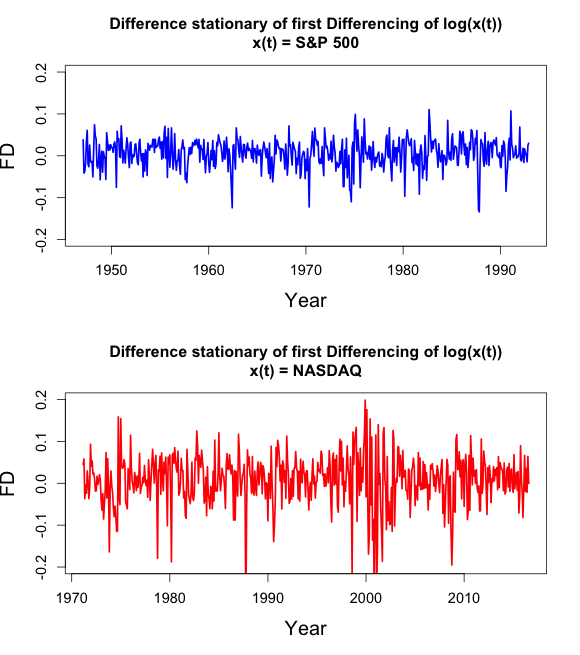
\includegraphics[scale=.65]{Images/DS}
\caption{Difference stationary of natural log a) SP500 b) NASDAQ.The difference stationary [ sp500(t2)-sp500(t1) and nasdaq(t2)-nasdaq(t1) ] provides insights on the variation of signal. The R program fdplot.R used to generate the graph is given in Appendix A}
\label{fig:DS}
\end{figure}

\textbf{Stationary Test:} There are several tests of stationary available and we used Dickey Fuller test (DF test) to test stationary of the first difference for logarithm of both indices. The $p-$value of DF test for logarithm of both indices is $0.001$ suggests that logarithm of both indices are difference stationary.  


\textbf{Deterministic Trend:} $\alpha \neq 0, \beta_1 \neq 0$, and $\beta_2=0$. $Y_t = \alpha + \beta_1 t + \mu_t$. Note that the mean of the series, $E(Y_t) = E(\alpha + \beta_{1}t) = \alpha + \beta_{1}t$, which is time-varying but its variance, \textit {$Var(\Delta Y_t) = Var(\alpha + \beta_{1}+u_t) = \sigma^2$} which is time-invariant. Still, the series with a deterministic trend is non-stationary. Once we know the values of $\alpha$ and $\beta_{1}$, we can subtract the mean from the series (detrending) and create a detrended series which is stationary. 


\textbf{Random walk with drift and deterministic trend:} $\alpha \neq 0, \beta_1 \neq 0$, and $\beta_2=1$. We get $Y_t = \alpha + \beta_{1}t + Y_{t-1} + u_t$. Note that the difference series, $\Delta Y_t = \alpha+\beta_{1}t+u_t$ is still time varying and hence, the mean of the differenced series is nonstationary. Detrending is still necessary on the differenced series to make it stationary. 


\subsection{Seasonal Trend Decomposition Procedure based on LOESS (STL)}
STL is a filtering procedure for decomposing a time series into trend, seasonal, and remainder components. STL has a simple design that consists of a sequence of applications of the LOESS (LOcal regrESSion) smoother; the simplicity allows analysis of the properties of the procedure and allows fast computation, even for a long time series and large amount of trend and seasonal smoothing. Other features of STL are specification of amounts of seasonal and trend smoothing that range, in a nearly continuous way, from a very small amount of smoothing to a very large amount; robust estimates of the trend and seasonal components that are not distorted by divergent behavior in the data. 

\begin{figure}[!ht]
\centering
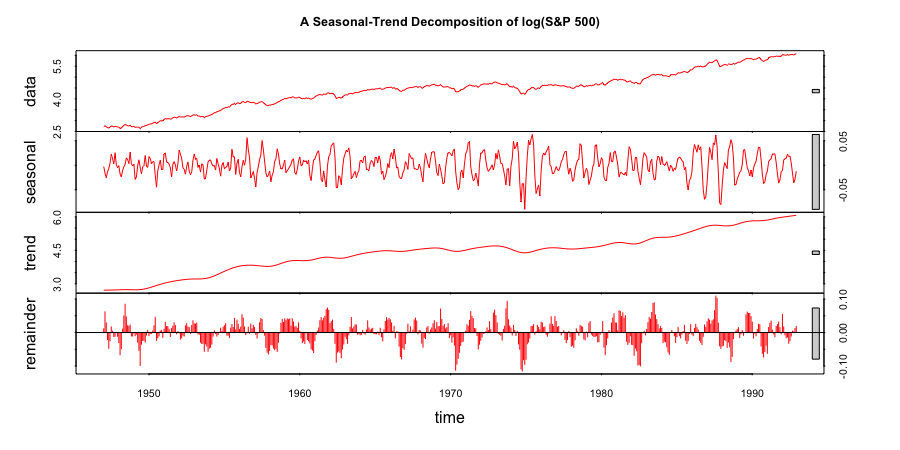
\includegraphics[scale=.5]{Images/STLSP500}
\caption{STL of Log SP500. a) The natural log of the SP500 b) The cyclical (or called seasonal) pattern c) The business trend of log SP500 d) Noise (remainder) data. The graph was created using the R program named as llt.R and it is attached in the Appendix A.}
\label{fig:STLSP500}
\end{figure}

A STL writes as $Y_t$, 

\begin{equation}
Y_t = f(S_t,T_t,E_t)
\end{equation} where $Y_t$ is time series data at time $t$, $S_t$ is seasonal component at time $t$, $T_t$ is trend component at time $t$ and $E_t$ is remainder (or error or irregular) component of data at time $t$ and $f$ is some function. For an additive decomposition $Y_t$ split up by
\begin{equation}
Y_t = S_t+T_t+E_t
\end{equation}

The user controls the variations on the trend and seasonal components.

In figure \ref{fig:STLSP500}, trend, seasonal and noise or error remainder data of the log of SP500 are extracted using the seasonal trend decomposition procedure. The seasonal window, in this case the value used is 5, is used to control the variation of the seasonal component. 


\begin{figure}[!ht]
\centering
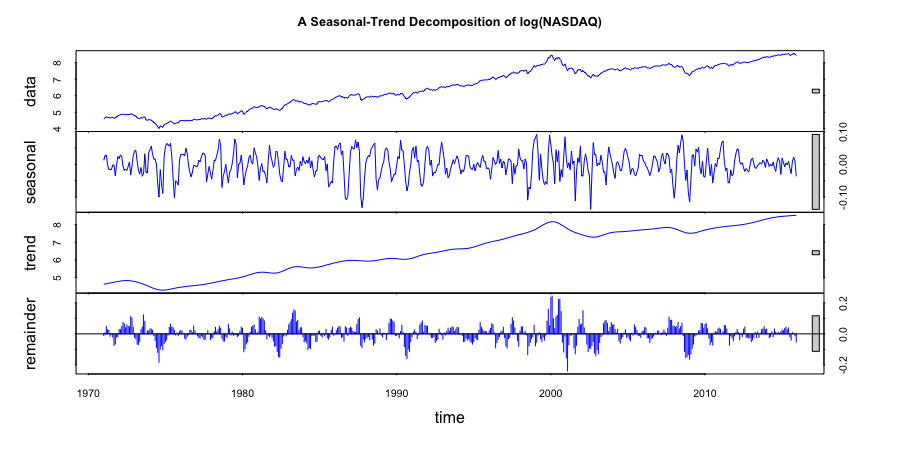
\includegraphics[scale=.5]{Images/STLNASDAQ}
\caption{STL of NASDAQ. a) The natural log of the NASDAQ b) The cyclical (or called seasonal) pattern c) The business trend of log NASDAQ d) Noise (remainder) data. The graph was created using the R program named as llt.R and it is attached in the Appendix A}
\label{fig:STLNASDAQ}
\end{figure}

In the figure \ref{fig:STLNASDAQ}, trend, seasonal and noise or error remainder data of the log of NASDAQ are extracted using the seasonal trend decomposition procedure. The seasonal window $(value = 5)$ is used to control the variation of the seasonal component. 

\subsection{Log-Linear Method}

When natural log values are used for the dependent variable and the independent variable is kept in its original scale, those models are called log linear models. 

The following model is of the value in a savings fund that depends on initial investment, growth rate and time duration in which the funds are invested. 

\begin{equation}
Y_t = Y_0{(1+r)}^t
\end{equation}
where $Y_t$ represents the value of the fund at the time $t$, $Y_0$ is the initial investment in the saving fund, and r is the growth rate.

\begin{figure}[!ht]
\centering
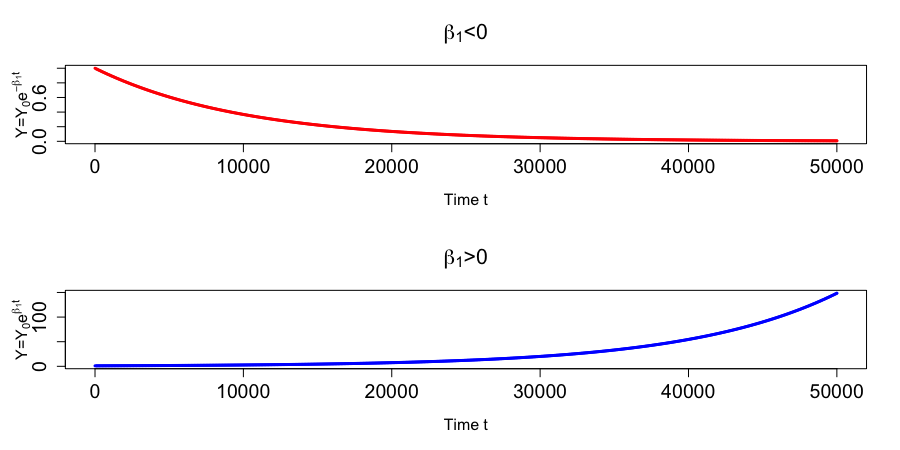
\includegraphics[scale=.5]{Images/LogLinear}
\caption{Log Linear Model when $\beta_1 < 0$ and when $\beta_1 > 0$. The graph was generated using loglinear.R, and it is attached in the Appendices A}
\label{fig:LogLinear}
\end{figure}
Taking log on both side, we obtain the following. 
\begin{equation}
log Y_t = log Y_0 + t log (1+r)
\end{equation}
Here $log Y_0$ is a constant and is taken to be $\beta_0$. Then $log (1+r)$ is taken to be $\beta_1$ and $log Y_t$ is given below:

\begin{equation}
log Y_t = {\beta}_0 + {\beta}_1 t
\end{equation}

\begin{figure}[!ht]
\centering
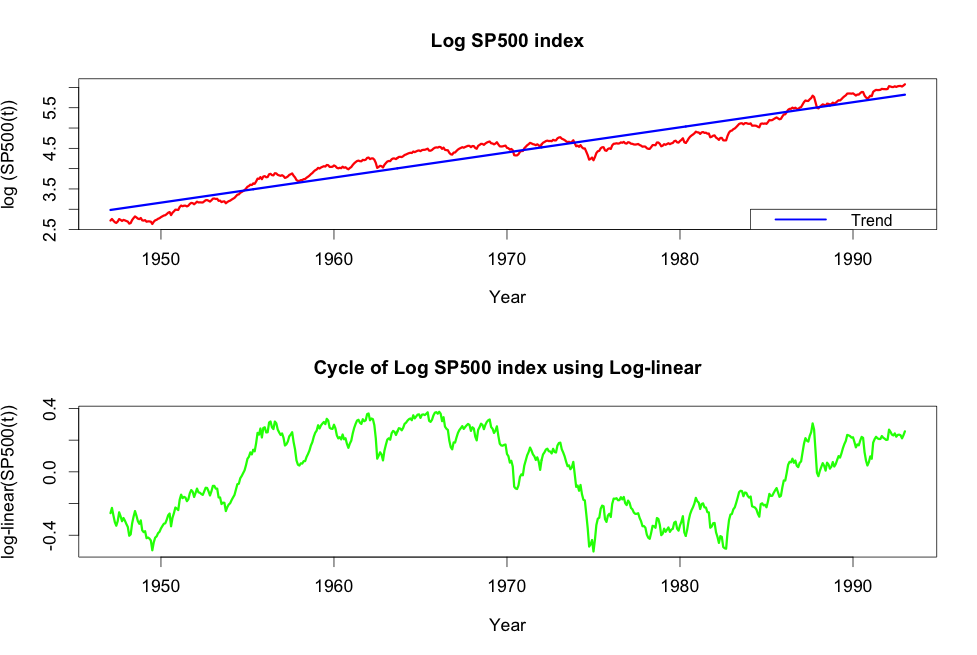
\includegraphics[scale=.5]{Images/lltcsp500}
\caption{Log linear of trend and cycle for log SP500 a) Log SP500 and trend. The trend is calculated based on estimation of slope and y-intersect  b)It is cycle of log-linear of SP500 and it is the variance of original log(sp500) and estimated trend. AutoCorrelation.R is the R program used to created the graph and it is attached in the Appendix A}
\label{fig:ACSP500}
\end{figure}

\begin{figure}[!ht]
\centering
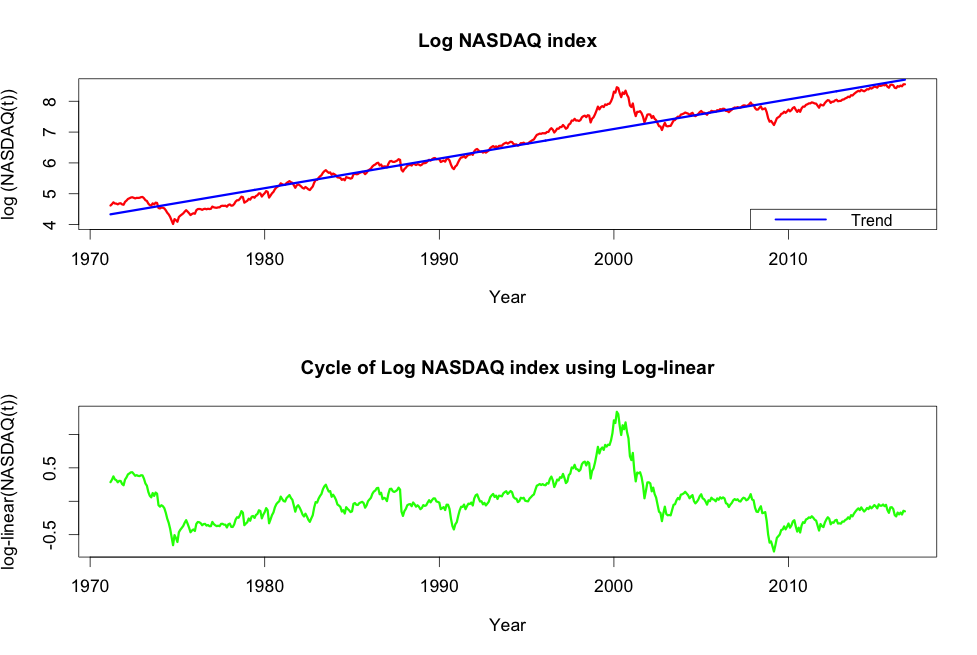
\includegraphics[scale=.5]{Images/lltcnasdaq}
\caption{Log linear of trend and cycle for log NASDAQ a) Log NASDAQ and trend. The trend is calculated based on estimation of slope and y-intersect  b)It is cycle of log-linear of SP500 and it is the difference between the original log(NASDAQ) and estimated trend. AutoCorrelation.R is the R program used to created the graph and it is attached in the Appendix A}
\label{fig:ACNASDAQ}
\end{figure}


After estimation of the log-linear model, the coefficients can be used to determine the impact of the independent variable $(t)$ on the dependent variable $(Y)$. The coefficient ${\beta}_1$ in a log-linear model represents the estimated percent change in the dependent variable for a unit change in independent variable. The coefficient ${\beta}_1$ provides the instantaneous rate of growth. The regression coefficients in the log-linear model do not represent the slope. 

When ${\beta}_1 > 0$, the log-linear function illustrates a positive impact from the independent variable and when, ${\beta}_1 < 0$, the log-linear function depicts a negative impact from the independent variable. 

\subsection{Auto correlation Functions}
An autoregressive model is when a value from a time series is regressed on previous value from that same time series. For exampe, $y_t$ on $y_{t-1}$:

\begin{equation}
y_t = \beta_{0} +\beta_{1}y_{t-1} +\epsilon_t
\end{equation}

In this regression model, the response variable in the previous time period has become the predictor and the errors have the same assumptions about errors in a simple linear regression model. The order of an autoregression is the number of immediate preceding values in the series that are used to predict the value at the present time. So, the preceding model is a first-order autoregression, written as $AR(1)$.

\begin{figure}[!ht]
\centering
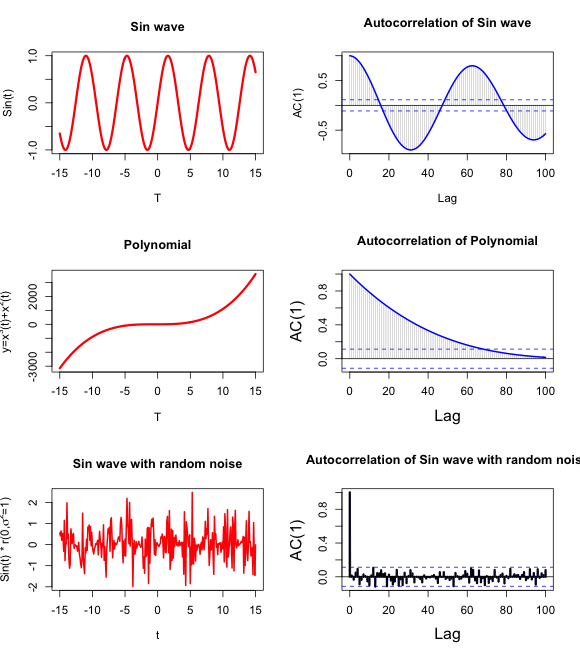
\includegraphics[scale=.65]{Images/ACExample}
\caption{Auto correlation for a) Sin wave b) Polynomial equation c) Sin wave with random noise. AutoCorrelation.R is the R program used to created the graph and it is attached in the Appendix A}
\label{fig:ACExample}
\end{figure}
\begin{figure}[!ht]
\centering
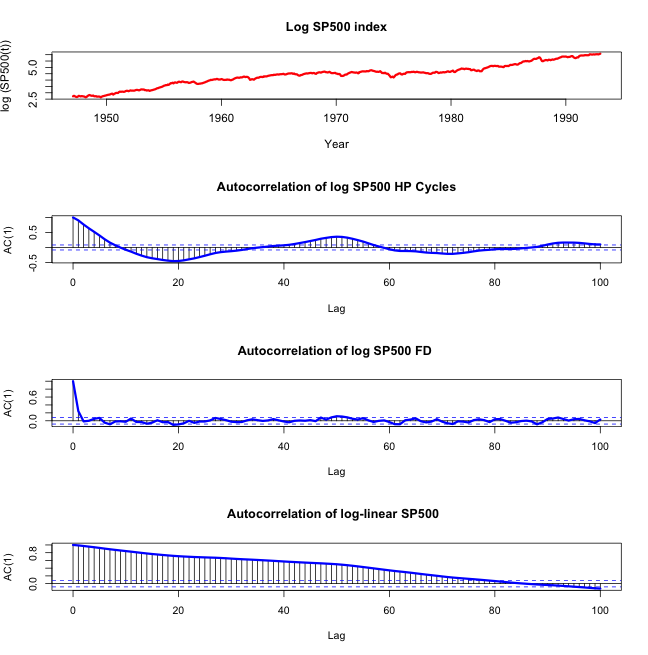
\includegraphics[scale=.65]{Images/ACSP500}
\caption{Auto correlation for log SP500 a) Log SP500 b)AutoCorrelation of HP cycle  c) Autocorrelation of First Differencing d) Autocorrelation of log-linear cycles of SP500. AutoCorrelation.R is the R program used to created the graph and it is attached in the Appendix A}
\label{fig:ACSP500}
\end{figure}
Let us say, if we want to predict the temperature $y$ this year $(y_t)$ using measurement of global temperature in the previous two years $(y_{t-1},y_{t-2})$. Then the autoregressive model for doing so would be:
\begin{equation}
y_t = \beta_{0} +\beta_{1}y_{t-1} +\beta_{2}y_{t-2}+\epsilon_t
\end{equation}

The above model is a second-order autoregression, written as $AR(2)$, since the value at time $t$ is predicted from the values at times $t-1$ and $t-2$. More generally, $k^{th}$ order autoregression, written as $AR(k)$, is a multiple linear regression in which the value of the series at any time $t$ is a linear function of the values at times $t-1,t-2,...,t-k$.

\begin{figure}[!ht]
\centering
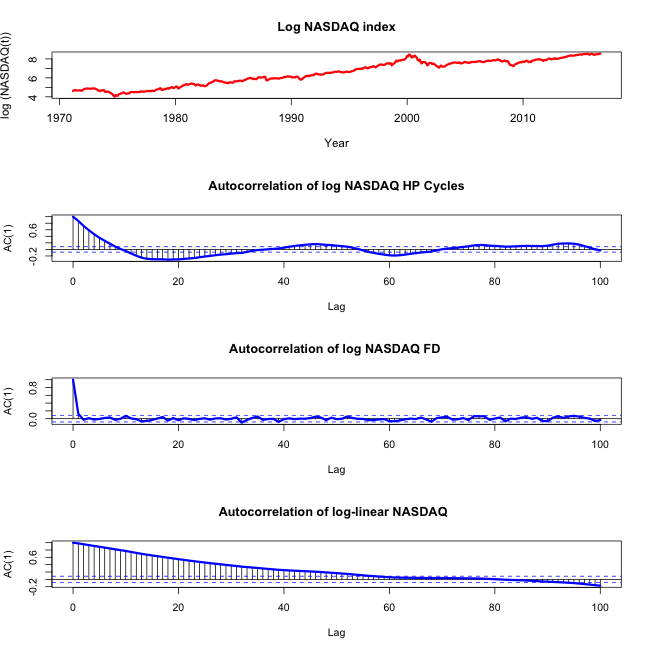
\includegraphics[scale=.65]{Images/ACNASDAQ}
\caption{Auto correlation for log NASDAQ a) Log NASDAQ b)AutoCorrelation of HP cycle  c) Autocorrelation of First Differencing d) Autocorrelation of log-linear cycles of NASDAQ. AutoCorrelation.R is the R program used to created the graph and it is attached in the Appendix A}
\label{fig:ACNASDAQ}
\end{figure}
The cofficient of correlation between two values in a time series is called the \textbf{autocorrection function} $(ACF)$. Let $y_t$ be a sample, $t = 1,2,..,n$ from an ARMA process of possibly unknown order, then the $j^{th}$ order auto correlation $\rho(j)$ can be esimated by using the formula
\begin{equation}
\rho(j) = \frac{Cov(y_t,y_{t-j})}{Var(y_t)}
\end{equation}
where
\begin{equation}
Cov(y_t,y_{t-j}) = \frac{1}{n-1} \sum_{t=j+1}^{n}(y_t-y_\mu)(y_{t-j}-y_\mu)
\end{equation}
\begin{equation}
Var(y_t)= \frac{1}{n-1} \sum_{t=1}^{n}(y_t-y_\mu)^2
\end{equation}
$y_\mu$ is the mean of the $y_t$.
\subsection{Hodrick and Prescott (HP) filter}
Hodrick and Prescott proposed the HP filter to decompose a macroeconomic time series into a non-stationary trend component and a stationary cyclical residual component. The filter has become popular in applied macro economics in the last 15 years.  Given an observed series $y_i$, let $y_i = x_i + c_i$, with $y^T = (y_1,y_2..., y_N), x^T = (x_1,x_2,....x_N)$ and $c^T = (c_1,c_2...., c_N)$ where $x_t$ denotes the unobserved trend component at time $t$ and $c_t$ the unobserved cyclical residual at time $t$. The HP trend $\hat{x}$ can be obtained as the solution to the following convex minimization problems:



\begin{equation}
\min_{[x_t]_{t=1}^{N}}  \begin{bmatrix} \sum_{t=1}^{N} (y_t - x_t)^2 +\lambda \sum_{t=2}^{N-1} ( ( x_{t+1} - x_t) - (x_t - x_{t-1}))^2  \end{bmatrix}
\end{equation}

Here, $\lambda$ is usually known as the smoothing parameter. As $\lambda$ becomes larger, the HP estimated trend curve becomes smoother. The term being squared in the second sum of the equation, $( x_{t+1} - x_t) - (x_t - x_{t-1})$, or $\bigtriangleup^{2}x_i$, is an approximation to the second derivate of $x$ at time $t$. There are two opposing forces in the HP minimization problem. One force is attempting to minimize the sum of squared cyclical residuals and the other force is attempting to minimize the sum of squared $\bigtriangleup^{2}x_i$. The smoothing parameter, $\lambda$, gives relative weight to these two opposing forces. 

\begin{table}[h!]
\centering
\begin{tabular}{||c c c c c c ||} 
 \hline
 Detrending & Mean & SD & Variance & $T_{0}$ (month) & $P_{dc}$ (year) \\ [0.5ex] 
 \hline\hline
 FD & 0.011 & 0.1123 & 0.0126 & 1.94 & 00.7 \\
 HP & 0.008 & 0.2686 & 0.0722 & 8.93 & 02.9 \\
 LLD & 0.426 & 0.3265 & 0.1066 & 85.6 & 28.5  \\
 \hline
\end{tabular}
\caption{Detrend Statistics on S\&P 500. The value for the above table was created by using the Matlab program DetrendStatistics.m attached in the appendix.  }
\label{table:sp500trendstat}
\end{table}


\begin{table}[h!]
\centering
\begin{tabular}{||c c c c c c ||} 
 \hline
 Detrending & Mean & SD & Variance & $T_{0}$ (month) & $P_{dc}$ (year) \\ [0.5ex] 
 \hline\hline
 FD & 0.008 & 0.1072 & 0.0115 & 1.81 & 00.6 \\
 HP & 0.022 & 0.2256 & 0.0509 & 9.22 & 03.0 \\
 LLD & 0.258 & 0.3159 & 0.0992 & 80.5 & 26.8  \\
 \hline
\end{tabular}
\caption{Detrend Statistics on NASDAQ. The value for the above table was created by using the Matlab program DetrendStatistics.m attached in the appendix.  }
\label{table:sp500trendstat}
\end{table}

The $\lambda$ parameter determines the smoothness of the trend component. The larger the value of $\lambda$, the higher the penalty in the  second term.  An empirical study indicates that a $5\%$ cyclical component is moderately large, as is a $1/8$th of $1\%$ change in the growth rate in a quarter. In the paper \cite{lambdaforhp}, $\lambda$ should be adjusted by multiplying it with the fourth power of the observation frequency ratios. This yields an HP parameter value of 6.25 for annual data given a value of 1600 for quarterly data. 

\subsubsection{First-order conditions of the HP minimization problem}

The following HP first order conditions are derived by setting the gradient vector of the above minimization equation equal to zero. The first-order conditions are:
\begin{flushleft}
\begin{align}
c_1&=\lambda(x_1-2x_2+x_3)  \nonumber \\
c_2&=\lambda(-2x_1+5x_2-4x_3+x_4) \nonumber \\
c_t&=\lambda(x_{t-2}-4x_{t-1}+6x_t-4x_{t+1}+x_{t+2}), t=3,4,5,....,N-2 \nonumber \\
c_{N-1}&=\lambda(x_{N-3}-4x_{N-2}+5x_{N-1}-2x_N) \nonumber \\
c_{N}&=\lambda(x_{N-2}-2x_{N-1}+x_N) \nonumber
\end{align}
\end{flushleft}
or more compactly, 
\begin{center}
\boldmath{$c=\lambda Fx$}
\end{center}
\unboldmath
where F = 
\begin{flushright}
$\begin{bmatrix}
1 & -2 & 1 & 0 & \cdots & \cdots & \cdots &\cdots & & 0 \\
-2 & 5 & -4 & 1 & 0 & \cdots & \cdots & & & 0 \\
1 & -4 & 6 & -4 & 1 & 0 & \cdots &  & & 0 \\
0 & 1 & -4 & 6 & -4 & 1 & 0 & \cdots & &  0 \\
0 & 0 & 1 & -4 & 6 & -4 & 1 & 0  &\cdots  & 0 \\
\vdots & & & & & & & & & \vdots \\
\vdots & & & & & & & & & \vdots \\
\vdots & & & & & & & & & \vdots \\
0 & \cdots & \cdots & 0 & 1 & -4 & 6 & -4 & 1 & 0 \\
0 & \cdots & & \cdots &   0 & 1 & -4 & 6 & -4 & 1 \\
0 & \cdots & \cdots &  &  & 0 & 1 & -4 & 5 & -2 \\
0 & \cdots & \cdots & \cdots &  &  & 0& 1 & -2 & 1 
\end{bmatrix}$
\end{flushright}

which implies that 

\begin{center}
\boldmath{$y=(\lambda F+I)x$}
\unboldmath
\end{center}
Thus, the HP trend is given by:
\begin{center}
\boldmath{$\hat{x}=(\lambda F+I)^{-1}y$}
\unboldmath
\end{center}
and
\begin{center}
\boldmath{$\hat{c}=y-\hat{x}$}
\unboldmath
\end{center}

\begin{figure}[!ht]
\centering
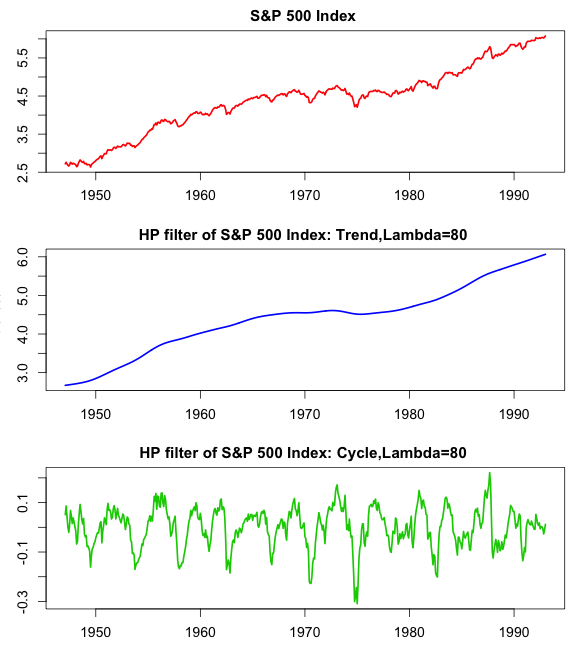
\includegraphics[scale=.65]{Images/SP500HP80}
\caption{The trend and cycle separation from SP500 using HP filter with $\lambda$ = 80. a) Natural Log of SP500 index b) Trend extracted from Log of SP500 index using HP filter c) Cyclical pattern extracted from SP500 index using HP filter}
\label{fig:SP500HP80}
\end{figure}

In the figure \ref{fig:SP500HP80}, the $\lambda$ value is 80 and the trend and cyclical information is separated from the natural log SP500 index and the trend data is useful for the long term investors like pension fund manager. The long term fund managers require the projection of the performance of an index to strategize the investment to meet the client's retirement objective. 

\begin{figure}[!ht]
\centering
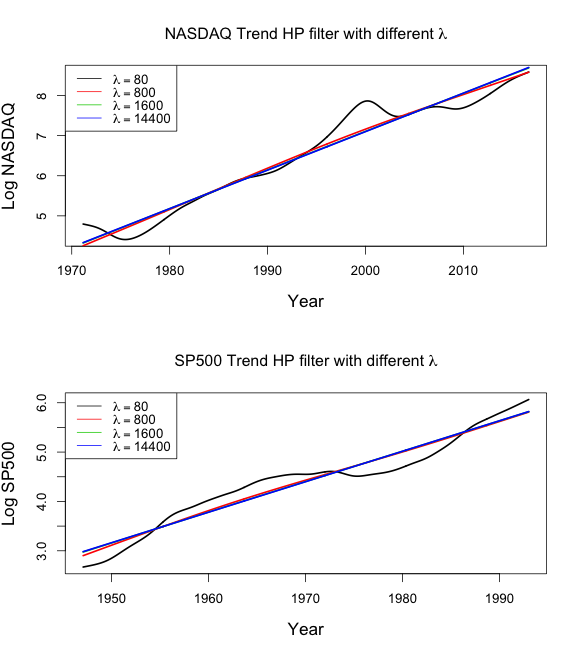
\includegraphics[scale=.65]{Images/Lambda}
\caption{HP filter with different value for $\lambda$ a) NASDAQ b) S\&P 500}
\label{fig:Lambda}
\end{figure}
In the figure \ref{fig:Lambda}, the SP500 trend analysis was performed using different $\lambda$ values. The trend looks very similar when the $\lambda$ is above 800 value and there is no significance when the $\lambda$ values are at 1600, 14400. The above figure \ref{fig:Lambda}, indicates that when $\lambda$ is above 800 or above the trend in the HP filter is very close to least square linear regression line. 

\begin{figure}[!ht]
\centering
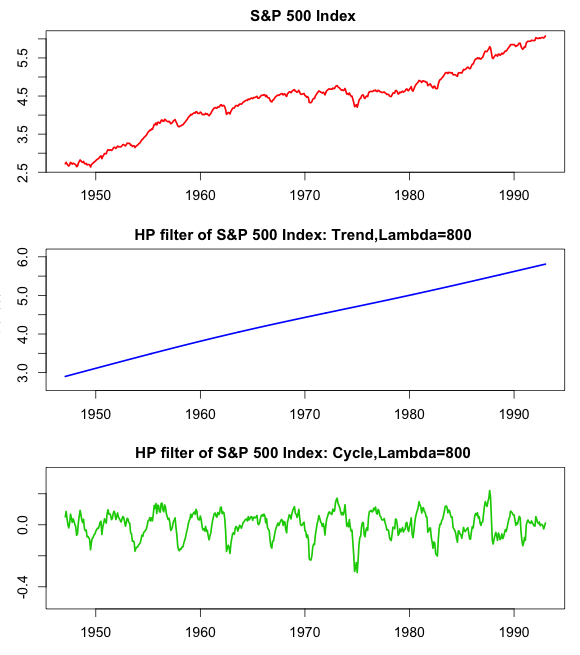
\includegraphics[scale=.65]{Images/SP500HP800}
\caption{The trend and cycle separation from SP500 using HP filter with $\lambda$ = 800. a) Natural Log of SP500 index b) Trend extracted from Log of SP500 index using HP filter c) Cyclical pattern extracted from SP500 index using HP filter }
\label{fig:SP500HP800}
\end{figure}
In the figure \ref{fig:SP500HP800}, the $\lambda$ value is 800  and a similar analysis was performed.


\begin{figure}[!ht]
\centering
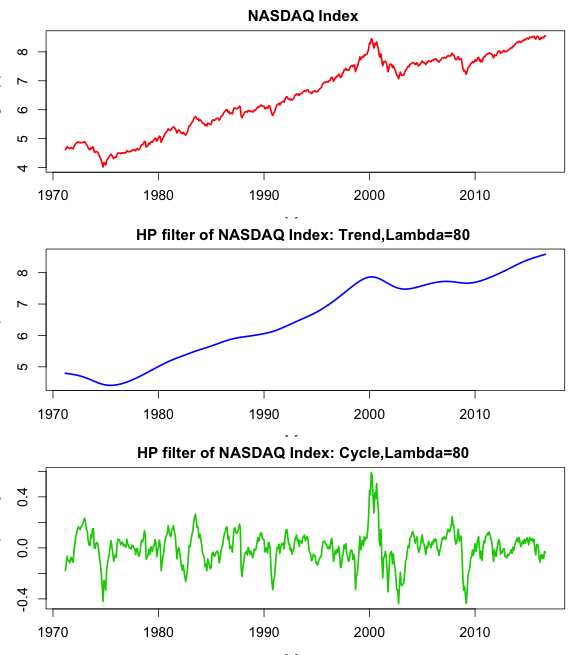
\includegraphics[scale=.65]{Images/NASDAQHP80}
\centering
\caption{The trend and cycle separation from NASDAQ using HP filter with $\lambda$ = 80. a) Natural Log of NASDAQ index b) Trend extracted from Log of NASDAQ index using HP filter c) Cyclical pattern extracted from NASDAQ index using HP filter }
\label{fig:NASDAQHP80}
\end{figure}
In the figure \ref{fig:NASDAQHP80}, the $\lambda$ value is 80 and the trend and cyclical information is separated from the natural log NASDAQ index.


In the figure \ref{fig:Lambda}, the NASDAQ trend analysis was performed using different $\lambda$ values. The trend looks very similar when the $\lambda$ is above 800 value and there is no signficance when the $\lambda$ values are at 1600, 14400.
\begin{figure}[!ht]
\centering
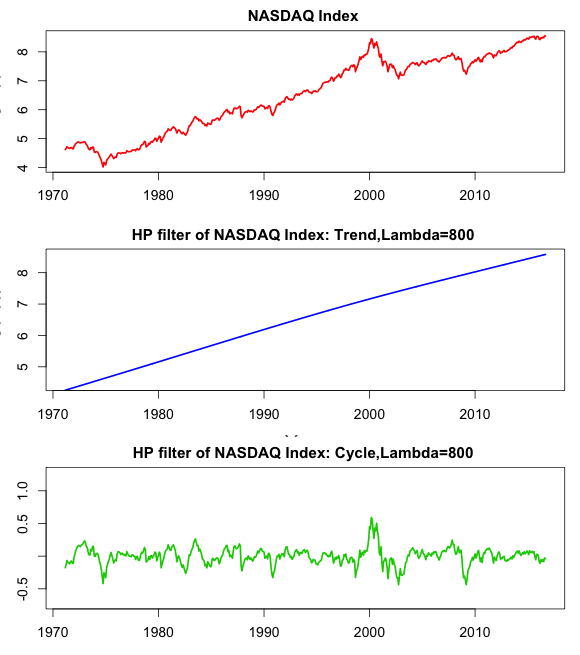
\includegraphics[scale=.65]{Images/NASDAQHP800}
\caption{The trend and cycle separation from NASDAQ using HP filter with $\lambda$ = 800. a) Natural Log of NASDAQ index b) Trend extracted from Log of NASDAQ index using HP filter c) Cyclical pattern extracted from NASDAQ index using HP filter }
\label{fig:NASDAQHP800}
\end{figure}

The HP filters is one of the most heavily used econometric methods for measuring business cycles and potential output in empirical research. It is also a smoothing method that belongs to a very general class of nonparametric graduation procedures that depend on a tuning parameter governing the properties of the smoother. The long run potential output of an economy can be substantially influenced by great recessions and depressions, which may sufficiently divert resources to impact long run trend components of output. The HP filter has the advantage that, depending on the smoothing parameter $(\lambda)$ choice, it can encompass long run behavior that encompasses a vast range of possibilities -from a deterministic linear trend, to a smooth Gaussian process, through to stochastic trends and combination of stochastic trends and deterministic trends that even include trend breaks. 

. 


\chapter{Introduction}
\label{chap:Intro}
\input{Intro/Intro}


\chapter{Gabor Transformation}
\label{chap:Gabor}
\section{Signal Processing}
An arbitrary signal given by a function $f(t)$ can be represented by many forms for better understanding of the signal. The representation of the signal $f(t)$ in a different form depends on the type of application the user is interested in. In few cases, the original signals are perfectly fine as is for a given application.

In signal processing there are two major fields of study.
\begin{itemize}
  \item  {Signal synthesis - Construction of a signal}
  \item  {Signal analysis - Study of a signal}
\end{itemize}

Gabor in his original paper - Theory of communication \cite{gabor}, stated that a time function $f(t)$ in the time interval $\tau$ = \{${s:t_1<s<t_2}$\}  contains an infinite amount of data. There are an infinite number of ways to represent $f(t)$ in the interval $\tau$ and one of the ways is to represent $f(t)$ in the interval $\tau$ by a polynomial of order $N$. For example, one can fit $f(t$) as closely as possible by the method of least squares and take the coefficients of the polynomial as data. The polynomial coefficients of the curve is the data that represents the curve in the interval.  It is equivalent to specifying the polynomial in such a way that its first $N+1$ moments $M_i$ shall be equal to those of $f(t)$. 
\begin{equation*}
\begin{aligned}
M_0 =& \int_{t_1}^{t_2}{f(t)dt}; \\
M_1 =& \int_{t_1}^{t_2}{tf(t)dt}; \\
M_2 =& \int_{t_1}^{t_2}{t^2f(t)dt};\\
.. \\
M_{N-1} =& \int_{t_1}^{t_2}t^{N-1}{f(t)dt} \\
M_{N} =& \int_{t_1}^{t_2}t^{N}{f(t)dt}
\end{aligned}
\end{equation*}
Instead of the polynomial coefficients, the moments are considered as the specific data. If the purpose is to transmit the signal, then the moments (equivalent of polynomial coefficients) can be transmitted and the signal can be reconstructed at the other end.
Instead of representing the function $f(t)$ in the interval $\tau$ in terms of powers of time functions, it can be represented in terms of orthogonal functions ${\phi}_k(t)$ in the interval $\tau$. How close the fit will be depends on the set of orthogonal functions selected and type of applications.
\subsection{Sampling Theorem}
The Sampling theorem states that for an accurate representation of a signal $f(t)$ by its time samples $f(nT)$, two conditions must be met. 
\begin{itemize}
  \item  {The signal $f(t)$ must be band limited, that is, its frequency spectrum must be limited to contain frequencies up to some maximum frequency, say $S_{max}$, and no frequencies beyond that.}
  \item  {The sampling rate $S_s$ must be chosen to be at least twice the maximum frequency $S_{max}$, that is, $S_s \ge 2 S_{max}$ or, in terms of the sampling time interval: $T \le \frac{1}{2S_{max}}$.}
\end{itemize}

The minimum sampling rate allowed by the sampling theorem, that is, $S_s = 2S_{max}$, is called the $\textbf Nyquist$ rate. For arbitrary values of $S_s$, the quantity $\frac{S_s}{2}$ is called the $\textbf Nyquist$ frequency. It defines the endpoints of the Nyquist frequency interval [$-\frac{S_s}{2},\frac{S_s}{2}$]. 

\subsection{Rayleigh Frequency}
The lowest resolvable frequency interval is given by the inverse of the length of the analysis window and is denoted by the $\textbf Rayleigh$ frequency, $S_r = \frac{1}{L}$. The frequency resolution of any signal to be analyzed depends on the Rayleigh frequency of the data. 

\section{Fourier Transformation}
If the orthogonal function set is simple harmonic functions sine and cosine in the interval extending from ${-\infty}$ to ${\infty}$, then the given signal is presented in the frequency domain and it is called the Fourier transformation.


\begin{equation}
F(s) = \int_{-\infty}^{\infty}{f(t)e^{-j2\pi ts}dt}
\end{equation}
$F(s)$ is the Fourier transform of $f(t)$. The inverse Fourier transform function $F(s)$ provides the function $f(t)$ and the equation for this is given below.
\begin{equation}
f(t) = \int_{-\infty}^{\infty}{F(s)e^{j2\pi ts}ds}
\end{equation}

Fourier transformation is a tool to translate a signal from time domain to frequency domain and vice versa. In fact, it is an apt tool to analyze a signal in the frequency domain given the signal does not evolve over time, but, most of the practical signals like music, seismic and others evolve over time. It is challenging to study and understand the insights of those signals in the frequency domain by just using Fourier transformation. In recent years, there are many ideas proposed to overcome that challenge and gain more insights of the signals in other domains. 

\begin{figure}[!ht]
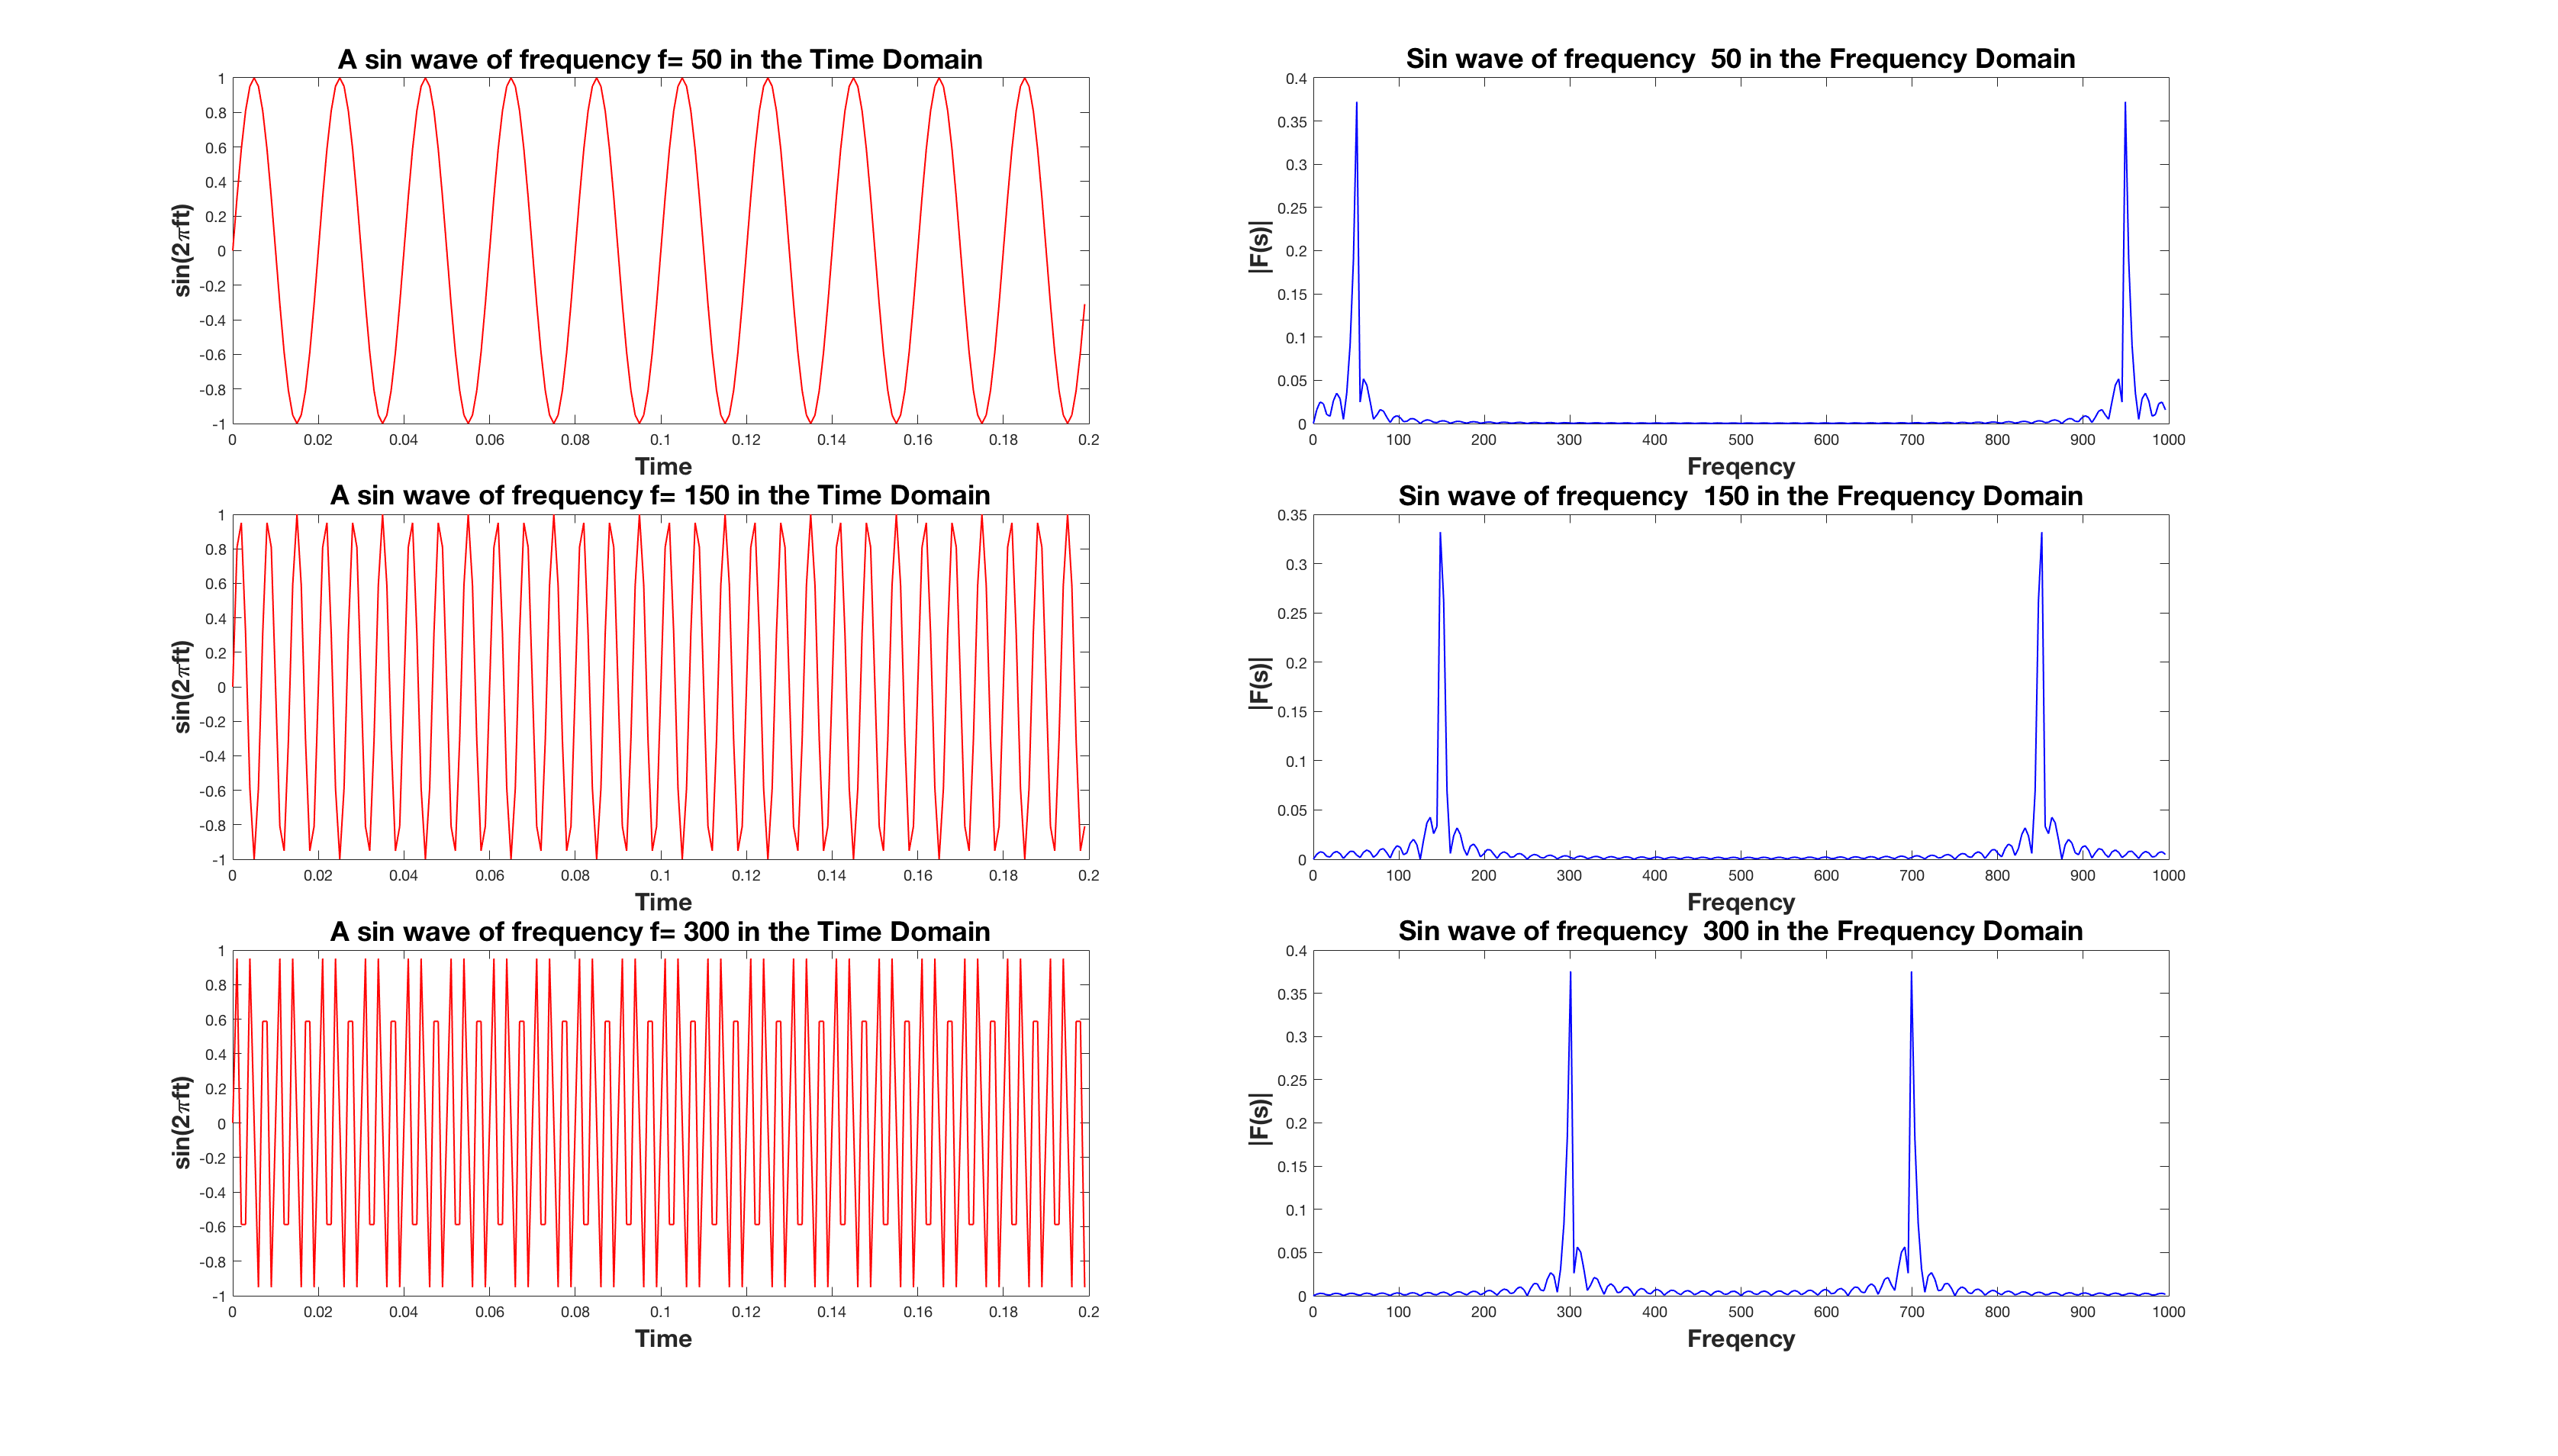
\includegraphics[scale=.15]{Images/fourier-sin}
\caption{Fourier Transforms for discretized time signal sine waves with three different frequencies and respective discrete Fourier transforms are given above. The sampling period used is 0.001 and total length of signal (L) is 200. The graphs were created using Matlab code DrawSinFourierGraph.m and it is attached in the Appendix B}
\label{fig:Fourier-sin}
\end{figure}

In the figure \ref{fig:Fourier-sin}, a sine wave with different frequencies ${f = 50,150,300}$ is transformed into the frequency domain using the discrete Fourier transform. Please note high amplitude in the frequency domain for their respective frequency in each graph. $\omega = 2\pi f$.

\begin{equation}
f(t) = \sin(\omega t) 
\end{equation}
Three types of sine wave are created with frequencies ${f =50, 150,300}$. The Fourier transform of the $f(t)$ is given by
\begin{equation}
\begin{split}
F(s)  &= \int_{-\infty}^{\infty}{\sin(2\pi f t) e^{-j2\pi t s }dt} \\
 \int_{-\infty}^{\infty}{\sin(2\pi f t) e^{-j2\pi t s }dt}  &= \frac{\delta(t-2\pi f) - \delta(t+2\pi f)}{2j}
 \end{split}
\end{equation}
Where $\delta(s)$ is the Dirac Delta function. The Dirac Delta function is defined as
$$
\delta(t) = \left\{ \begin{array}{rl}
 +\infty  &\mbox{ if $t=0$} \\
   0 &\mbox{ if $t\ne0$}
          \end{array} \right.
		  $$
\begin{equation}
\int_{-\infty}^{\infty} \delta(t) dt = 1 
\end{equation}
It follows that
\begin{equation}
\int_{-\infty}^{\infty} a \delta(t) dt = a 
\end{equation}
where a is a constant. 

For a function $f(t)$, being integrable, we have that
\begin{equation}
\int_{-\infty}^{\infty}  f(t) \delta(t) dt = f(0)
\end{equation}
It denotes that the integral of any function multiplied by a $\delta$-function located about zero is just the value of the function at zero. This concept can be extended to give the shifting property, again for a function $f(t)$, giving, 
\begin{equation}
\int_{-\infty}^{\infty}  f(t) \delta(t-a) dt = f(a)
\end{equation}
where $\delta(t-a)$ is just a $\delta$-function located at $t = a$. 
In two dimensions, for a function $f(t,w)$, we have that,
\begin{equation}
\int\int  f(t,w) \delta(t-a,w-b) dt dw = f(a,b)
\end{equation}
where $\delta(t-a,w-b)$ is a $\delta$-function located at position $a,b$. This property is central to the idea of convolution, which is used extensively in image formation theory, and in digital image processing. 
The Fourier transform of a $\delta$ function can be formed by direct integration using the definition of the Fourier transform, and the shift property. We get, 

\begin{equation} \label{eq:delta1}
\begin{split}
F(\delta(t)) & = \int_{-\infty}^{\infty} \delta(t) e^{-j2\pi s t} dt \\
 & = e^0 \\
 & = 1
 \end{split}
\end{equation}

\subsection{Shifting Theorem}
Let $f(t)$ be a function and its Fourier transform is given by $F(s)$. Fourier transform of a function $f(t-t_0)$ is given $e^{-j2\pi s t_0}F(s)$. The proof of the shift theorem is given below. $F[f(t-t_0)](s) = e^{-j 2 \pi s t_0} F(s)$

\begin{equation} 
F[f(t-t_0)](s) = \int_{-\infty}^{\infty} f(t-t_0)  e^{-j2\pi s t} dt 
\end{equation}
Multiply $e^{j2\pi s t_0} e^{-j2\pi s t_0} $ on right hand side of the above equation.
\begin{equation} 
\begin{split}
F[f(t-t_0)](s) &= \int_{-\infty}^{\infty} f(t-t_0) e^{-j2\pi s t} e^{j2\pi s t_0}  e^{-j2\pi s t_0} dt \\
& = e^{-j2\pi s t_0}  \int_{-\infty}^{\infty} f(t-t_0) e^{-j2\pi s (t-t_0)} dt 
 \end{split}
\end{equation}
Let $u = t-t_0$
\begin{equation} 
\begin{split}
F[f(t-t_0)](s) &= \int_{-\infty}^{\infty} f(u) e^{-j2\pi s u} du \\
& = e^{-j2\pi s t_0}  F(s)
 \end{split}
\end{equation}

By applying the shifting theorem in the equation \ref{eq:delta1},we get that, 
\begin{equation}
F(\delta(t-a)) = e^{-j2\pi s a}
\end{equation}
so that the Fourier transform of a shifted $\delta$ function is given by a phase ramp. The modulus squared of above equation is
\begin{equation}
\begin{split}
|F(\delta(t-a))|^2 & = |e^{-j2\pi s a}|^2 \\
& = 1
\end{split}
\end{equation}
The power spectrum of a $\delta$ function is constant independent of its location in real space. Noting that the Fourier transform is a linear operator, consider two $\delta$ functions located at $\pm a$. Then the Fourier transform of $\delta(t-a)+\delta(t+a)$ is given by
\begin{equation}
\begin{split}
F(\delta(t-a)+\delta(t+a)) & = e^{-j2\pi as}+e^{j2\pi as}\\
& = 2\cos(2 \pi as) \\
\int_{-\infty}^{\infty} \cos(2 \pi a t) e^{-j2\pi t s} &= \frac{\delta(t-a)+\delta(t+a)}{2}
\end{split}
\end{equation}
If we take the $\delta$-function at $t=-a$ as negative, the Fourier transform is given below
\begin{equation}
\begin{split}
F(\delta(t-a)-\delta(t+a)) & = e^{-j2\pi as}-e^{j2\pi as}\\
& = 2j\sin(2 \pi as) \\
\int_{-\infty}^{\infty} \sin(2 \pi a t) e^{-j2\pi t s} &= \frac{\delta(t-a)-\delta(t+a)}{2j}
\end{split}
\end{equation}
\begin{figure}[!ht]
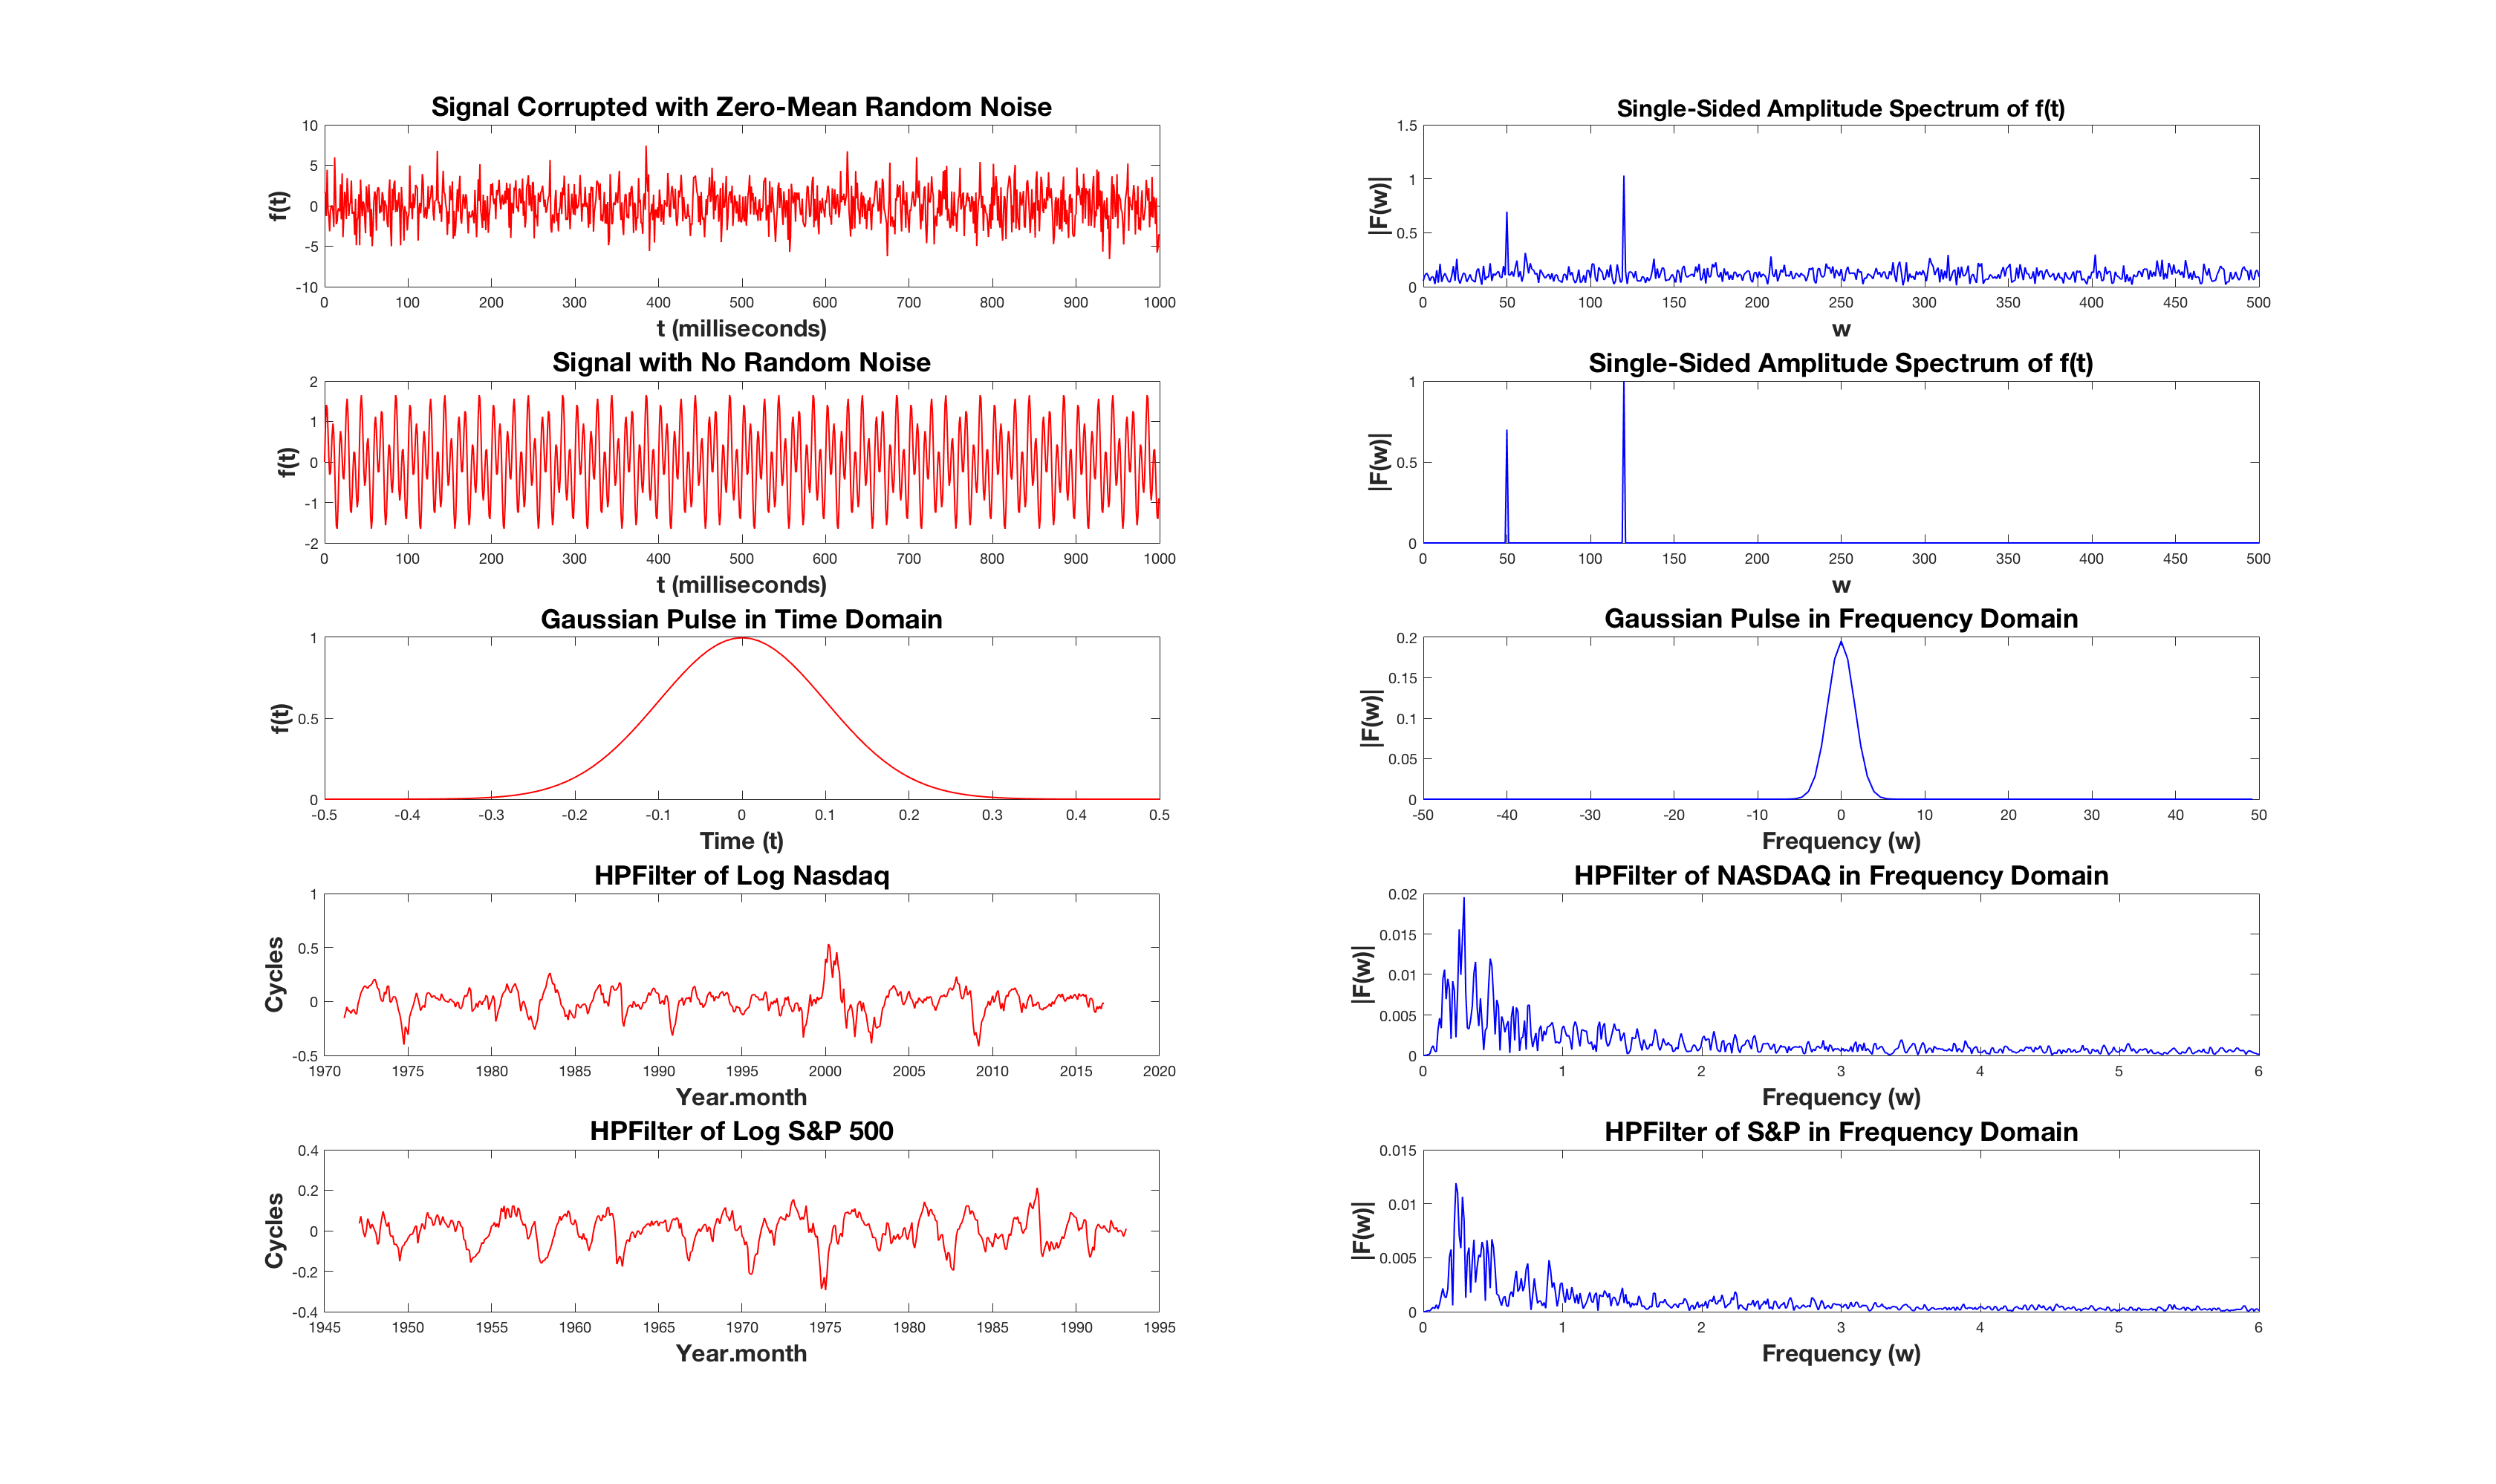
\includegraphics[scale=.15]{Images/fourier3}
\caption{Fourier transform for a) Zero mean signal with random noise, b) Zero mean signal $f(t) = 0.7sin(2\pi 50t)+sin(2\pi 120t)$, c) Gaussian - Frequency are shifted (using fftshift function in matlab) in the frequency domain to show that the Fourier transform of Gaussian looks like Gaussian in the frequency domain, d) HP Filter of Log NASDAQ, e) HP Filter of Log S\&P 500. The program used to generate the graph is SPNASDAQFourier.m and stored in Appendix }
\label{fig:Fourier3}
\end{figure}
In the figure \ref{fig:Fourier3}, a signal with zero mean random noise, signal with zero mean with no random noise, Gaussian curve, HP filter of $log$ sp500, HP filter of $log$ Nasdaq are also transformed into a  frequency domain using the discrete Fourier transform. $|F(s)|$ is an even function and so only $s>0$ is shown in figure \ref{fig:Fourier3}.
\subsection{Discrete Fourier Transform}
The Discrete Fourier Transform (DFT) is the equivalent of the continuous Fourier Transform for signals known only at N instants separated by sample times T (i.e a finite sequence of data). Let $f(k)$ be a continuous signal and the $N$ samples be denoted by $f(0), f(1), f(2)... f(k),...,f(N-1)$. Each sample $f(k)$ is regarded as an impulse having area $f(k)$ and the integrand exists only at the sample points.
\begin{comment}
\begin{align}
F(j2\pi s) &= \int_{0}^{(N-1)T}{f(t)e^{-j2\pi ts}dt}; \\
&= f[0]e^{-j0} + f(1)e^{-j2\pi sT}+...+f(k)e^{-j2\pi skT}+....f(N-1)e^{-j2\pi(N-1)T} \\
&= \sum_{k=0}^{N-1} f(k) e^{-j2\pi sk T}
\end{align}
\end{comment}
Since there are only a finite number of input data points, the DFT treats the data as if it were periodic i.e $f(N)$ to $f(2N-1)$ is the same as $f(0)$ to $f(N-1)$. In general, the discrete Fourier Transform is given by
\begin{equation}
F(s) = \sum_{k=0}^{N-1} f(k) e^{-j\frac{2\pi}{N} sk }
\end{equation}
$s = 0,1,..,N-1$.
\begin{equation}
e^{j\frac{2\pi}{N}} = \cos(\frac{2\pi}{N}) + j \sin(\frac{2\pi}{N})
\end{equation}
is the principal N-th root of unity. Since $ e^{j\frac{2\pi s}{N}}$ has a period of N, the DFT coefficients $F(s)$ are periodic with period N when $s$ is taken outside the range $s = 0,1,2,...N-1$. $F(s)$ is the Discrete Fourier Transform of the sequence $f(t)$. The matrix-vector format of the Discrete Fourier Transform are given by

$\underbrace{
\begin{bmatrix}
F(0) \\
F(1) \\
F(2) \\
\vdots \\
\vdots \\
F(N-1)
\end{bmatrix} }_{\text{DFT Vector} }$ \qquad
=
$\underbrace{
\begin{bmatrix}
1 & 1 & \cdots & \cdots & 1 \\
1 & e^{-j(\frac{2\pi}{N})} & e^{-j(\frac{4\pi}{N})}\cdots & \cdots & e^{-j\frac{2(N-1)\pi}{N}} \\
1 & e^{-j(\frac{4\pi}{N})} & e^{-j(\frac{8\pi}{N})}\cdots & \cdots &  e^{-j\frac{4(N-1)\pi}{N}} \\
\vdots & & & \vdots \\
\vdots & & & \vdots \\
1 & e^{-j(\frac{2(N-1)\pi}{N})} & e^{-j(\frac{4(N-1)\pi}{N})}\cdots & \cdots & e^{-j\frac{2(N-1)(N-1)\pi}{N}} \\
\end{bmatrix} }_{\text{DFT Matrix:F}}$
$\underbrace{
\begin{bmatrix}
f(0) \\ f(1) \\ f(2) \\ \vdots \\ \vdots \\ f(N-1) 
\end{bmatrix}}_{\text{Input Signal}}$

The above matrix multiplication can also be used to compute the Discrete Fourier Transform of a given signal $f(t)$.  The Discrete Fourier Transform matrix F can be precomputed as it is independent of the input signal. 

\begin{figure}[!ht]
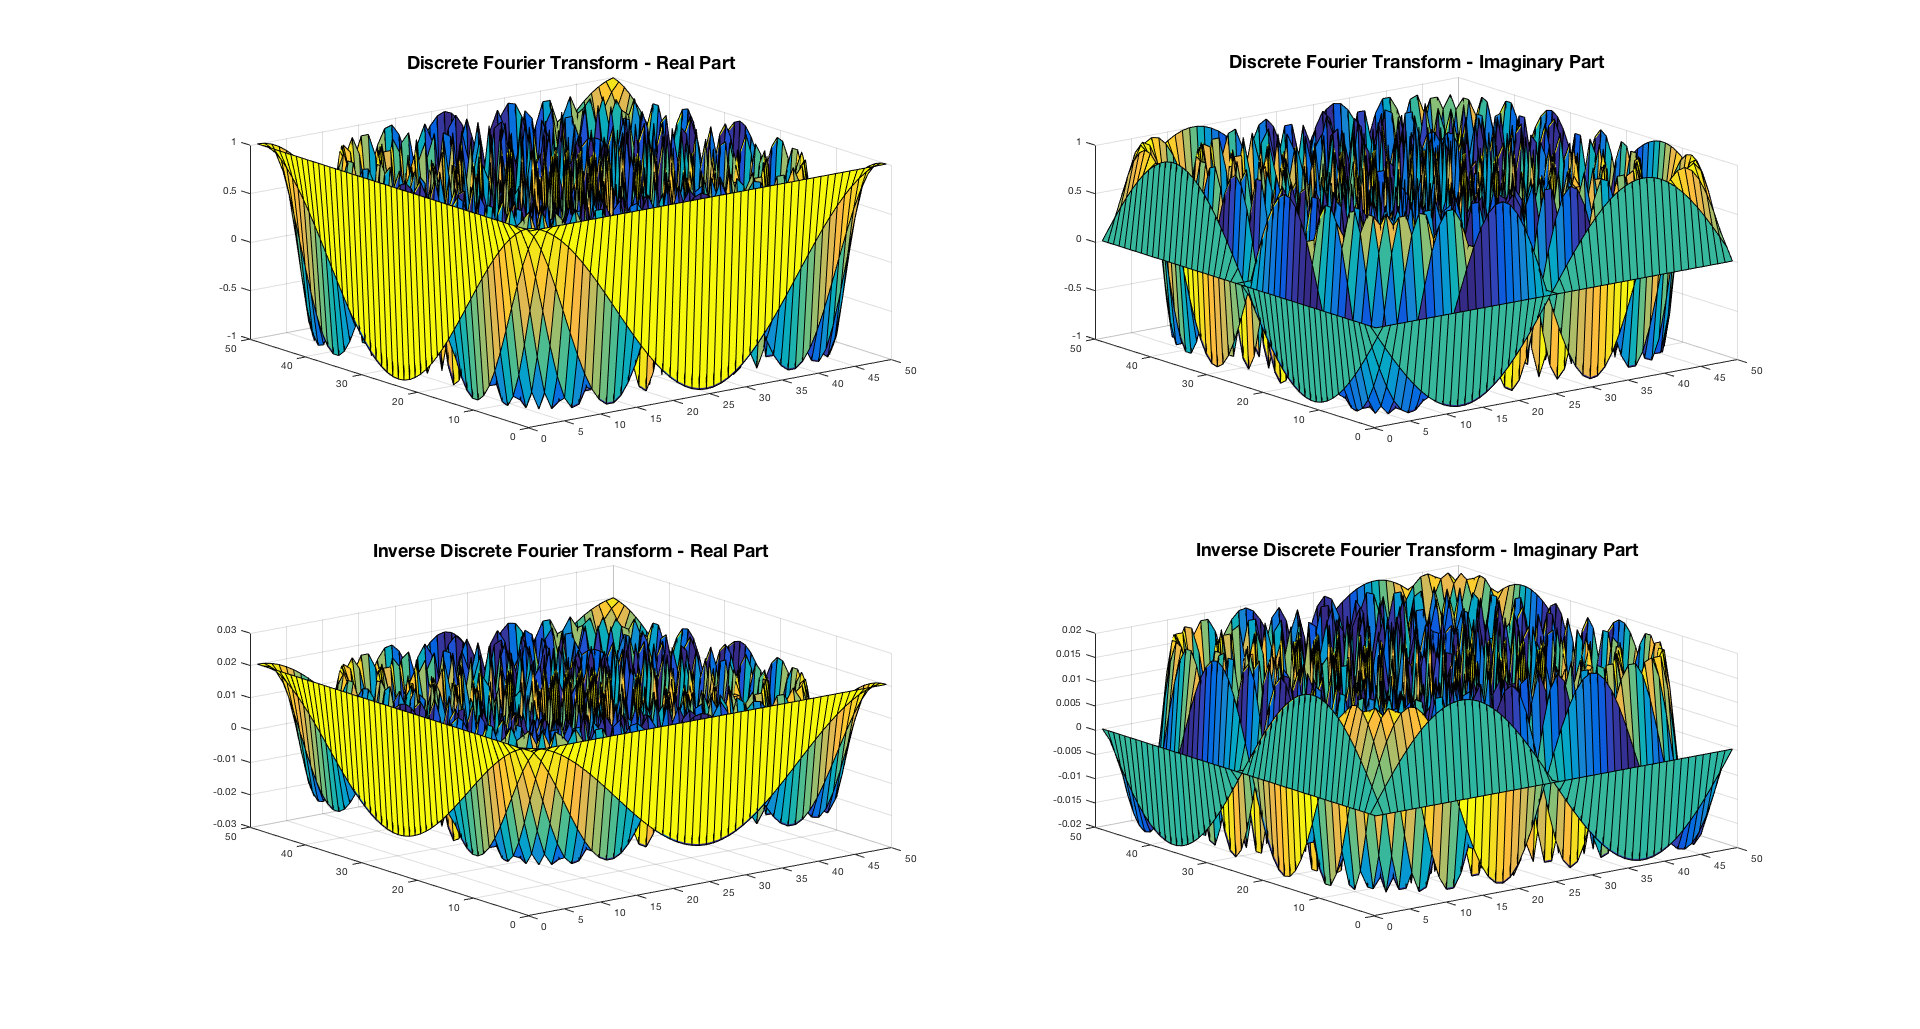
\includegraphics[scale=.22]{Images/DFTRANDI}
\caption{Discrete Fourier Transform \& Inverse DFT real and imaginary part. The above surface created using the matrix F. The graph is created using Matlab program named mydft.m attached in the Appendix}
\label{fig:DFTRANDI}
\end{figure}

\subsubsection{Inverse Discrete Fourier Transform}
The inverse transform of Discrete Fourier Transform is given by

\begin{equation}
f(t) = \frac{1}{N}\sum_{k=0}^{N-1} F(k) e^{j\frac{2\pi}{N} tk }
\end{equation}
The matrix-vector format of the Inverse Discrete Fourier Transform are given by

$\underbrace{
\begin{bmatrix}
f(0) \\
f(1) \\
f(2) \\
\vdots \\
\vdots \\
f(N-1)
\end{bmatrix}}_{\text{Original Signal}}$ \!
= $\frac{1}{N}$
$\underbrace{
\begin{bmatrix}
1 & 1 & \cdots & \cdots & 1 \\
1 & e^{j(\frac{2\pi}{N})} & e^{j(\frac{4\pi}{N})}\cdots & \cdots & e^{j(\frac{2(N-1)\pi}{N}} \\
1 & e^{j(\frac{4\pi}{N})} & e^{j(\frac{8\pi}{N})}\cdots & \cdots &  e^{j(\frac{4(N-1)\pi}{N}} \\
\vdots & & & \vdots \\
\vdots & & & \vdots \\
1 & e^{j(\frac{2(N-1)\pi}{N})} & e^{j(\frac{4(N-1)\pi}{N})}\cdots & \cdots & e^{j(\frac{2(N-1)(N-1)\pi}{N}}) \\
\end{bmatrix} }_{\text{Inverse DFT Matrix:G}}$
$\underbrace{
\begin{bmatrix}
F(0) \\ F(1) \\ F(2) \\ \vdots \\ \vdots \\ F(N-1) 
\end{bmatrix}}_{\text{DFT Vector}}$

The inverse DFT matrix G is inverse of matrix F and scaled by a factor of $\frac{1}{N}$. $G * F = F * G = I$, where as I is an identify matrix of order N. 

\subsection{Short Time Fourier Transformation}
 One of the ideas is to chop the signal into smaller pieces and perform Fourier transformation for each piece. This technique is called short time Fourier Transform. The smaller pieces in the signal can be chosen by a window function $w(t-\tau)$
 \begin{equation}
F(\tau,s) = \int_{-\infty}^{\infty}{f(t)w(t-\tau)e^{-j2\pi t s }dt}
\end{equation}
$w(t)$ represents a window function and there are multiple window functions available to choose. 

\subsubsection{Gaussian Window}
The Gaussian Window is defined as 
\begin{equation}
w(n) = e^\frac{-(n-m)^2}{2(\sigma N)^2}
\end{equation}
for $n = 0,1,2,... N-1$,where $N$ is the length of the window, $m=\frac{(N-1)}{2.0}$, and the $\sigma$ is the standard deviation of the Gaussian window. The Gaussian window is useful for time-frequency analysis because the Fourier transform and the derivate of a Gaussian window both are Gaussian function.

\subsubsection{Hamming Window}
The Hamming window is defined as 
 \begin{equation}
w(n) = \alpha - \beta \cos(\frac{2\pi n}{N - 1})
\end{equation}
where the constants $\alpha$ and $\beta$ are approximations to the values of $\frac{25}{46}$ and $\frac{21}{46}$ respectively. The values of $\alpha$ and $\beta$ are given as $0.54$ and $0.46$ respectively. 

 \begin{equation}
w(n) = 0.54 - 0.46 \cos(\frac{2\pi n}{N - 1}), 0 \le n \le N
\end{equation}
The window length is $L = N + 1$.

\begin{figure}[!ht]
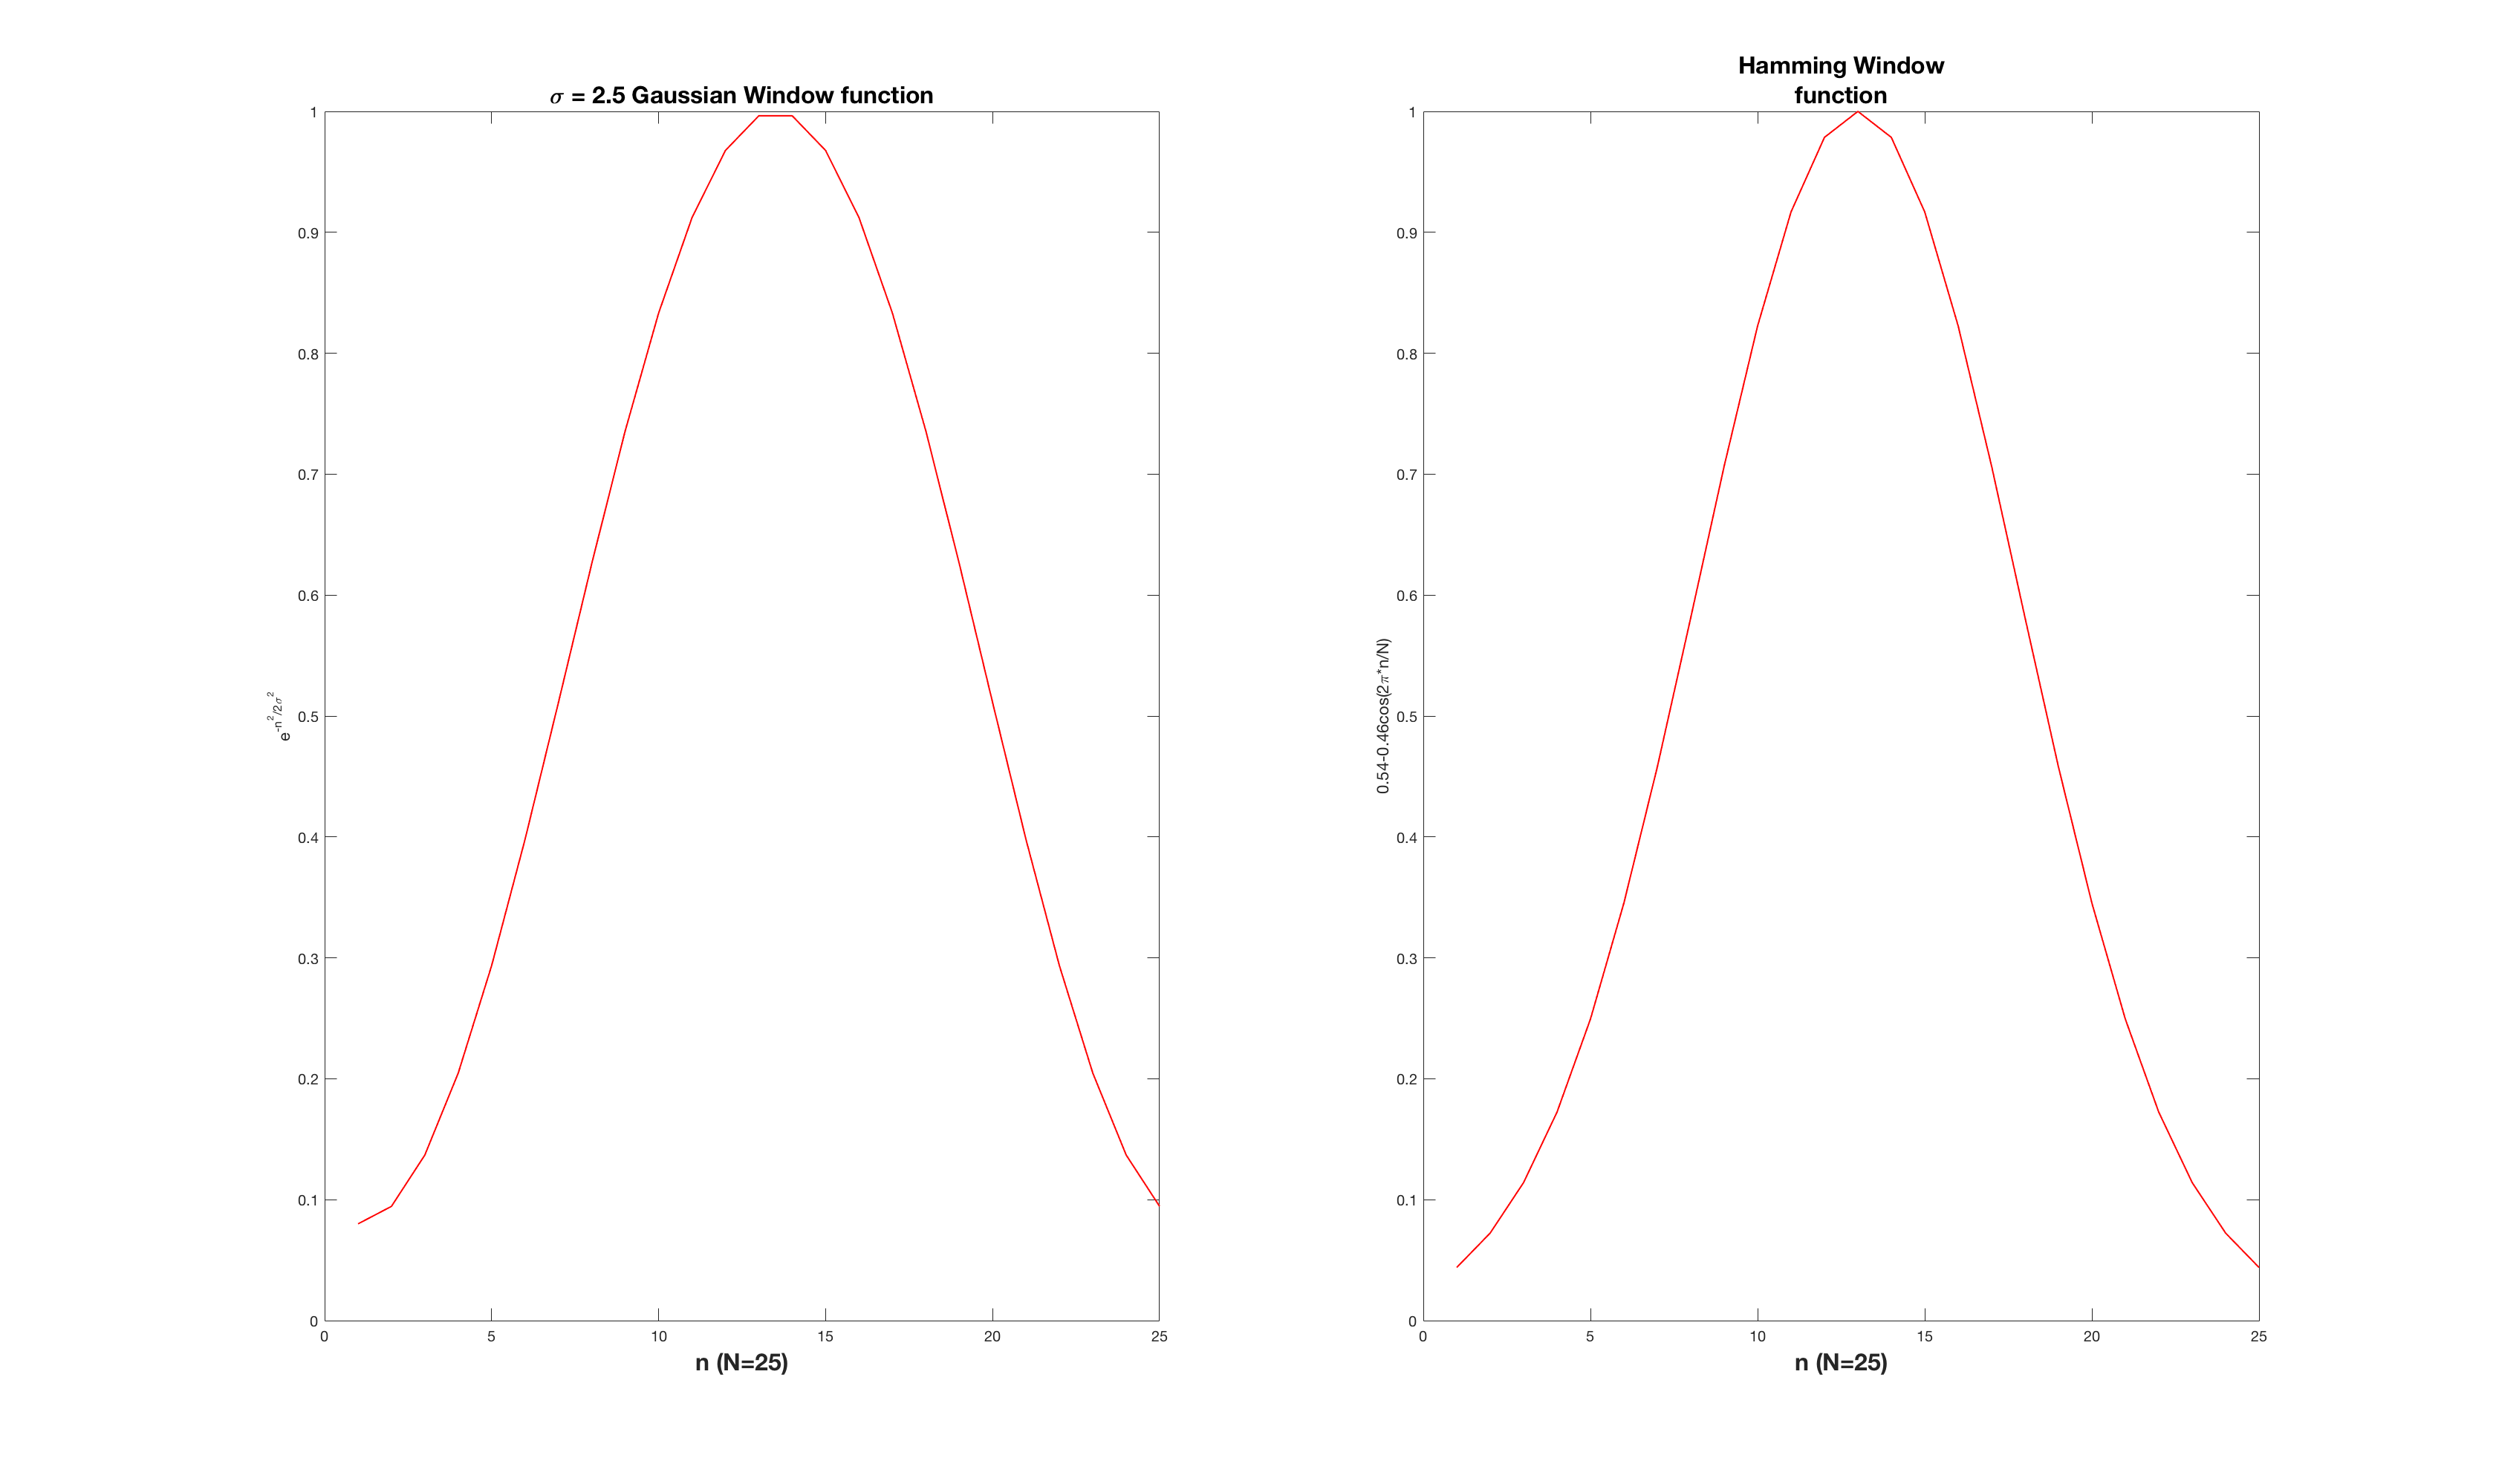
\includegraphics[scale=.15]{Images/GWinHWin}
\caption{Window function (window length  =25) for a) Gaussian b) Hamming. The graph was created using Matlab program ghamwin.m and attached in Appendix B }
\label{fig:ghamwin}
\end{figure}

The short time Fourier transform is performed for several signals using Hamming and Gaussian windows and the results are given below.

The first signal is

\begin{equation}\label{pwise}
f(t)  =
\left\{
\!
\begin{aligned}
sin(2\pi 300 t)  & \quad \quad \text{ if }\quad 0< t<\frac{T}{3}\\
sin(2\pi 200 t)  & \quad \quad \text{ if }\quad \frac{T}{3}+1<t<\frac{2T}{3}\\
sin(2\pi 100 t)  & \quad \quad \text{ if }\quad  \frac{2T}{3}+1<t<T
\end{aligned}
\right.
\end{equation}
Where T is the complete duration of $f(t)$. Operations like Fourier Transformation, Short Time Fourier Transform (STFT), STFT with Gaussian and Hamming windows are performed for the function given in \ref{pwise} and results of it is compared with similar operations for the SP500 Cycles, NASDAQ Cycles and results are given in Figure \ref{pwise}

\begin{figure}[!ht]
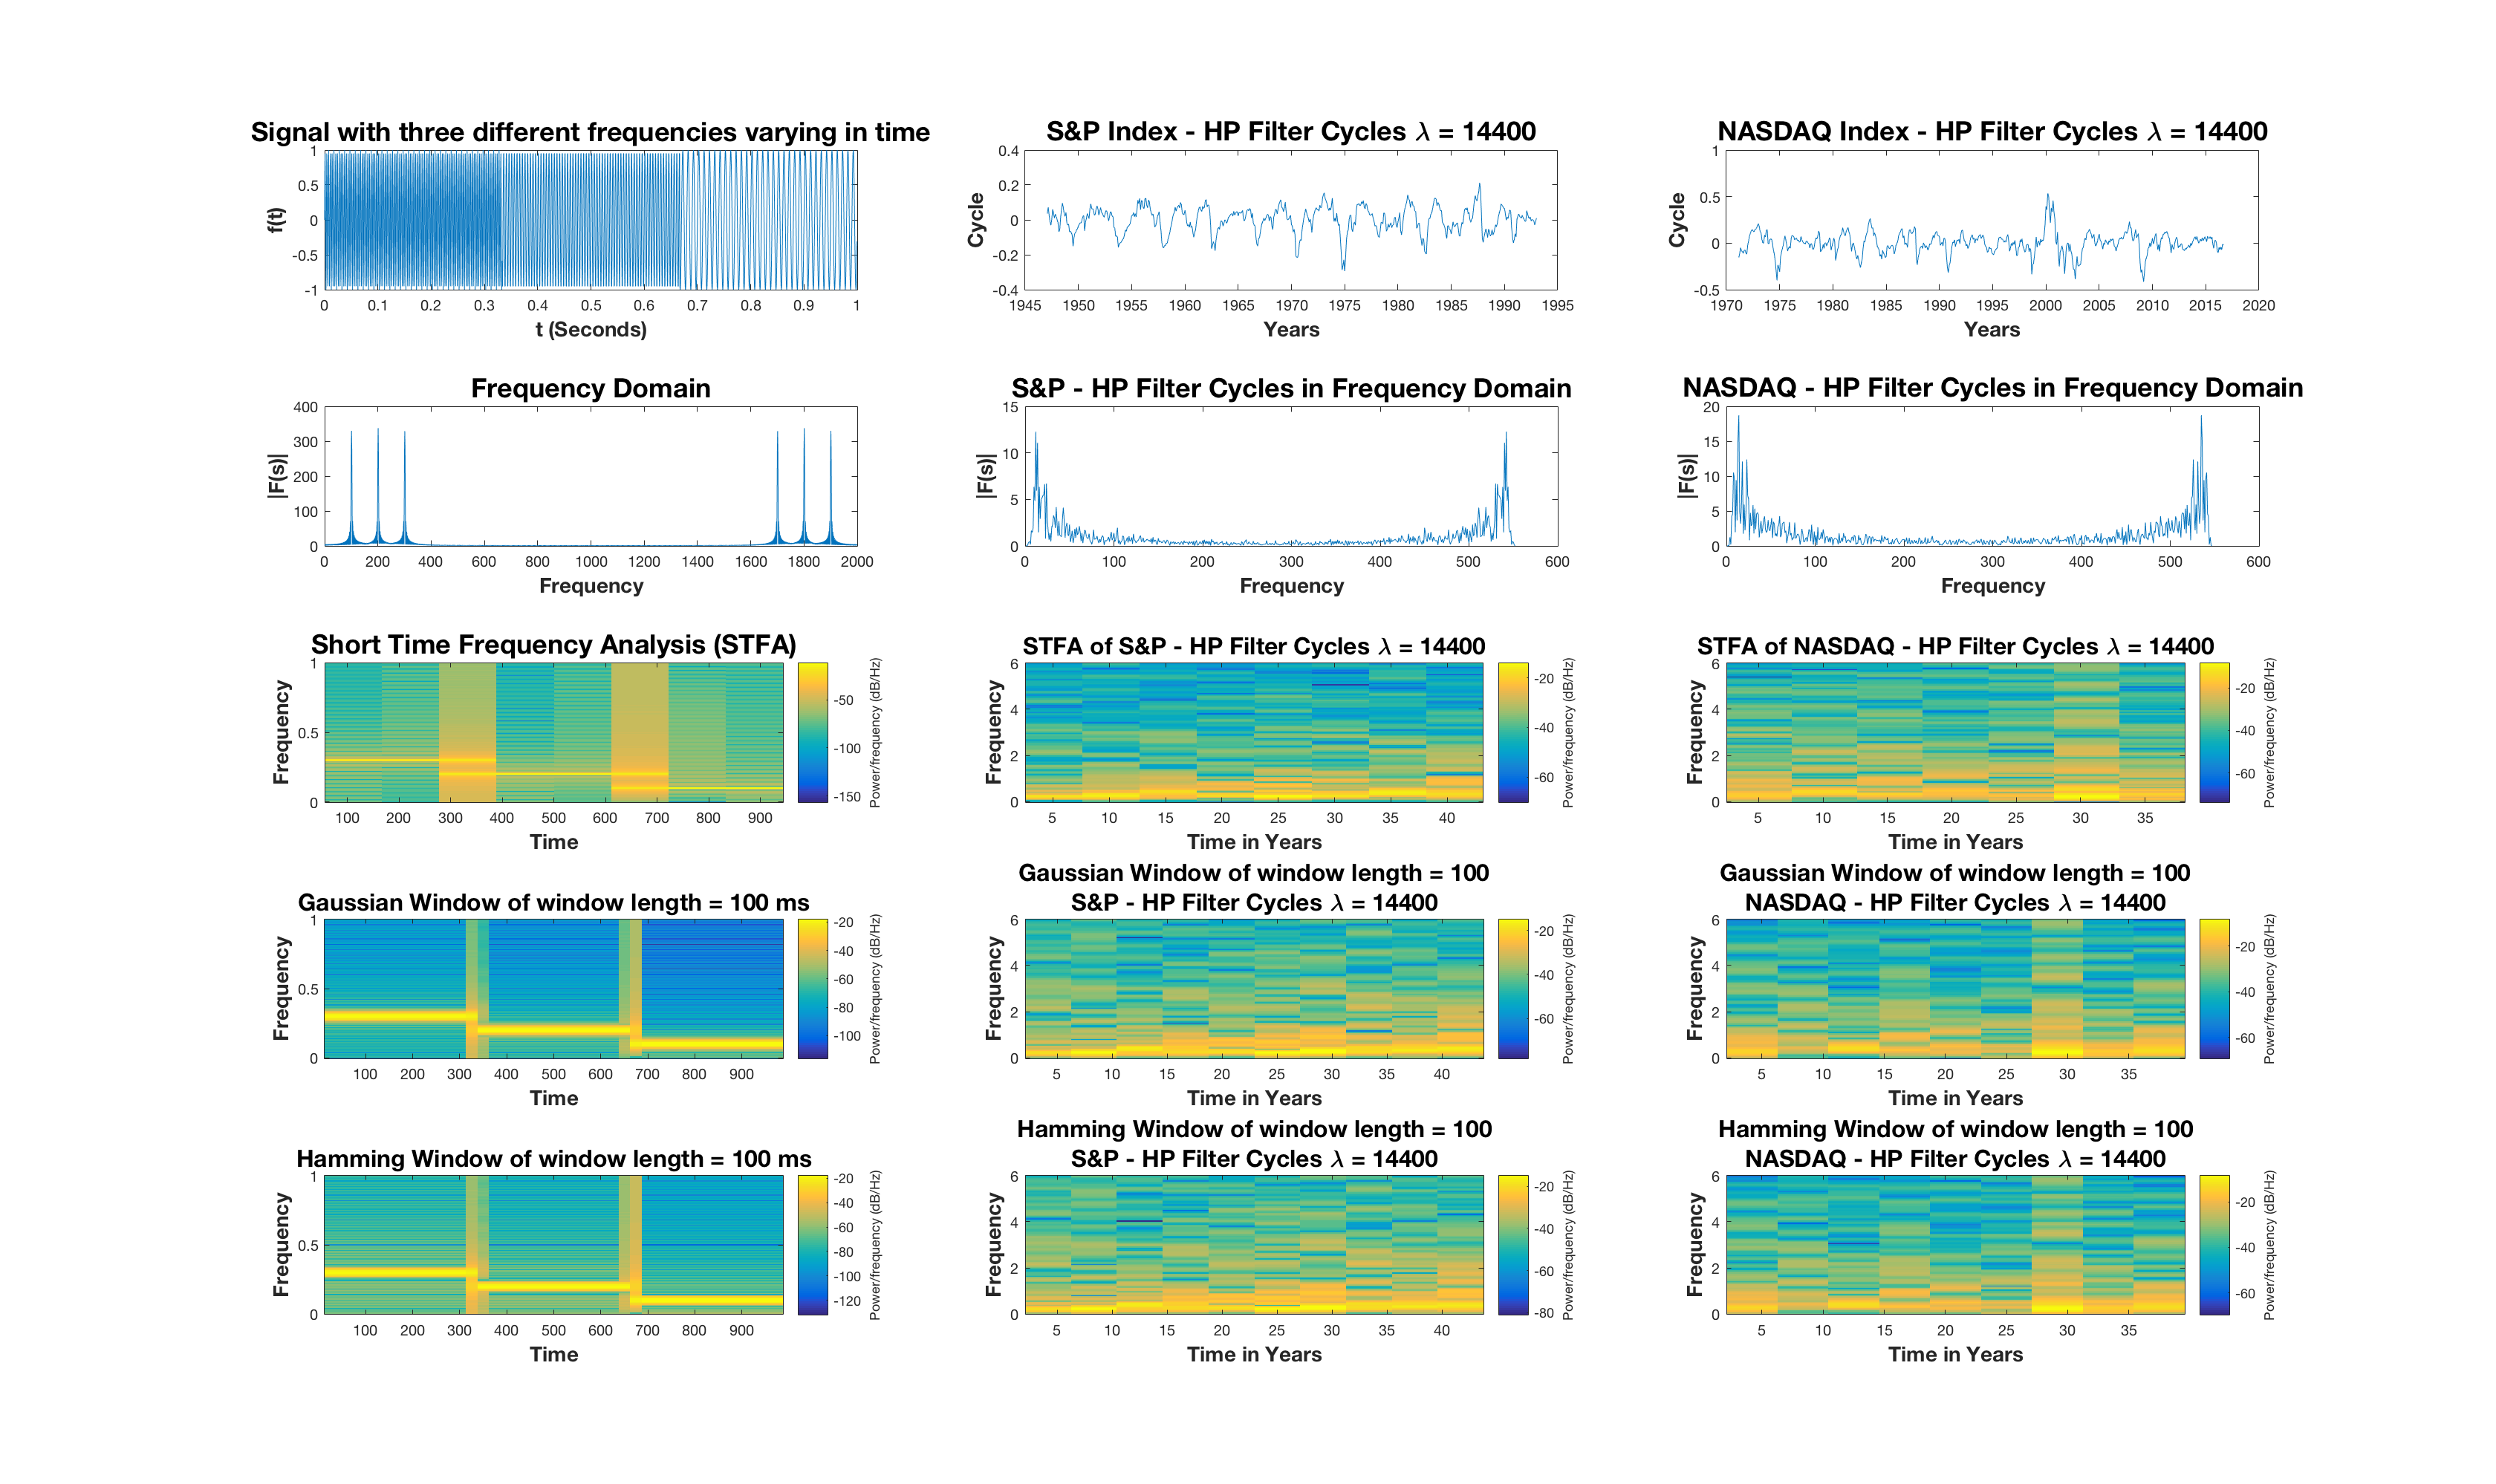
\includegraphics[scale=.16]{Images/Spectrum}
\caption{In the first column, the signal $f(t)$ as defined in \ref{pwise} b) Fourier Transform of $f(t)$ c) Short Time Fourier Transform of $f(t)$ d) STFT using Gaussian window e) STFT using Hamming window. Second column is for SP500 and third column is for NASDAQ indexes. The graph was created using Matlab program spectrumAnalysis5.m and attached in Appendix B }
\label{fig:spectrum}
\end{figure}


Simultaneous analysis of signals in both time and frequency domains provides better understanding of the signal and the short time Fourier transform laid the foundation for the joint time-frequency analysis.
\section{Introduction to Gabor Transformation}
The Gabor transformation or expansion in signal synthesis uses the Gabor elementary function (GEF) as the base function (equivalent of simple harmonic function in the Fourier transform) and the idea was influenced by Heisenberg's uncertainty principle.  \\
\subsection{Heisenberg's uncertainty principle}
In quantum mechanics, simultaneously, both the position of a particle and the momentum of the particle can not be measured preciously. Let $x$ be position and $p$ be momentum of the particle. The standard deviation of $x$ and $p$ are denoted by $\Delta x$ and $\Delta p$ respectively. The uncertainty principle states that product of the standard deviations of position and momentum is greater than or equal to $\frac{\hbar}{2}$
\begin{equation*}
\Delta x\Delta p \geq \frac{\hbar}{2}
\end{equation*}
\begin{equation*}
\begin{split}
\Delta x &= \sqrt{\langle(x - \langle x\rangle)^2\rangle} \\
\Delta p &= \sqrt{\langle(p - \langle p \rangle)^2\rangle}
\end{split}
\end{equation*}

\begin{comment}
\begin{equation*}
\Delta p = \sqrt{\langle(p - \langle p \rangle)^2\rangle}
\end{equation*}
\end{comment}

\subsection{Gabor Transformation }
Gabor had the insight that the base function with minimum uncertainty in both time and frequency domains best captures temporal information during the frequency analysis.

Gabor in his original study proposed an elementary function in complex form which occupies minimum uncertainty and it is a product of harmonic oscillator of any frequency and a Gaussian function. The area occupied by the following elementary function in the joint time frequency domain is equal to the minimum uncertainty.

\begin{equation}
\zeta(t) = \underbrace{e^{-\alpha ^2(t)^2}}_v\overbrace{e^{j2\pi f_0 t+\phi}}^w
\end{equation}

An arbitrary function $f(t)$ can be represented by a series of elementary functions which are constructed by translation in both the time and frequency domains. The function $f(t)$ is synthesized by the combination of GEFs.\\

\begin{equation}\label{gcoff}
f(t) = \sum_{m,n\in Z} C_{m,n} \psi_{m,n}(t)
\end{equation}
where the $C_{m,n}$ are Gabor coefficients and the $\psi_{m,n}(t)$ are the bases functions called Gabor elementary functions. A GEF translated by 'na' is denoted by $\psi_n$ and given by
\begin{equation*}
\psi_{n}(t) = \psi(t-na)\\
\end{equation*}
The translation in the frequency domain is also called modulation. A GEF is modulated by using simple harmonic functions. 
\begin{equation*}
\psi_{m,n}(t) = \psi(t-ma) e^{j2\pi nbt}
\end{equation*}\\
The original Gabor paper suggested that $\psi$ is Gaussian. GEFs were studied by using other functions for $\psi$ like a rectangle.  a and b are time and frequency shift parameters and a,b $>$  0. $\psi_{m,n}$ is obtained by shifting it by  ma $\times$ nb in the time-frequency plane.\\

For the given data set of NASDAQ and SP500 indexes data, the shift is towards a discrete time signal that is sampled for a finite time. Recalling \ref{gcoff}, 
\begin{equation}\label{gcoff1}
f(t) = \sum_{m=0}^{M-1}\sum_{n=0}^{N-1} C_{m,n} \psi_{m,n}(t)
\end{equation}
where $\psi_{m,n}(t)$ is Gabor Elementary functions.
$C_{m,n}$ is calculated as follows
\begin{equation}\label{cmn}
C_{m,n}  = \sum_t f(t) h(t-m\Delta M) e^\frac{-j2\pi t n\Delta N}{N}
\end{equation}
where $h$ is an analysis window.
$\Delta M$, $\Delta N$ are time and frequency sampling intervals respectively. $M$, $N$ are the number of sampling points in time and frequency domains. $\Delta M$, $\Delta N$, $M$, $N$ are chosen to meet the sampling criteria, $M\Delta M = L$ and $N\Delta N = L$. 


\begin{figure}[!ht]
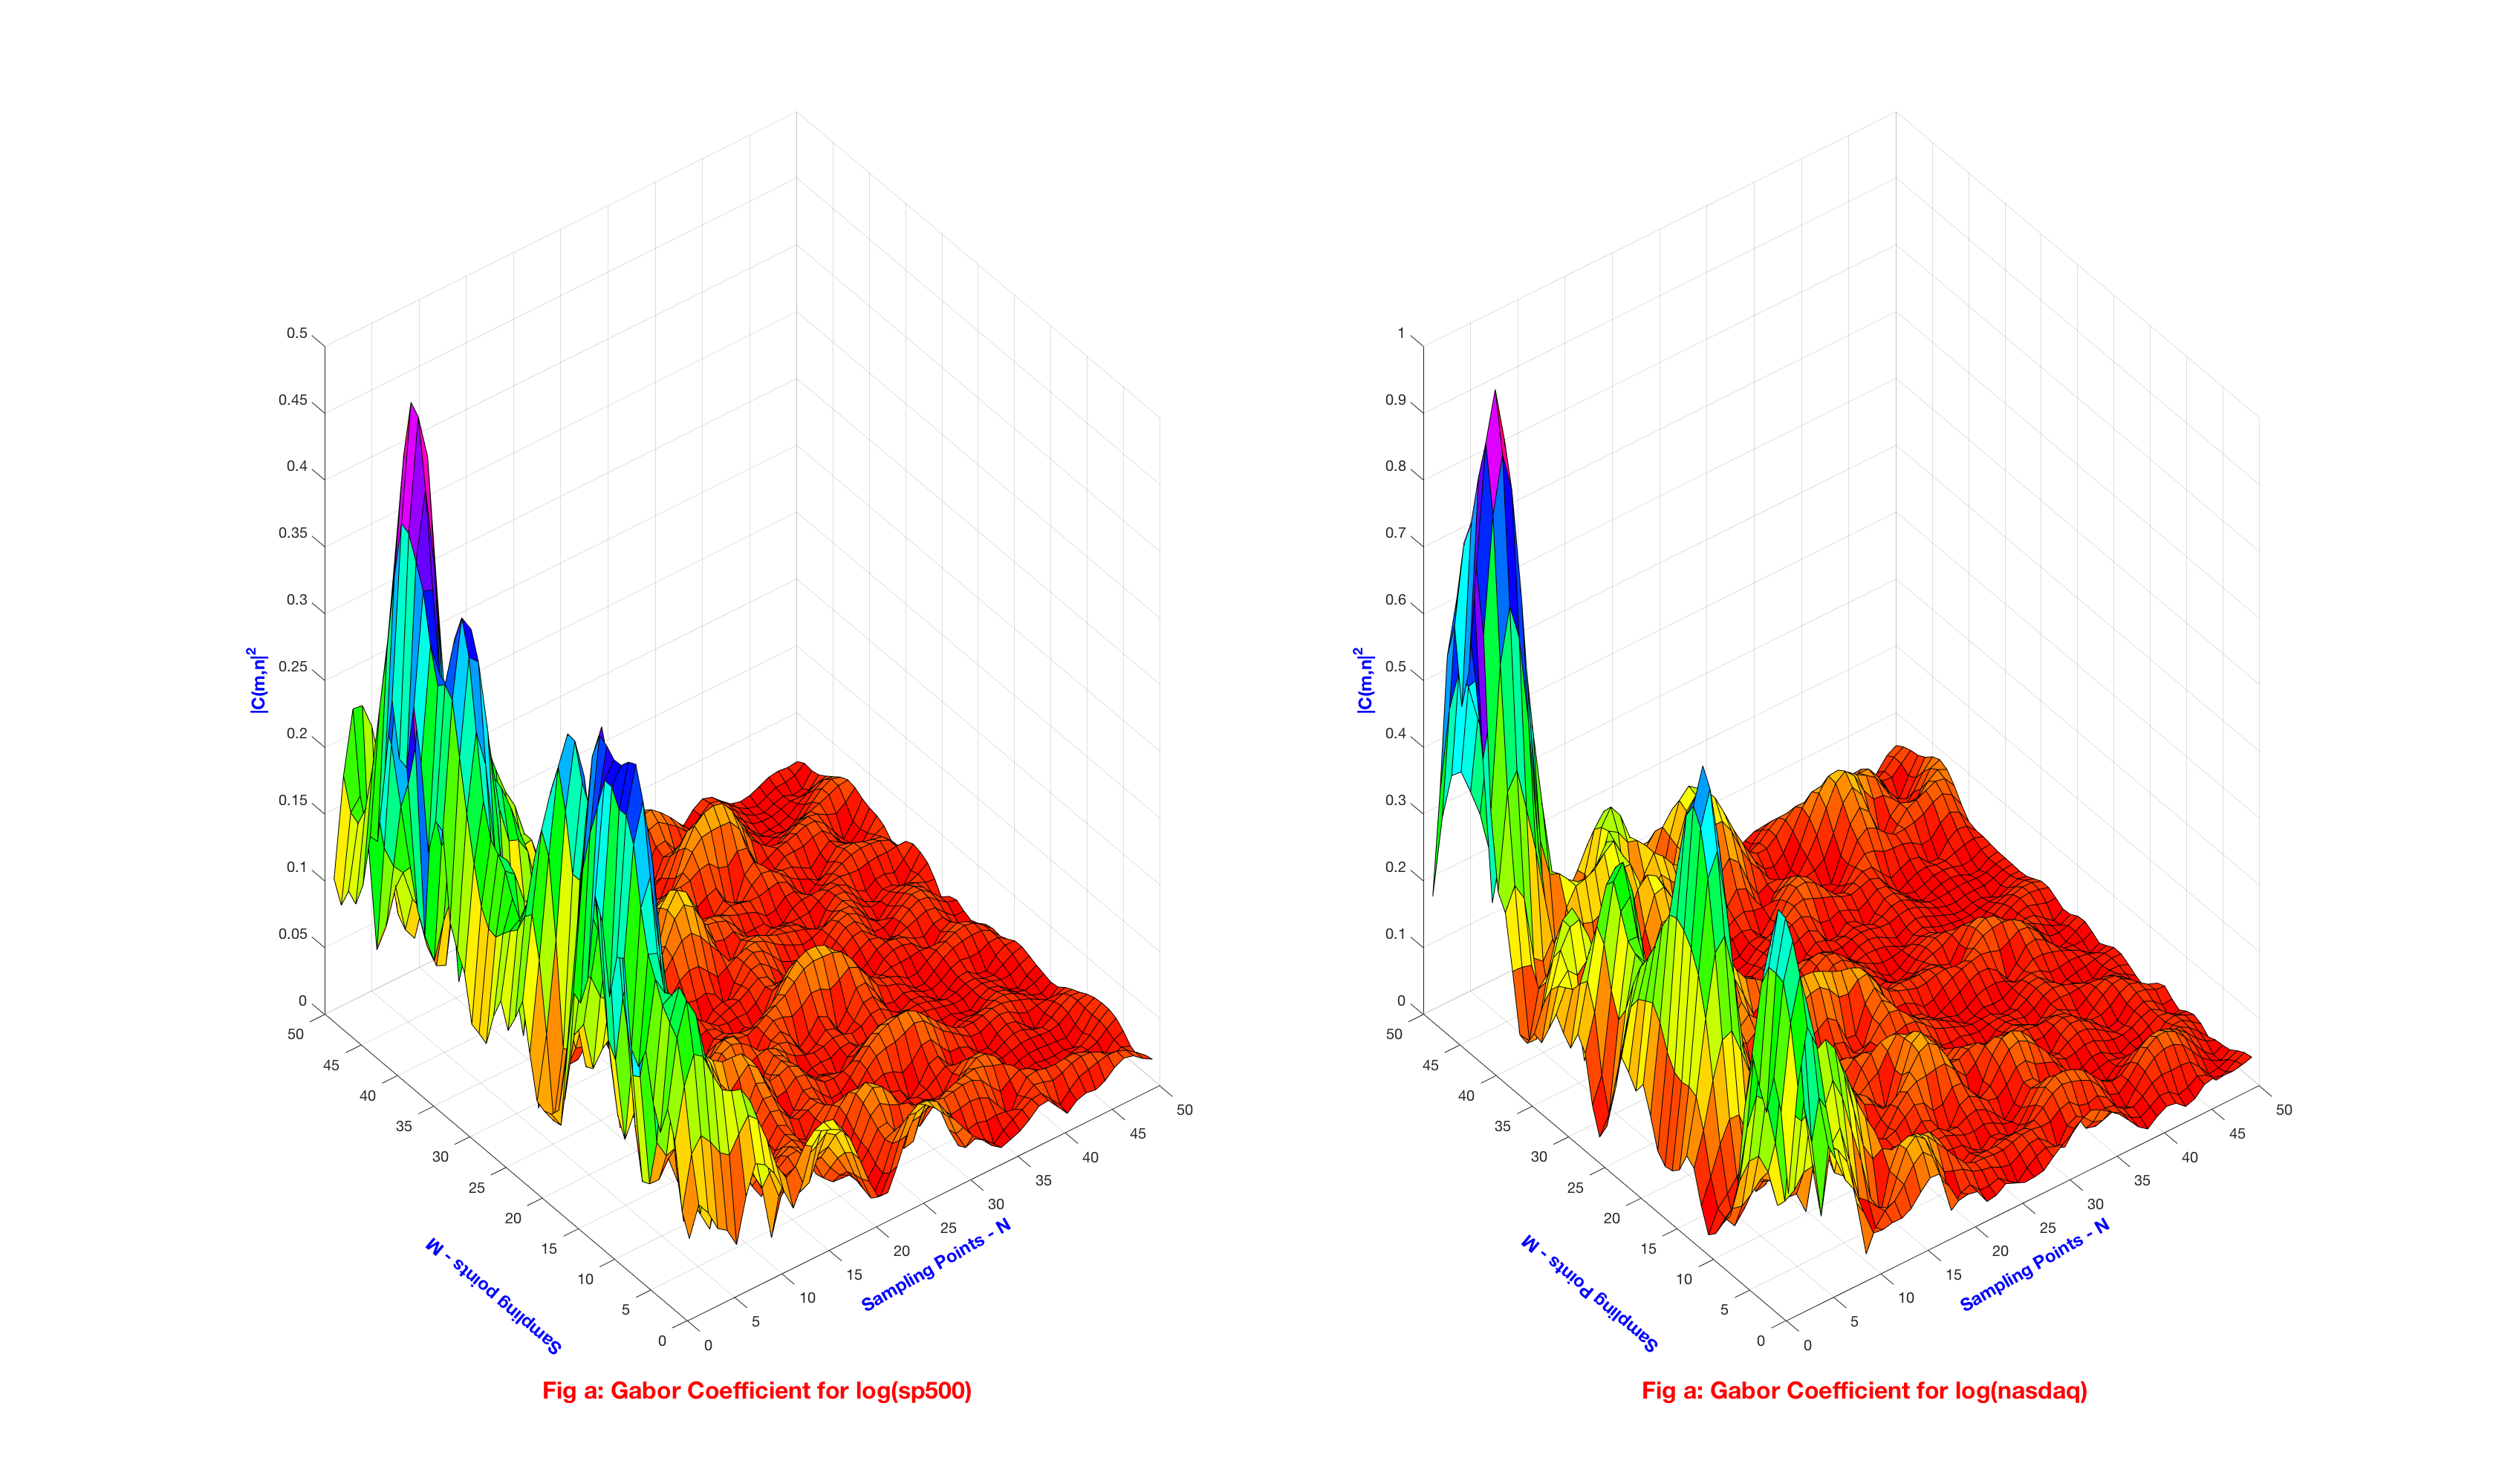
\includegraphics[scale=.15]{Images/GaborThreshold50}
\caption{Fig a is the time section of Gabor distribution of HP Filter cycles log(SP500) and Fig b is the time section of Gabor distribution of for HP Filter cycles log(NASDAQ). $\Delta M = 8; \Delta N = 4; m = 50; n = 100; \sigma = \sqrt{\frac{\Delta M L}{\Delta N 2\pi}}$. Threshold is calculated as $max(|c(m,n)|-min(|c(m,n)|))/2$. The program used to create the graph is mygaborfilt.m and it is attached in the appendix.}
\label{fig:GaborThreshold50}
\end{figure}

\begin{figure}[!ht]
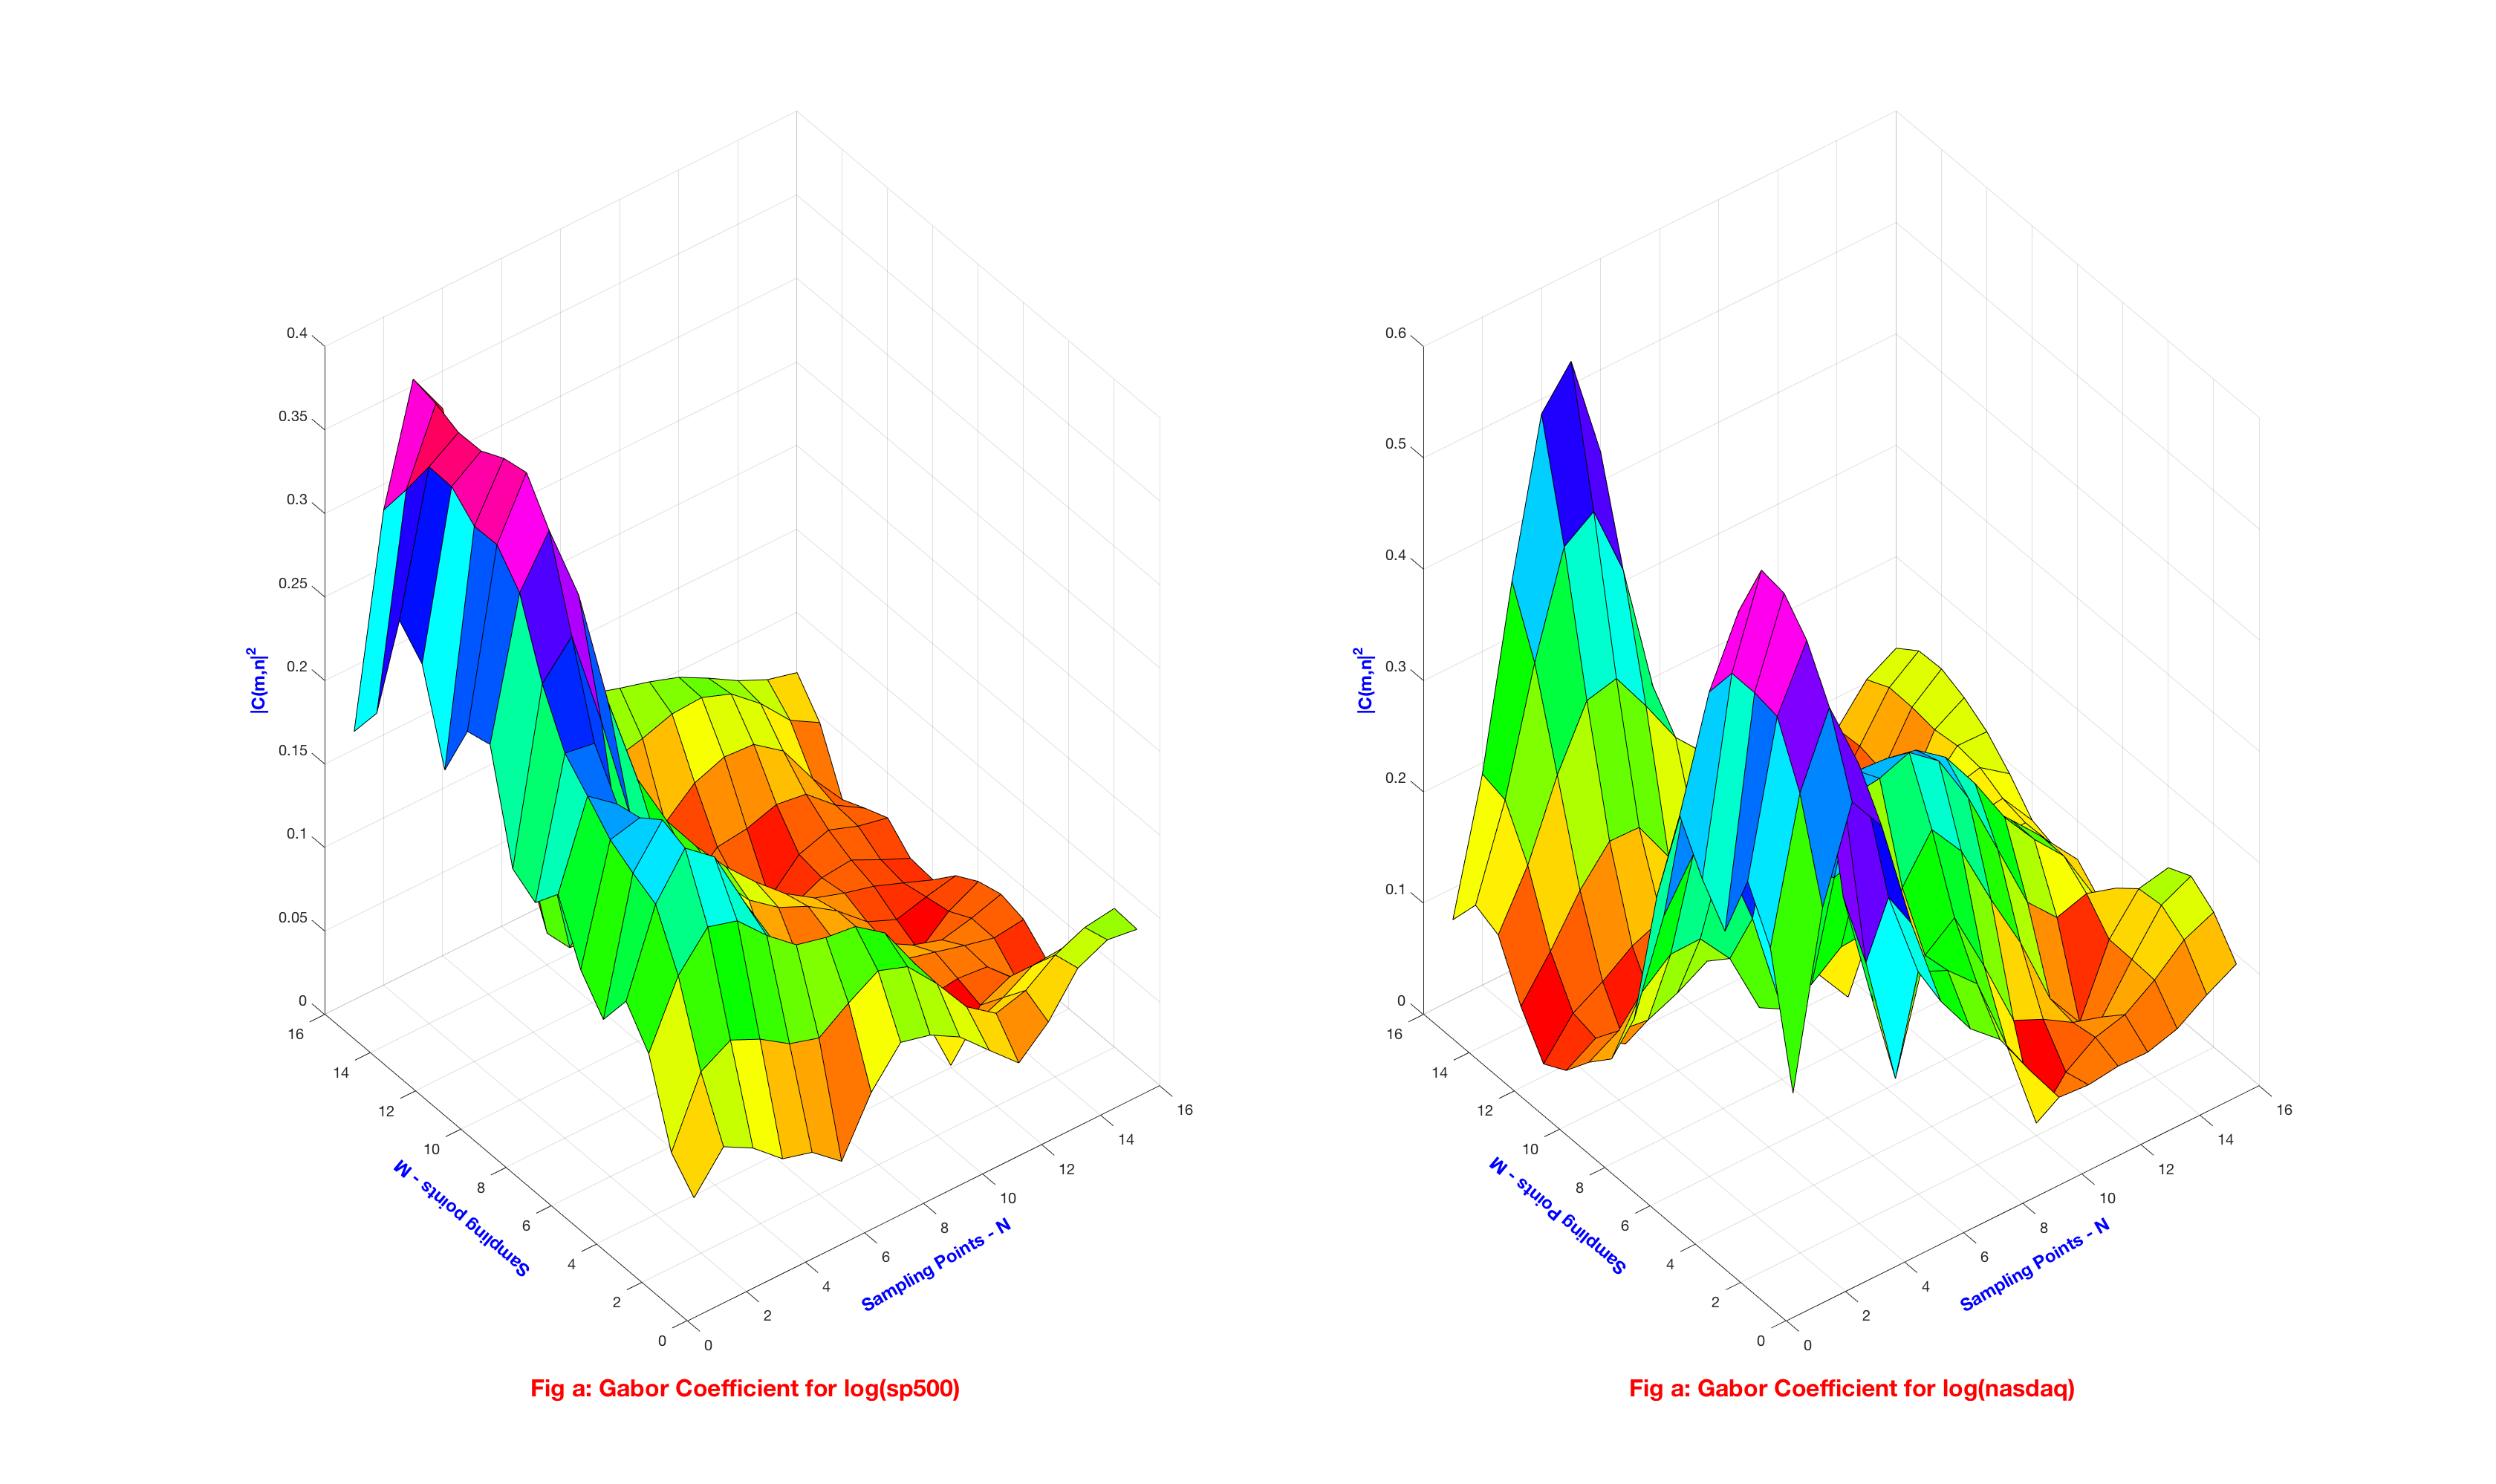
\includegraphics[scale=.15]{Images/GaborThreshold16}
\caption{Fig a is the time section of Gabor distribution of HP Filter cycles log(SP500) and Fig b is the time section of Gabor distribution of for HP Filter cycles log(NASDAQ). $\Delta M = 8; \Delta N = 4; m = 16; n = 32; \sigma = \sqrt{\frac{\Delta M L}{\Delta N 2\pi}}$. Threshold is calculated as $max(|c(m,n)|-min(|c(m,n)|))/2$. The program used to create the graph is mygabor.m and it is attached in the appendix.}
\label{fig:GaborThreshold16}
\end{figure}


\begin{comment}
Gabor co-efficient $C_{m,n}$ and synthesis function $f(t)$ are bi-orthogonal functional sets.  \\
\begin{equation}
C_{m,n} = \sum_{m,n\in Z} \psi_{m,n}^*(t) f(t)
\end{equation}
$\psi_{m,n}^*$ is the complex conjugate of $\psi_{m,n}$.\\
\\
\end{comment}
The GEFs could be a set of Gaussian functions modulated by simple harmonics. GEFs are generated in 1D by combining Gaussian and simple harmonic functions. The Gaussian function remained the same for both GEF and only the sinusoidal functions changed between the two GEFs. Note the change in the frequency between the GEFs. A set of GEFs can be created by varying ma and nb.\\
\begin{equation*}
\psi_{m,n}(t) =  e^{-\frac{(t-\mu-ma)^2}{2\sigma^2}} e^{j2\pi nbt}
\end{equation*}

If the GEF $\psi$ and its Fourier transform (frequency representation) $\Psi$ are localized at the origin then $\psi_{m,n}$ is localized at (ma,nb) in the joint time-frequency domain. Each GEF occupies a region in time-frequency plane and associated $C_{m,n}$ represents a quantum of information.\\

Let $\psi(t)$ be a GEF. The GEF in the frequency domain is given by the Fourier transform \\
\begin{equation*}
\Psi(f) = \int_{-\infty}^{\infty}\psi(t) e^{-j2\pi ft}\, dt \\
\end{equation*}

These functions have a special property that relates to Heisenberg's uncertainty principle. The product of the standard deviation in time $\Delta t$ and variance in frequency $\Delta f$ is always greater than or equal to a certain quantity.
\begin{equation}
\Delta f \Delta t \geq \frac{1}{4\pi}
\end{equation}
The time standard deviation or effective duration and frequency variance or effective frequency width can be calculated by the root mean square (RMS) deviation of the signal from the mean. The effective duration ($\Delta t$) and effective frequency width ($\Delta f$) are given by
\begin{equation*}
\Delta t = \sqrt{\frac{\int_{-\infty}^{\infty}{\psi(t)(\mu_t - t)^2\psi ^*(t)dt}}{\int_{-\infty}^{\infty}{\psi(t)\psi ^*(t)dt}}} ;
\Delta f = \sqrt{\frac{\int_{-\infty}^{\infty}{\Psi(f)(\mu_f - f)^2\Psi ^*(f)df}}{\int_{-\infty}^{\infty}{\Psi(f)\Psi ^*(f)df}}}
\end{equation*}

where $\mu_t$ and $\mu_f$ are mean time and mean frequency and they are given by
\begin{equation*}
\mu_t = \frac{\int_{-\infty}^{\infty}{\psi(t)t\psi ^*(t)}}{\int_{-\infty}^{\infty}{\psi(t)\psi ^*(t)}} ;
\mu_f = \frac{\int_{-\infty}^{\infty}{\Psi(f)f\Psi ^*(f)}}{\int_{-\infty}^{\infty}{\Psi(f)\Psi ^*(f)}}
\end{equation*}

\subsection{Mask Operator}
In general, random noise tends to spread evenly in the joint time-frequency domain, while the signal itself concentrates in a relatively small range. Consequently, by a joint time-frequency representation, the signal-to-noise ratio could be substantially improved. Once the interesting signal has been identified, we can apply a mask operator to eliminate the background noise. Typical procedure of the time-variant filter is first to take the Gabor transform and then apply the mask operator to eliminate the background noise to obtain noiseless Gabor coefficients. 

\begin{figure}[!ht]
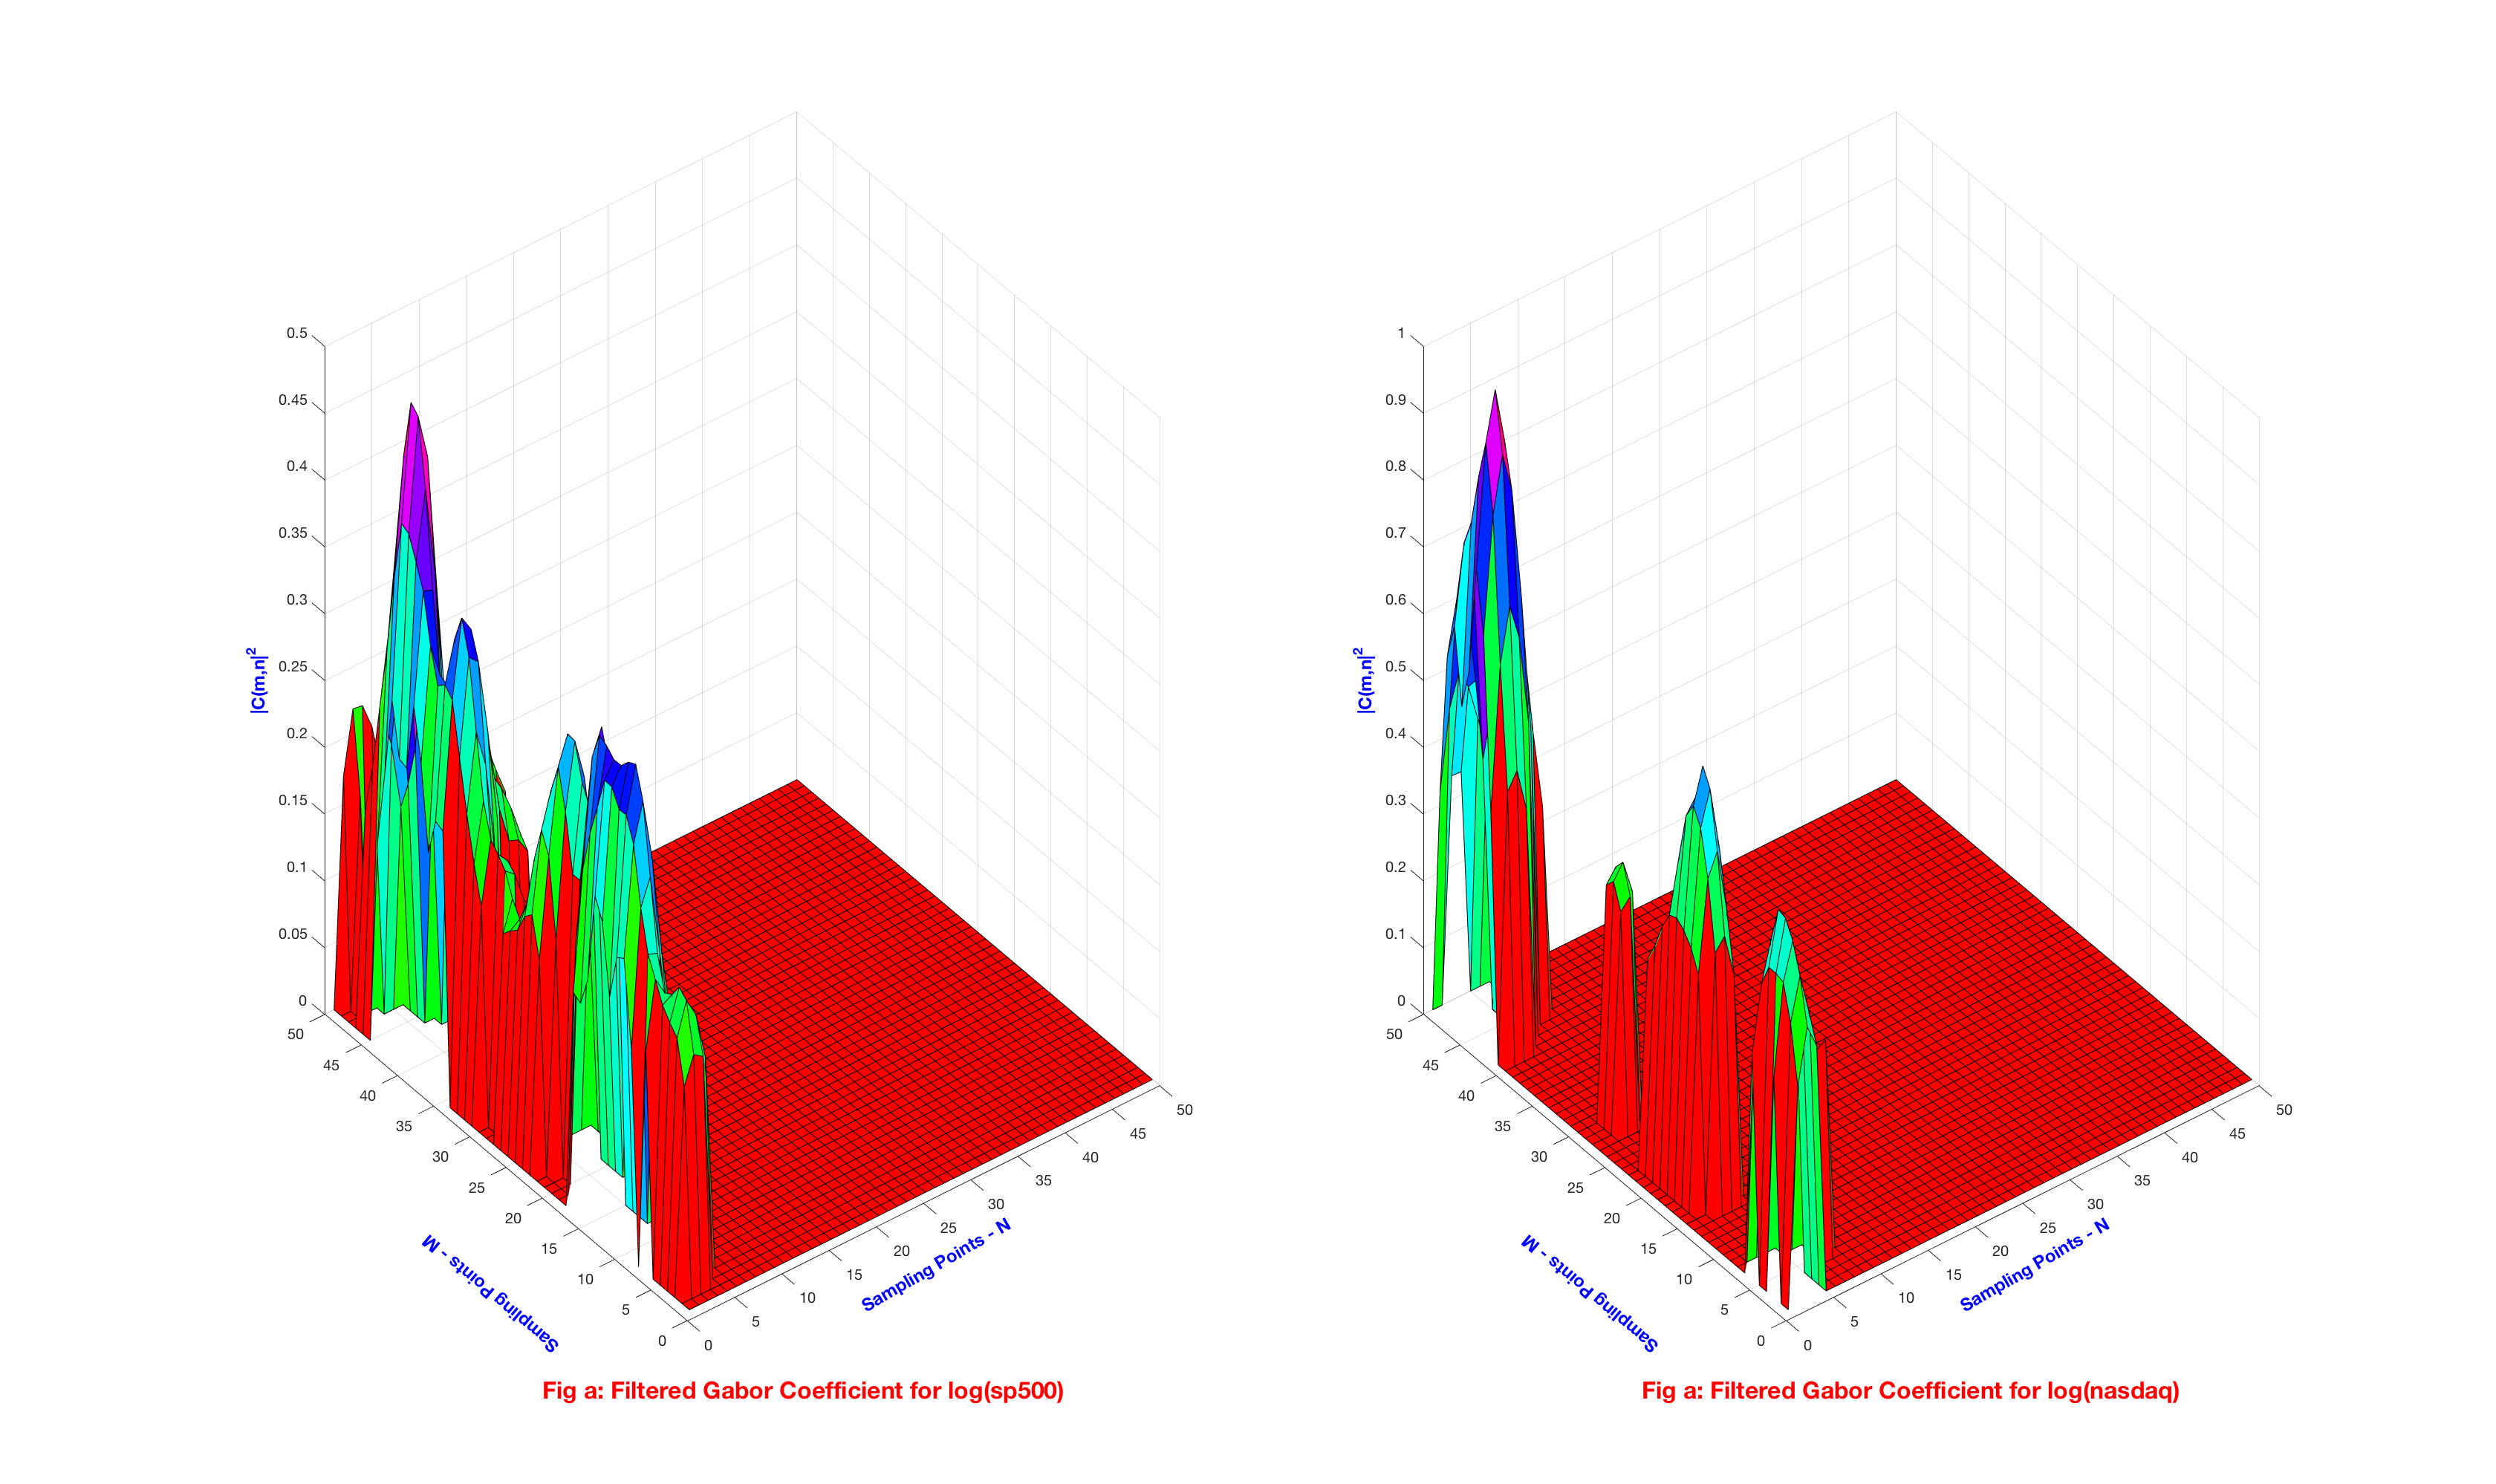
\includegraphics[scale=.15]{Images/GaborMasked50}
\caption{Fig a is the Filtered Gabor Coefficient for HP Filter cycles log(SP500) and Fig b is the Filtered Gabor Coefficient for HP Filter cycles log(NASDAQ).$\Delta M = 8; \Delta N = 4; m = 50; n = 100; \sigma = \sqrt{\frac{\Delta M L}{\Delta N 2\pi}}$. The mask operator is created based on the threshold of a peak distribution. The program used to create the graph is myfiltgabor.m and it is attached in the appendix.}
\label{fig:GaborMasked50}
\end{figure}

\begin{figure}[!ht]
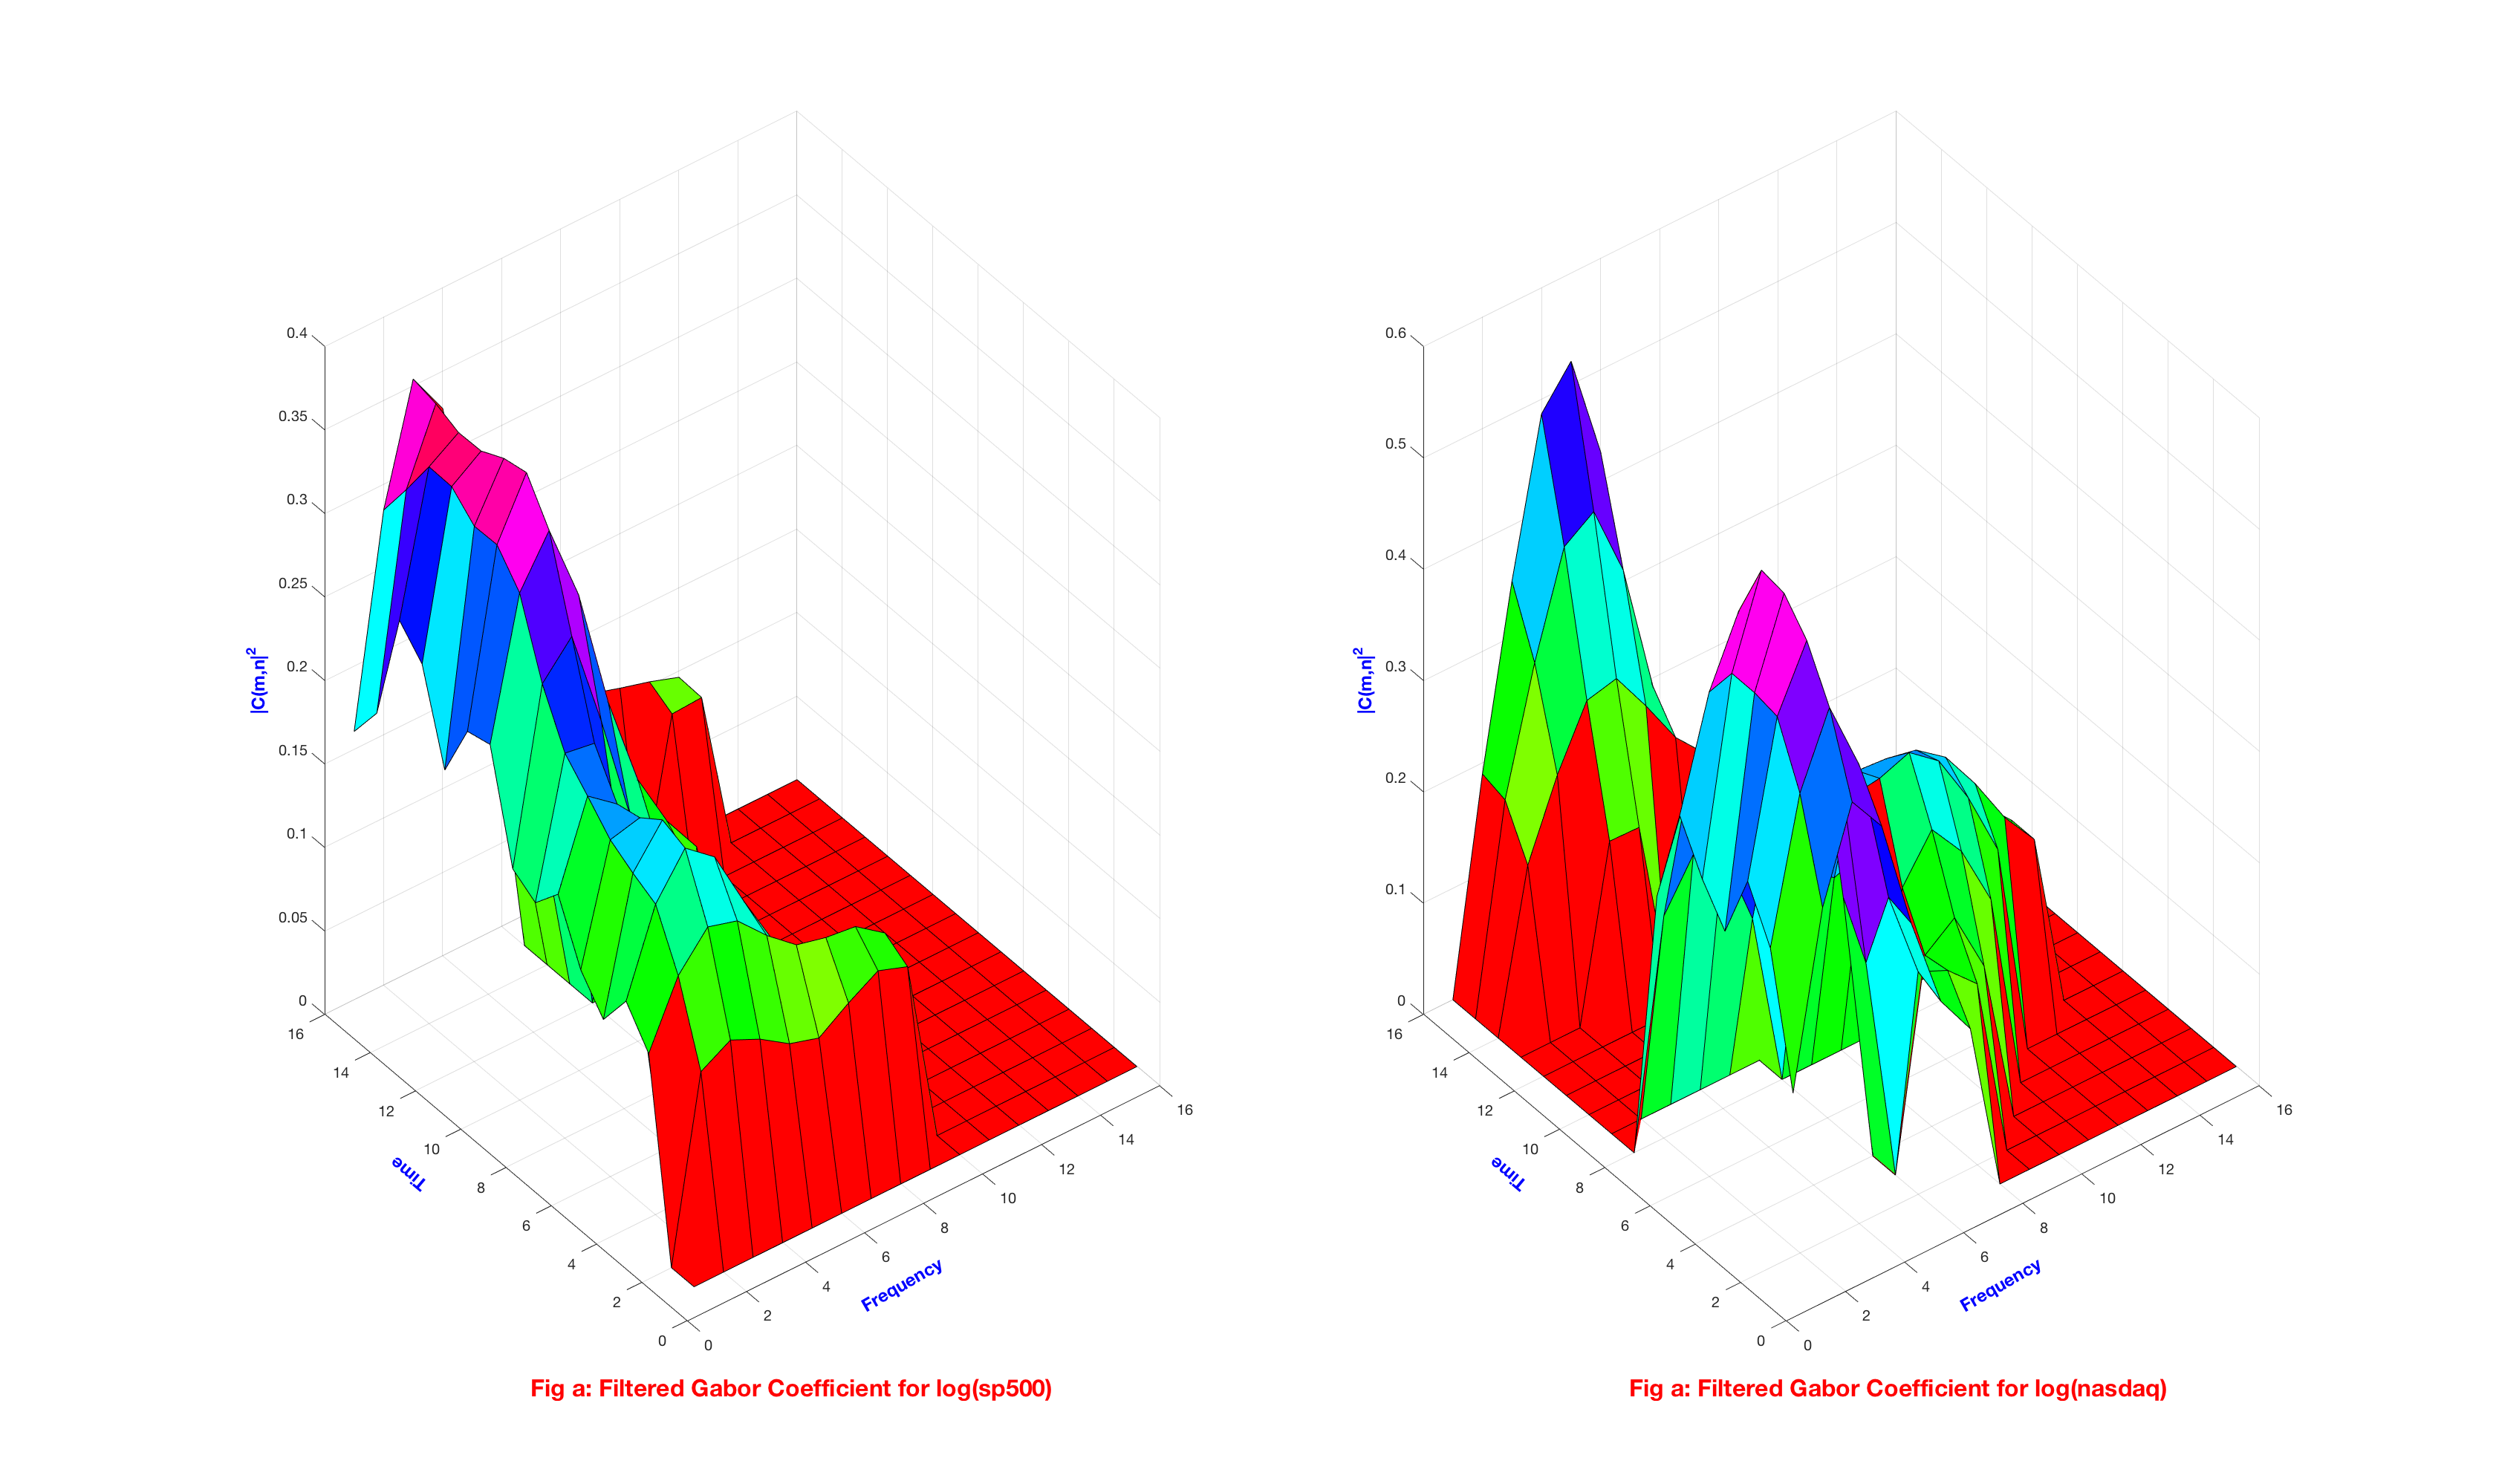
\includegraphics[scale=.15]{Images/GaborMasked16}
\caption{Fig a is the Filtered Gabor Coefficient for HP Filter cycles log(SP500) and Fig b is the Filtered Gabor Coefficient for HP Filter cycles log(NASDAQ).$\Delta M = 8; \Delta N = 4; m = 16 ;n = 32 ; \sigma = \sqrt{\frac{\Delta M L}{\Delta N 2\pi}}$. The mask operator is created based on the threshold of a peak distribution. The program used to create the graph is myfiltgabor.m and it is attached in the appendix.}
\label{fig:GaborMasked16}
\end{figure}

\begin{figure}[!ht]
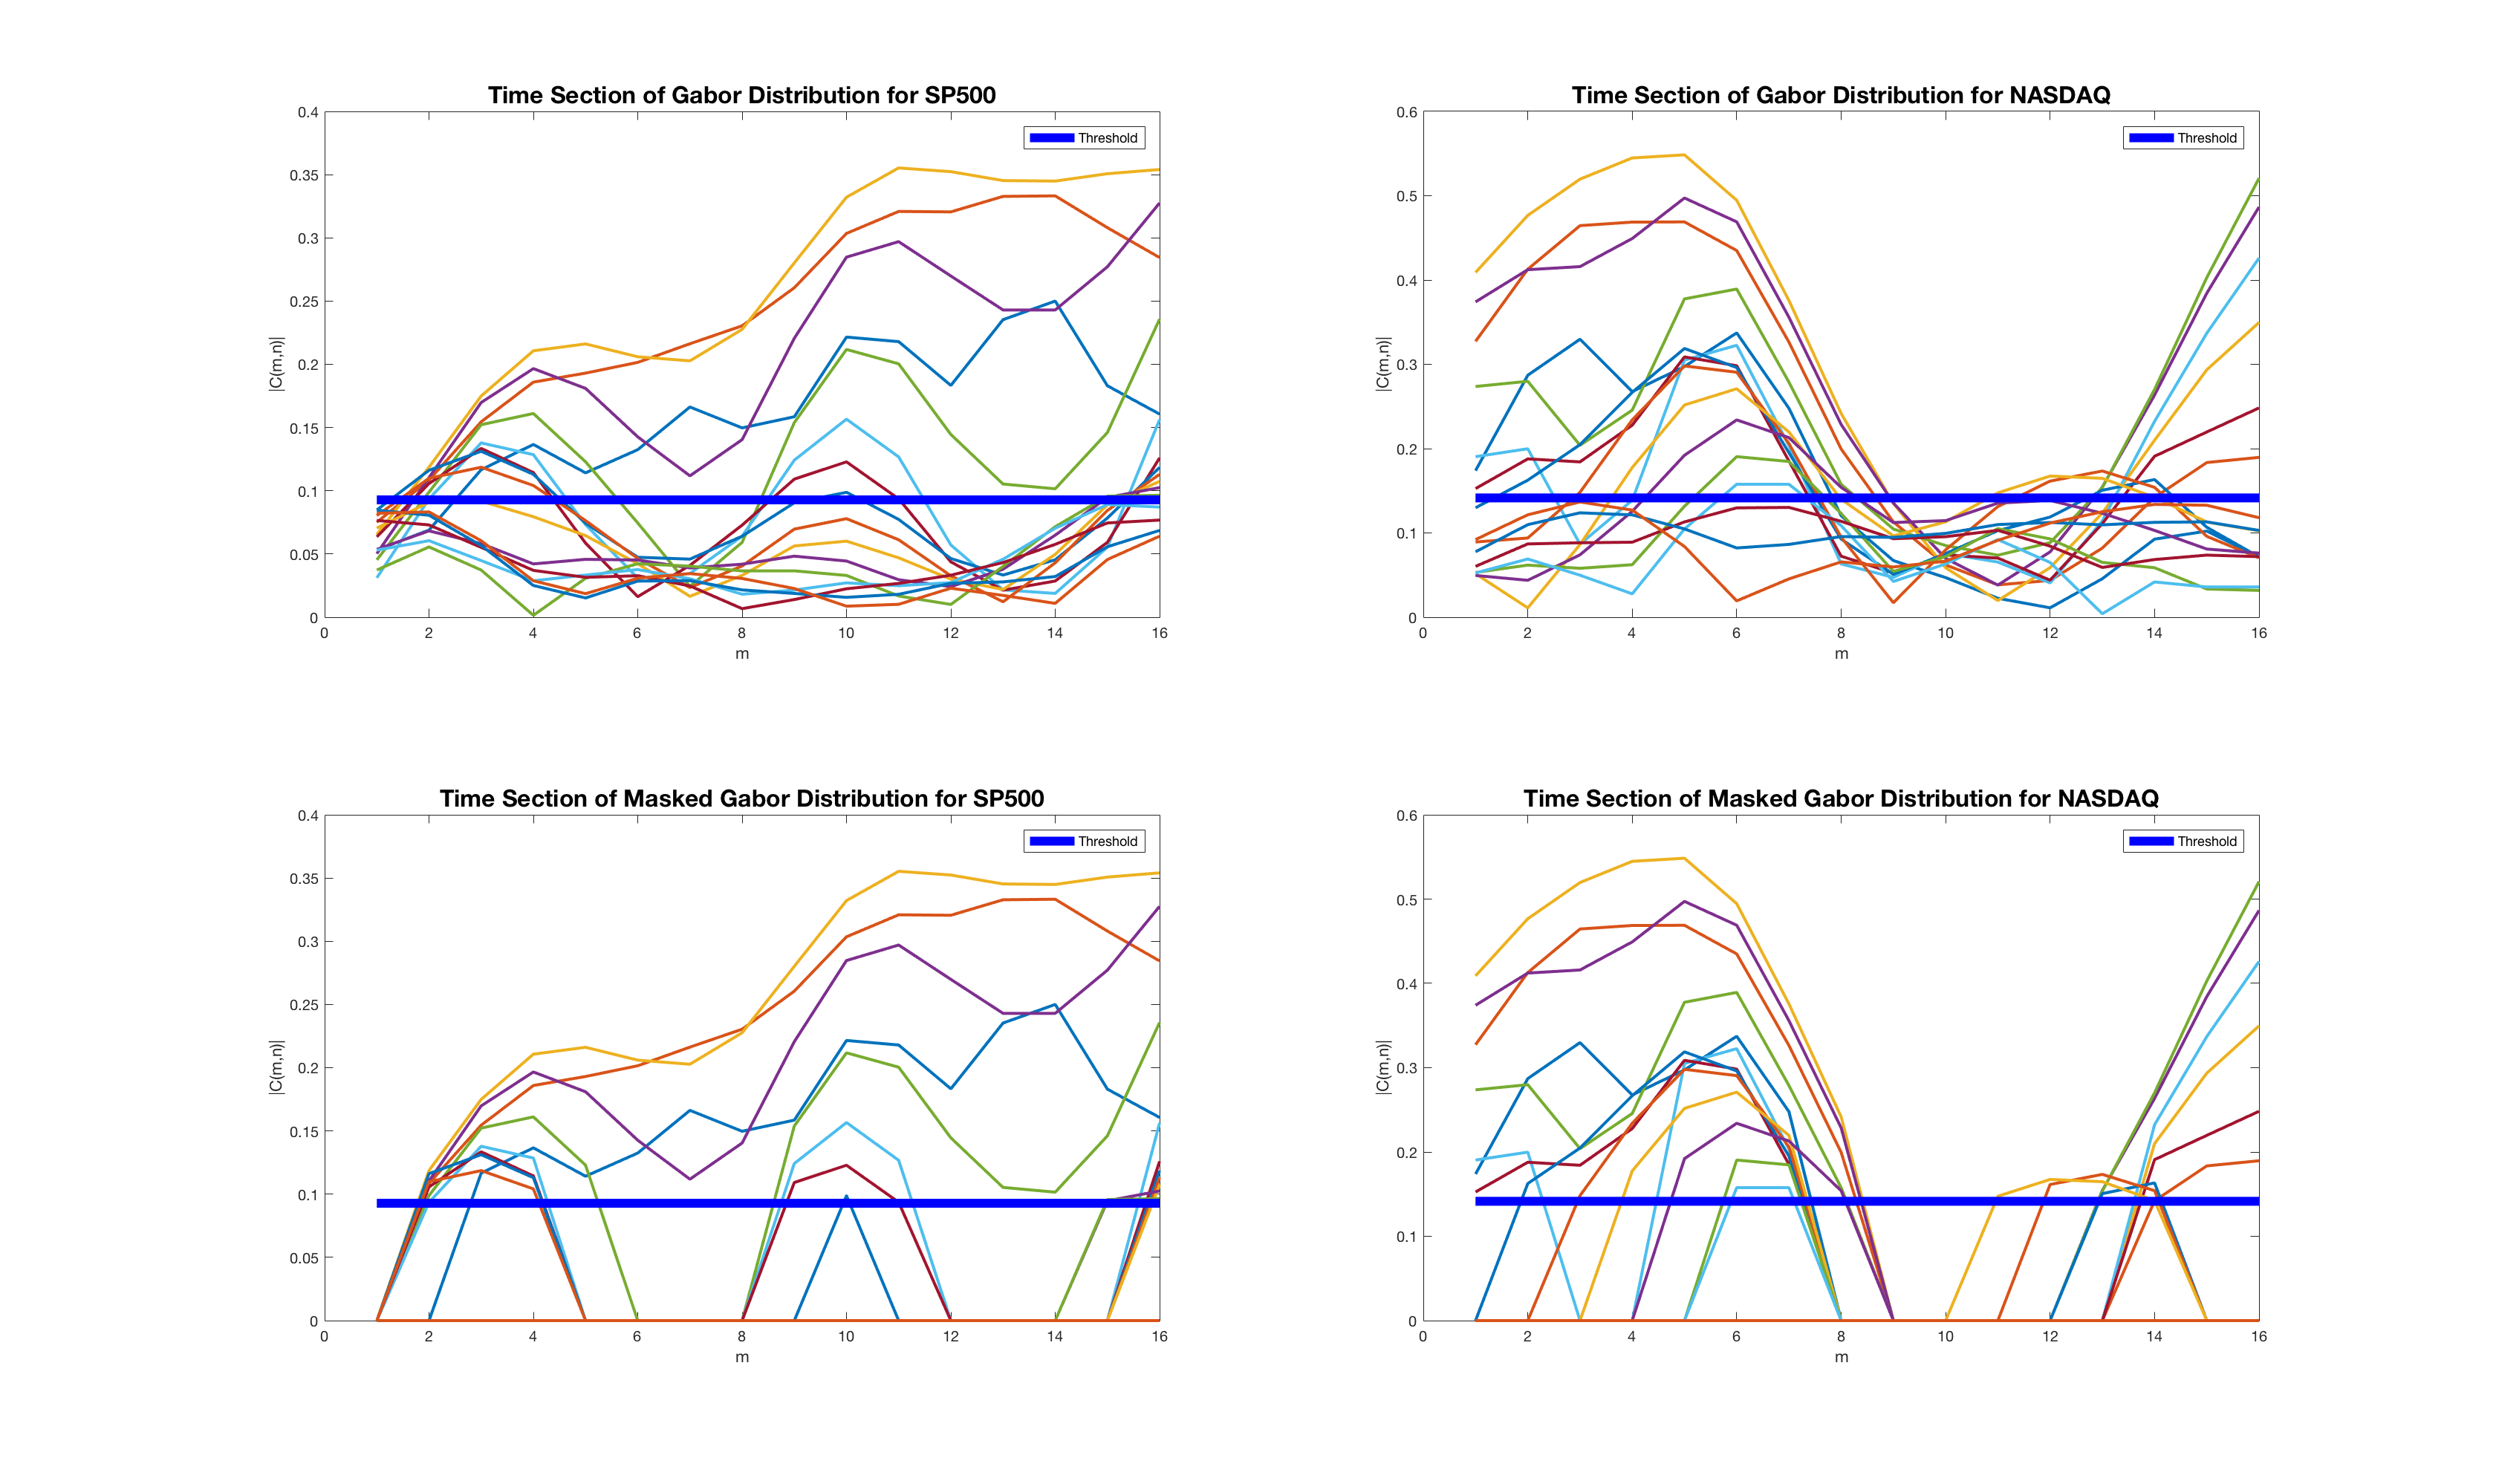
\includegraphics[scale=.15]{Images/GaborPST16}
\caption{Fig a is the time section of Gabor distribution of HP Filter cycles log(SP500) and Fig b is the time section of Gabor distribution of for HP Filter cycles log(NASDAQ). $\Delta M = 8; \Delta N = 4; m = 16; n = 32; \sigma = \sqrt{\frac{\Delta M L}{\Delta N 2\pi}}$. Threshold is calculated as $max(|c(m,n)|-min(|c(m,n)|))/2$. Mask operator used to eliminate values below threshold. The program used to create the graph is mygaborfilt.m and it is attached in the appendix.}
\label{fig:GaborPST16}
\end{figure}


\begin{figure}[!ht]
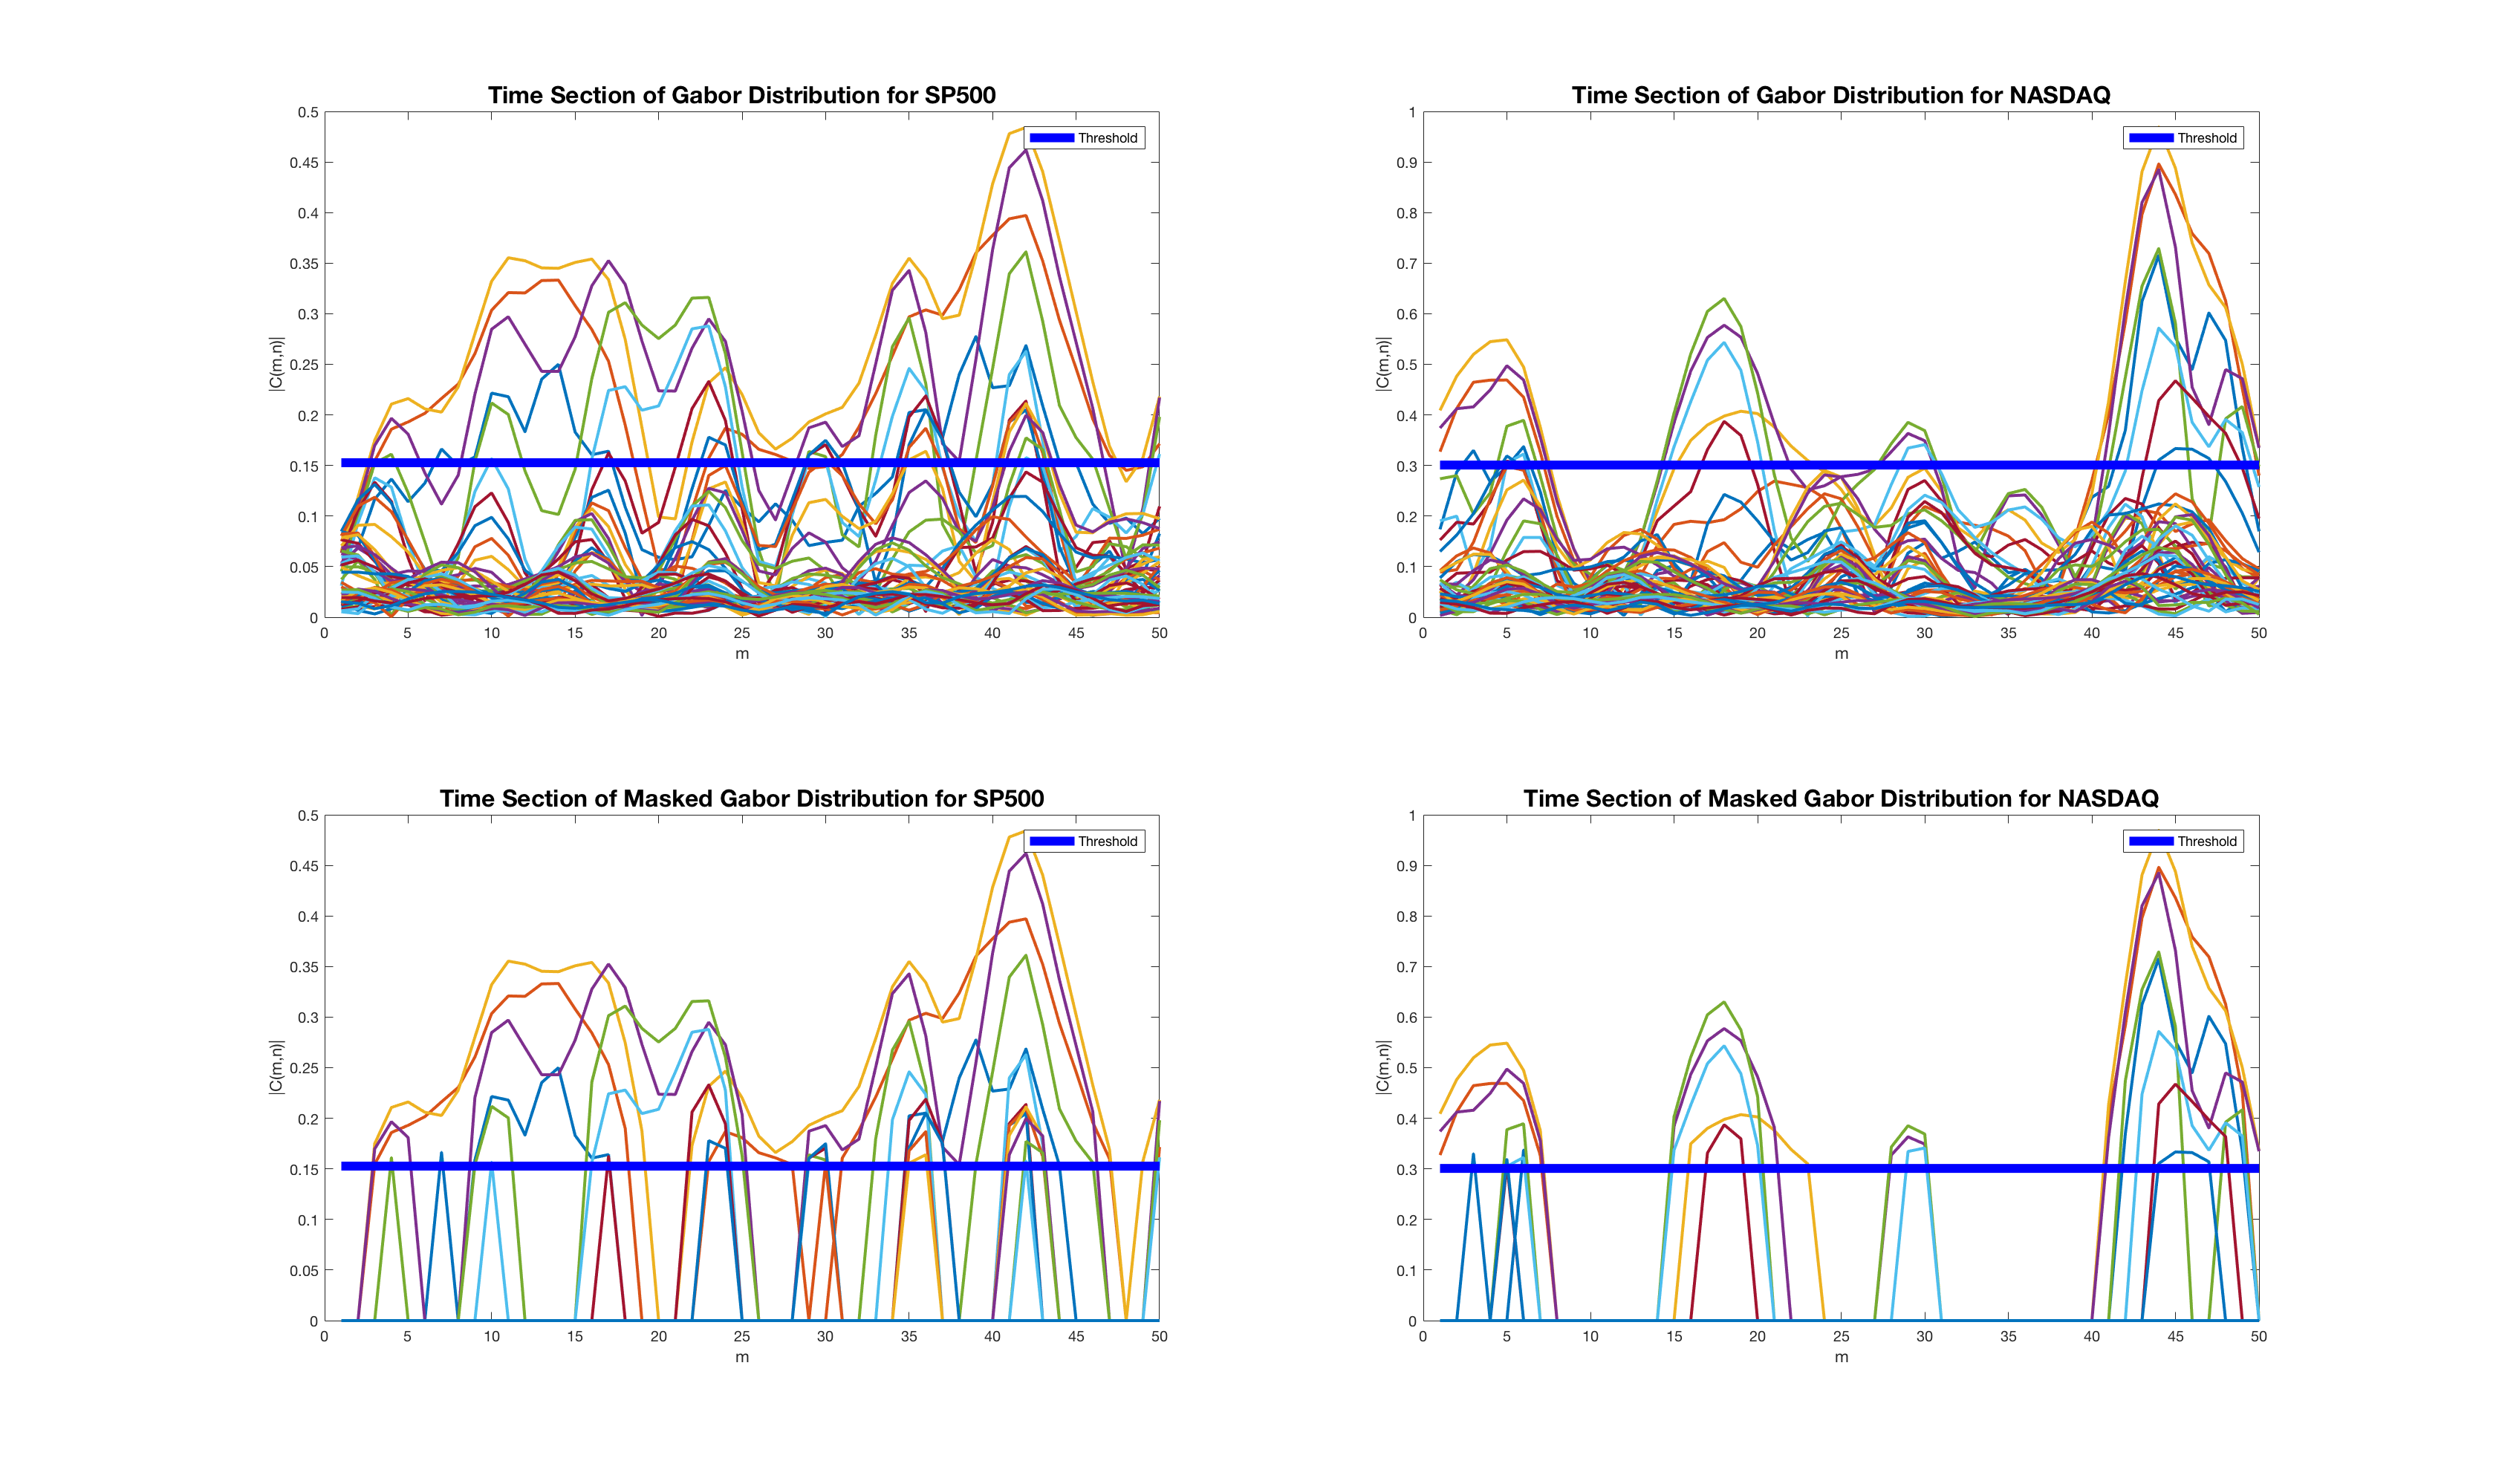
\includegraphics[scale=.15]{Images/GaborPST50}
\caption{Fig a is the time section of Gabor distribution of HP Filter cycles log(SP500) and Fig b is the time section of Gabor distribution of for HP Filter cycles log(NASDAQ). $\Delta M = 8; \Delta N = 4; m = 50; n = 100; \sigma = \sqrt{\frac{\Delta M L}{\Delta N 2\pi}}$. Threshold is calculated as $max(|c(m,n)|-min(|c(m,n)|))/2$. Mask operator used to eliminate values below threshold. The program used to create the graph is mygaborfilt.m and it is attached in the appendix.}
\label{fig:GaborPST50}
\end{figure}



\begin{equation*}
\Delta t\Delta f = \sqrt{\frac{\int_{-\infty}^{\infty}{\psi(t)(\mu_t - t)^2\psi ^*(t)dt}}{\int_{-\infty}^{\infty}{\psi(t)\psi ^*(t)dt}} \frac{\int_{-\infty}^{\infty}{\Psi(f)(\mu_f - f)^2\Psi ^*(f)df}}{\int_{-\infty}^{\infty}{\Psi(f)\Psi ^*(f)df}}} \geq \frac{1}{4\pi}
\end{equation*}


There are three possibilities for the above equation given below in table ~\ref{table:sampling} .

\begin{table}[h!]
\centering
\begin{tabular}{|c|c|c|ccc|}
  \hline
  % after \\: \hline or \cline{col1-col2} \cline{col3-col4} ...
  \textbf{$\Delta t$  $\Delta f$} & \textbf Sampling & Remarks \\
  \hline
  = $\frac{1}{4\pi}$ & Critical   & Special functions called GEF \\
  \hline
   $>$ $\frac{1}{4\pi}$ & Over   & -- \\
  \hline
  $<$ $\frac{1}{4\pi}$ & Under   & This case is not possible \\
  \hline
\end{tabular}
\caption{Possible values for $\Delta$t $\Delta$f and special case for Gabor function}
\label{table:sampling}
\end{table}

Analogous to 1D uncertainty principle, there are two 2D uncertainty principles constraining the effective width ($\Delta x$) and the effective length ($\Delta y$) of a signal $f(x,y)$ and the effective width ($\Delta u$) and the effective length ($\Delta v$) of its 2D Fourier transform $F(u,v)$. 2D Gabor transformation has wide application in image processing domain and the 2D analysis is out of scope for this project.  


\begin{equation*}
\Delta x\Delta u = \sqrt{\frac{\int_{-\infty}^{\infty}{\psi(x,y)(\mu_x - x)^2\psi ^*(x,y)dxdy}}{\int_{-\infty}^{\infty}{\psi(x,y)\psi ^*(x,y)dxdy}} \frac{\int_{-\infty}^{\infty}{\Psi(u,v)(\mu_u - u)^2\Psi ^*(u,v)dudv}}{\int_{-\infty}^{\infty}{\Psi(u,v)\Psi ^*(u,v)dudv}}} \geq \frac{1}{4\pi}
\end{equation*}


\begin{equation*}
\Delta y\Delta v = \sqrt{\frac{\int_{-\infty}^{\infty}{\psi(x,y)(\mu_y - y)^2\psi ^*(x,y)dxdy}}{\int_{-\infty}^{\infty}{\psi(x,y)\psi ^*(x,y)dxdy}} \frac{\int_{-\infty}^{\infty}{\Psi(u,v)(\mu_v - v)^2\Psi ^*(u,v)dudv}}{\int_{-\infty}^{\infty}{\Psi(u,v)\Psi ^*(u,v)dudv}}} \geq \frac{1}{4\pi}
\end{equation*}

\begin{equation*}
\Delta x\Delta u  \Delta y\Delta v    \geq \frac{1}{16\pi^2}
\end{equation*}


\chapter{Wigner Distribution}
 \label{chap:Wigner}
 \input{Chap3/chap3}

\chapter{Time Frequency Distribution Series}
 \label{chap:TFDS}
 \section{Time Frequency Distribution Series}

The main drawback of the Wigner Ville distribution is cross term interference and the cross term oscillates and is localized. 

Time Frequency Distribution Series (TFDS) was introduced by Chen and Qian \cite{pchen} as the decomposition of the Wigner Ville distribution via the orthogonal like Gabor expansion. Let me walk through each step to attain the time frequency distribution series. 

Let $g(t)$ be a normalized Gaussian function which is defined as follows. 

\begin{equation}
g(t) = \frac{1}{{(\pi \sigma^2)}^{0.25}} e^{-\frac{t^2}{2 \sigma^2}}
\end{equation}

The corresponding Wigner Ville Distribution (WVD) is given below.

\begin{equation}
WVD_g(t,\omega) = 2 e^{-(\frac{t^2}{\sigma^2}+\sigma^2\omega^2)}
\end{equation}

The $WVD_g(t,\omega)$ is centered at origin and it decays exponentially in both the time and frequency domains. The contour plot of the $WVD_g(t,\omega)$ consists of concentric ellipses and it is given below.


\begin{figure}[!ht]
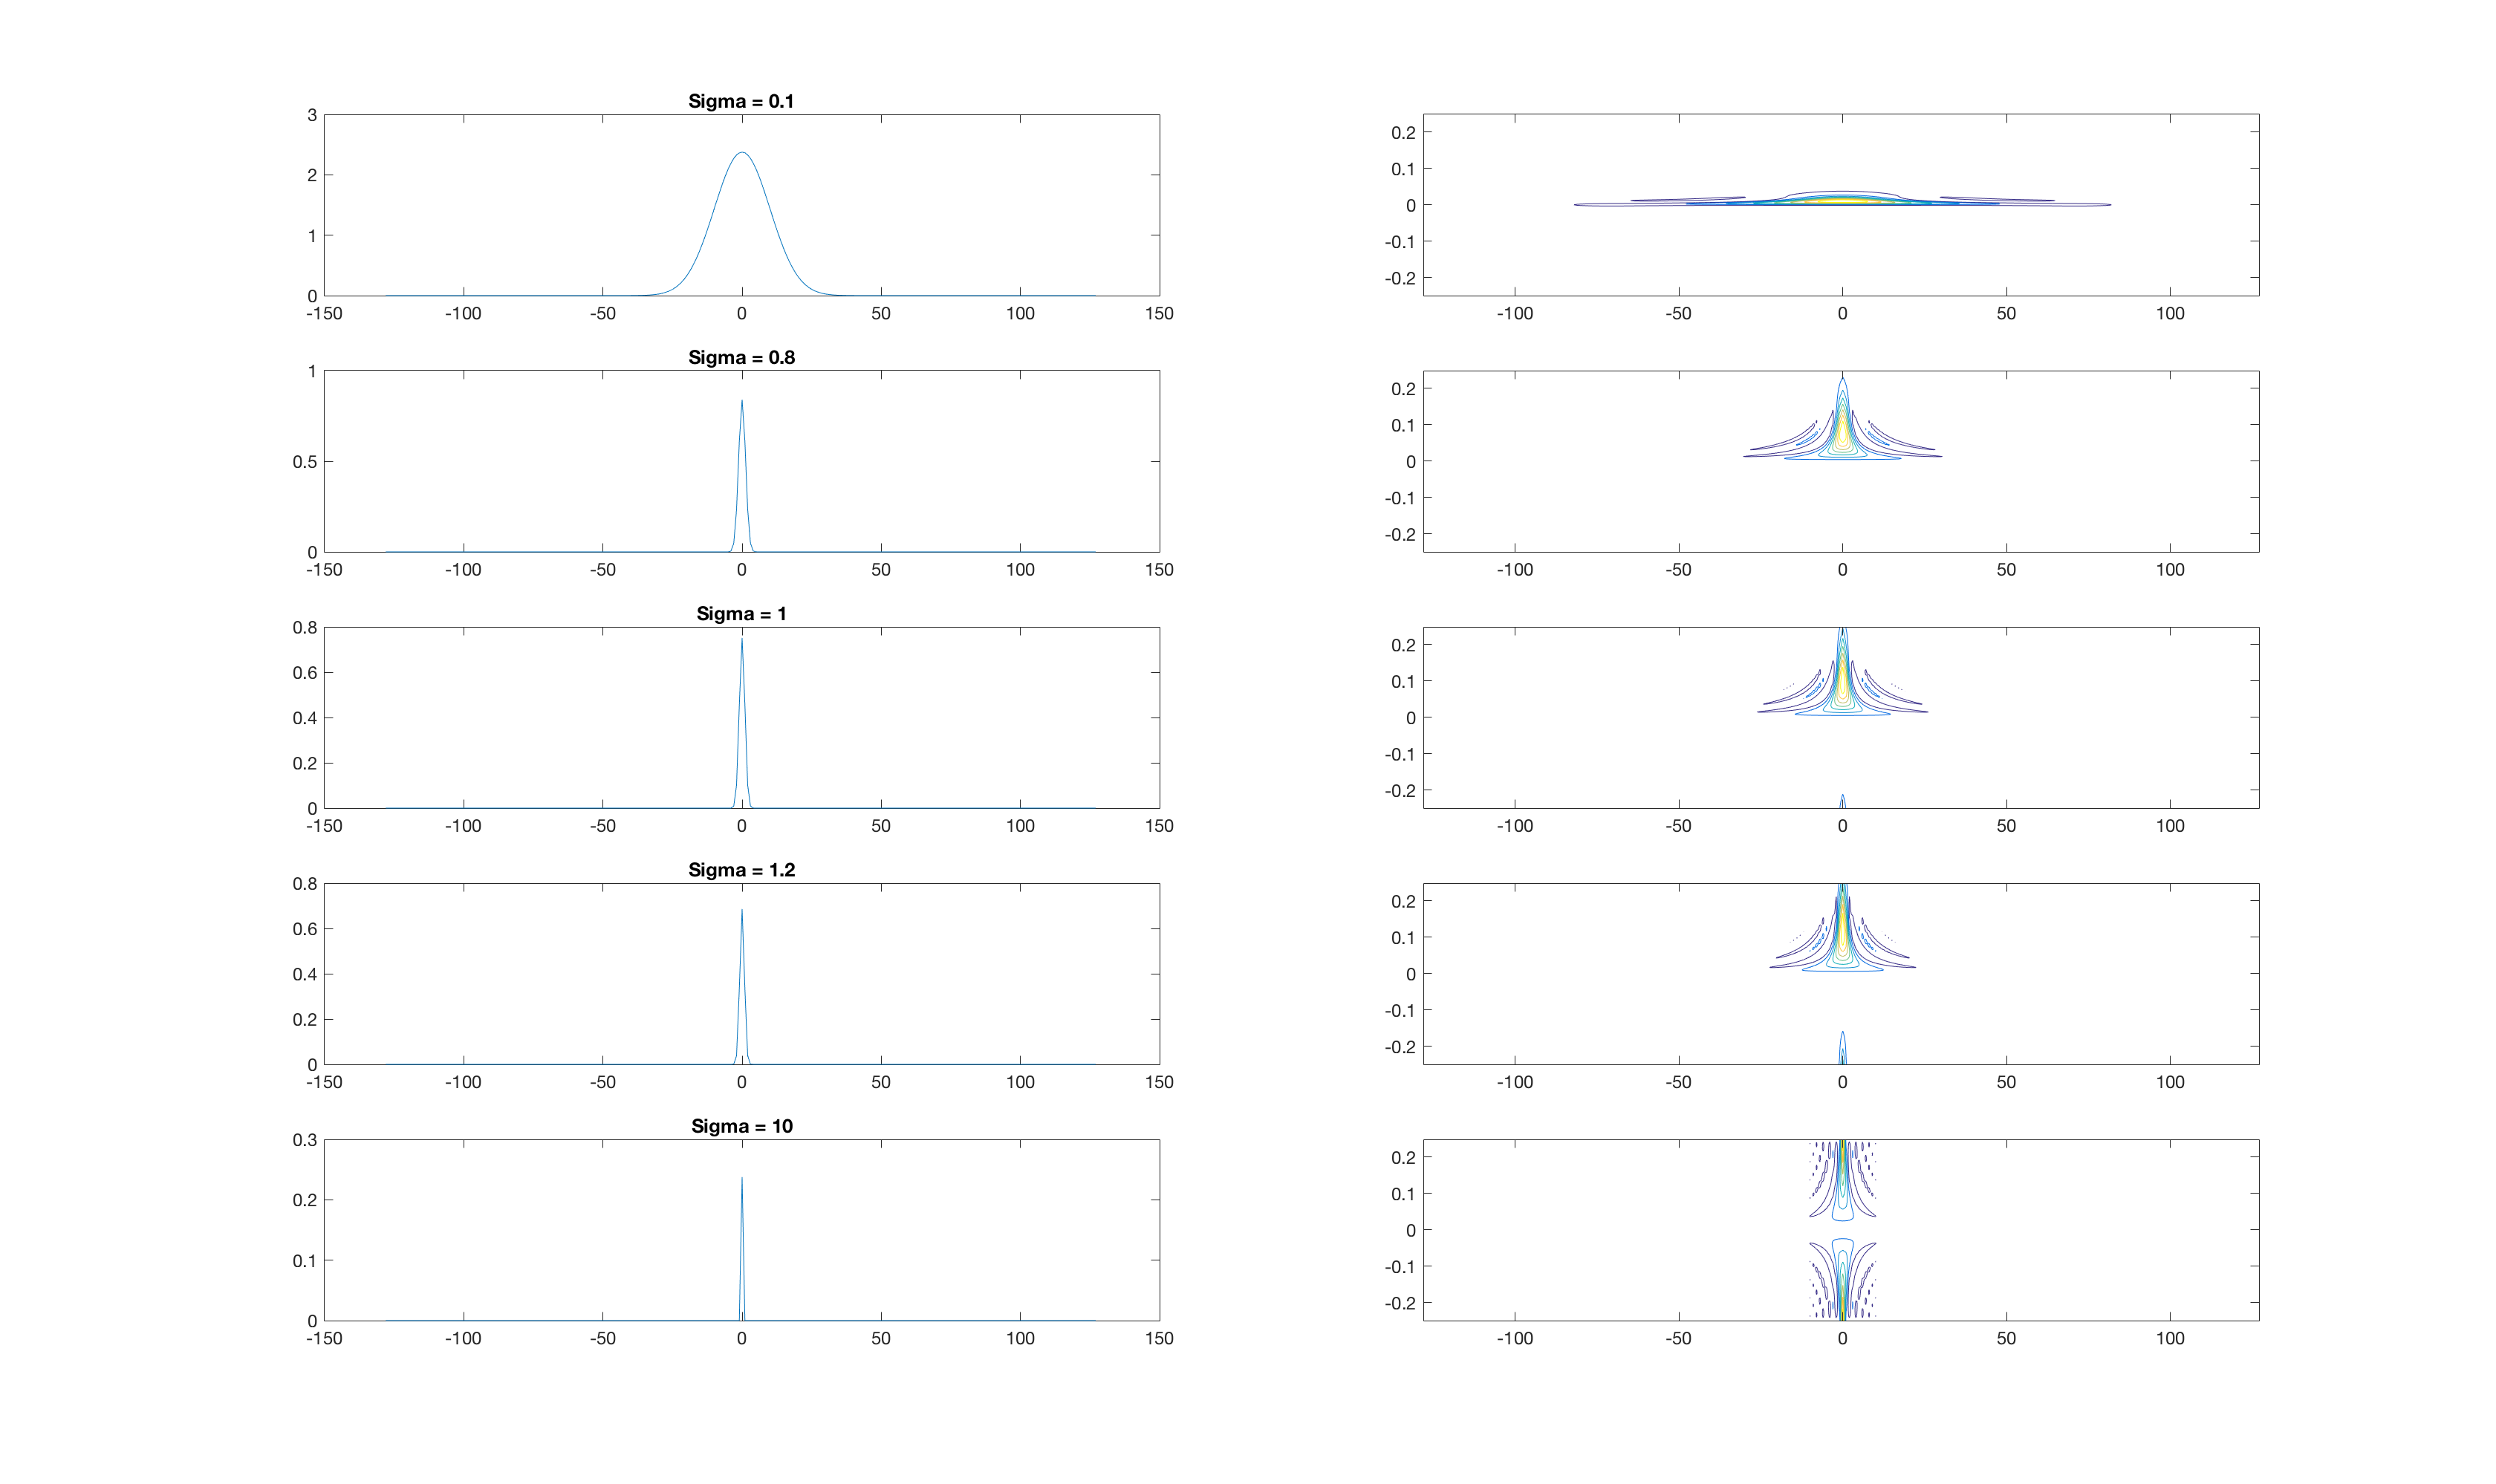
\includegraphics[scale=.15]{Images/WVD_gauss}
\caption{Fig in the left hand side represents the Gaussian function $g(t)$ as defined above for various $\sigma$ values. Fig in the right land side represents the Wigner Ville Distribution $WVD_g$ as defined above. The graph is created using the mywvdgauss.m program attached in the Appendix. $WVD$ values are created by using the HOSA (Higher Order Spectral Analysis) Matlab toolbox. }
\label{fig:WVD_gauss}
\end{figure}

The WVD is time and frequency-shift invariant. Let

\begin{equation}
h(t) = g(t-mT) e^{-jn\Omega t}
\end{equation} where $\Omega$ and $T$ are the frequency and time sampling steps respectively. The WVD of $h(t)$ is given by,

\begin{equation}
WVD_h(t,\omega) = 2e^{-[\frac{(t-mT)^2}{\sigma^2}+[\sigma(\omega-n\Omega)]^2]}
\end{equation}

\begin{equation}
WVD_h(t,\omega) = WVD_g(t-mT,\omega-n\Omega)
\end{equation}

Let $s(t) = h(t)+h'(t)$, then $WVD_s(t,\omega)$ is given as
\begin{equation}
WVD_s(t,\omega) = WVD_h(t,\omega)+WVD_{h'}(t,\omega)+2Re[{WVD_{h,h'}(t,\omega)}]
\end{equation}

where $WVD_{h,h'}(t,\omega)$ is given by
\begin{equation}
 WVD_{h,h'}(t,\omega) = e^{j\omega_d t_\mu} H(t-t_\mu, \omega-\omega_\mu)
\end{equation}

where
\begin{equation}
H(t,\omega) = 2e^{-[\frac{t^2}{\sigma^2}+(\sigma \omega)^2]} e^{-j[t_d\omega - \omega_dt]}
\end{equation}

\begin{equation}
\begin{aligned}
t_\mu &= \frac{m+m'}{2} T  \\
\omega_\mu &= \frac{n+n'}{2}\Omega \\
t_d &= (m - m')T \\
\omega_d &= (n-n')\Omega 
\end{aligned}
\end{equation}

The $WVD_{h,h'}(t,\omega)$ has the same envelope as the $WVD_g(t,\omega)$ but is oscillating with frequency $\omega_d$ in the time domain and $t_d$ in the frequency domain. The location of $WVD_{h,h'}(t-t_\mu,\omega-\omega_\mu)$ is halfway between $h$ and $h'$. The $2Re$[$WVD_{h,h'}(t,\omega)$] is the cross term. When a signal $s(t)$ can be decomposed as a linear combination of some elementary functions $h(t)$ then the cross-terms can be controlled. 

Recall from the previous chapter on the Gabor Expansion, for a given signal $s(t)$, the orthogonal-like Gabor expansion is defined as follows. 

\begin{equation}
s(t) = \frac{1}{\sqrt{2\pi}} \sum_{m=-\infty}^{\infty} \sum_{n=-\infty}^{\infty} C_{m,n} g(t-mT) e^{jn\Omega t}
\end{equation}

The Gabor coefficients $C_{m,n}$ are determined by

\begin{equation}
C_{m,n} = \int s(t) \gamma^{*}_{m,n}(t) dt = \int s(t) \gamma^{*}(t-mT)e^{-jn\Omega t} dt = STFT(mT,n\Omega)
\end{equation}

Using the Wigner-Ville distribution of $s(t)$ from the above equation yields,

\begin{equation}
WVD_s(t,\omega) = \sum_{m,n} \sum_{m',n'} C_{m,n} C_{m',n'} WVD_{h,h'}(t,\omega)
\end{equation}

where


\begin{equation}
 WVD_{h,h'}(t,\omega) = e^{j\omega_d t_\mu} 2e^{-[\frac{(t-t_mu)^2}{\sigma^2}+(\sigma (\omega-\omega_\mu))^2]} e^{-j[t_d\omega - \omega_d t]}
\end{equation}

\begin{equation}
WVD_s(t,\omega) = \sum_{m,n} \sum_{m',n'} C_{m,n} C_{m',n'} e^{j\omega_d t_\mu} 2e^{-[\frac{t^2}{\sigma^2}+(\sigma \omega)^2]} e^{-j[t_d\omega - \omega_dt]}
\end{equation}

where $t_d$ and $\omega_d$ reflect the degree of oscillation. 

When $m=m'$ and $n=n'$, 
\begin{equation}
C_{m,n} C^*_{m',n'} WVD_{h,h'}(t,\omega) = 2|C_{m,n}|^2 e^{-[\frac{(t-mT)^2}{\sigma^2}+\sigma^2 (\omega-n\Omega)^2)]} 
\end{equation}

When $m\neq m'$ or $n \neq n'$

\begin{equation}
C_{m,n} C^*_{m',n'} WVD_{h,h'}(t,\omega) = C_{m,n}C^{*}_{m',n'} e^{j\omega_d t_\mu} H(t-t_\mu,\omega-\omega_\mu)
\end{equation}

Based on the decomposition of the Wigner-Ville distribution defined above, the Time Frequency Distribution Series (TFDS) is defined as follows. 

\begin{equation}
TFDS_D(t,\omega) = \sum_{d=0}^{D} P_d(t,\omega)
\end{equation}

Here $P_d(t,\omega)$ is the sum of a sequence of $WVD_{h,h'}(t,\omega)$ which have a similar contribution to the useful properties and similar influence to the cross terms in which $|m-m'|+|n-n'|=d$

\begin{equation}
P_d(t,\omega) = \sum_{|m-m'|+|n-n'|=d} C_{m,n}C^{*}_{m',n'} WVD_{h,h'}(t,\omega)
\end{equation}

Substituting the value of $WVD_{h,h'}(t,\omega)$ in the above equation, we get

\begin{equation}
P_d(t,\omega) = \sum_{|m-m'|+|n-n'|=d} C_{m,n}C^{*}_{m',n'} e^{j\omega_d t_\mu} 2e^{-[\frac{t^2}{\sigma^2}+(\sigma \omega)^2]} e^{-j[t_d\omega - \omega_d t]}
\end{equation}

Substituting the value of $t_d$, $\omega_d$, $t_\mu$ and $\omega_\mu$, we get

\begin{equation}
P_d(t,\omega) = \sum_{|m-m'|+|n-n'|=d} C_{m,n}C^{*}_{m',n'} e^{j\frac{n+n'}{2}\Omega(m-m')T} 2e^{-[\frac{t^2}{\sigma^2}+(\sigma \omega)^2]} e^{-j[(m-m')T\omega - (n-n')\Omega t]}
\end{equation}

Both the SP500 and NASDAQ indices are discrete signals used for analysis. The $P_d$ is further simplified for programming convenience. 

The discrete Time Frequency Distribution Series is defined as follows. 

\begin{equation}
DTFDS_D[i,k] = TFDS_d(t,\omega) |_{ t = i\Delta t, \omega = \frac{2\pi k}{L\Delta t}}
\end{equation}
for $-\frac{L}{2} \leq k < \frac{L}{2}$ where $\frac{1}{\Delta t}$ denotes the sampling frequency. $L$ denotes the length of the signal. The discrete time frequency distribution series can be summarized as 

\begin{equation}
 TFDS_d(i,k) = \sum_{d=0}^{D} P_d[i,k]
\end{equation}

where 
\begin{equation}
 P_d[i,k] = \sum_{|m-m'|+|n-n'|=d} C_{m,n}C_{m'n'} WVD_{h,h'}[i,k]
\end{equation}

The $TFDS_D[i,k]$ is the sum of all $WVD_{h,h'}[i,k]$ in which the distance of the corresponding Gabor elementary functions $h_{m,n}[i]$ and $h_{m',n'}[i]$ is less than or equal to d. $WVD[i,k]$ is defined as a sampled Wigner-Ville distribution. 

\begin{equation}
WVD_s[i,k] = WVD_s(t,\omega) |_{ t=i\Delta t, \omega = \frac{2\pi k}{L\Delta t}}
\end{equation}
where $\Delta t$ denotes the sampling interval. For the Gaussian functions, WVD is obtained by sampling the formula. 

\begin{equation} \label{eq:1}
WVD_{h,h'}[i,k] = 2e^{-\sigma(i-\frac{m+m'}{2}\Delta M)^2-\frac{1}{\sigma}(k-\frac{n+n'}{2}\Delta N)^2} e^{j\frac{2\pi}{L}[(m-m')\Delta M k +(n-n')\Delta Ni - \frac{n+n'}{2}\Delta N(m-m')\Delta M]}
\end{equation}

We assume $\Delta t =1$. $WVD_{h,h'}[i,k]$ in \ref{eq:1} is completely determined by the parameters of the Gabor expansion, such as $\Delta M, \Delta N, L$ and $\sigma$ which are independent of the analyzed signal. Therefore, once $\Delta M, \Delta N, L$ and $\sigma$ are determined, $WVD_{h,h'}[i,k]$ can be precomputed and saved in a table. 


 \chapter{Color Chaos Model}
 \label{chap:ColorChaos}
 \section{Color Chaos}

Chen claimed in \cite{pchen}, that correlation analysis and spectral analysis are complementary tools in the stationary time-series analysis. Based on the detail study of the paper \cite{pchen}, \textbf{Color Chaos} is defined as a time frequency representation as a nonparametric approach for generalized spectral analysis for evolutionary time series. In color chaos, the HP filter is applied for trend-cycle decomposition and time-variant filters in Gabor space for pattern recognition.  Discrete-time white chaos generalized by nonlinear difference equations is tractable analytically and from the needs of empirical analysis, the continuous-time color chaos generated by nonlinear differential equations is more capable of describing business cycles than white chaos, since fluctuations and recurrent patterns can be characterized by nonlinear oscillations with irregular amplitude and a narrow frequency band in the spectrum.  Chen claimed in \cite{pchen}, the newly decoded deterministic signals from persistent business cycles reveal new sources of market uncertainty, such as changing growth-trend and shifting business cycles. 


\subsection{Role of time scale \& reference trends in representation of business cycles}

A distinctive problem in economic analysis is how to deal with growing trends in an aggregate economic time series. Both level and rate information are important when correlations are not short during business cycles. 

\textit{Time Scale}:
Chaos theory in nonlinear dynamics emphasizes the role of history, because a nonlinear deterministic system is sensitive to its initial condition. The martingale theory of the stock market ignores the path-dependent information in the stock market. The challenges faced are:
\begin{enumerate}
\item Choosing an appropriate time sampling rate is often ignored in econometric analysis. Chaotic cycles in continuous time may look like noise if the sampling time interval is not small compared to its fundamental period of a cycle.  For example, annual economic data are not capable of revealing the frequency pattern of a business cycle. 
\item Numerically, a large time unit such as the annual time series can easily obscure a cyclic pattern in the correlation analysis of business cycles.
\end{enumerate}
\textit{Reference Trend}:
How to choose a reference trend or a proper transformation to simplify the empirical pattern of business cycles? The core problem in economic analysis is not noise-smoothing but trend-defining in economic observation and decision making. There are two criteria in choosing the proper mathematical representation. 
\begin{enumerate}
\item Mathematical reliability 
\item Empirical verifiability.
\end{enumerate}
Unlike experimental economics, macroeconomic time series are not reproducible in history. Traditional tests in econometric analysis have limited power in studies of an evolutionary economy containing deterministic components.  A good fit of past data does not guarantee the ability for better future predictions.  There are two extreme approaches in econometric analysis: the trend-stationary (TS) approach of log-linear detrending (LLD) and the difference-stationary (DS) approach of first differencing (FD).  A compromise between these two extremes is the Hodrick and Prescott (HP) filter.  In principle, a choice of observation reference is associated with a theory of economic dynamics. Log-linear detrending implies a constant exponential growth as shown in the figure ~\ref{fig:LogLinear}. 

The FD detrending produces a noisy picture that is predicted by the random-walk model with a constant drift (or the so-called unit-root model in econometric literature).  Economically speaking, the FD detrending in econometrics implies that the level information in price indicators can be ignored in economic behavior.  This assertion may conflict with many economic practices, since traders constantly watch economic trends, and no one will make an investment decision based only on the current rate of price changes.  The error-correction model in econometrics tried to remedy the problem by addition some lagged-level information, such as using a one-year-before level as an approximation of the long-run equilibrium. Then comes the problem of what is the long run equilibrium in the empirical sense.  A proper decomposition of trend and cycles may find an appropriate scheme to weigh the short-term and long-run impacts of economic movements in economic dynamics.  The essence of trend-cycle decomposition is finding an appropriate time window, or equivalently, a proper frequency window, for observing time-dependent movements.  Log-linear detrending is a low-pass filter or wave detector, while first differencing is a high-pass filter or noise amplifier. 

The main drawback of LLD detrending is its over-dependence on historical boundaries, while the DS series is too erratic from amplifying high-frequency noise. 

HP filter has two advantages. 
\begin{enumerate}
\item It is localized approach in detrending, with the problem of boundary dependence. 
\item Frequency response is in the range of business cycles. 
\end{enumerate}

\subsection{Dimensionality}

\subsection{Correlation Dimension}
The correlation dimension provides a tool to quantify self-similarity. A larger correlation dimension corresponds to a larger degree of complexity and less self-similarity. The most frequently used procedure to estimate the correlation dimension was introduced by Grassberger and Procaccia (1983). They defined the correlation sum for a collection of points $X_i$ $(i=1,2,3,..,N)$ in some phase space to be the fraction of all possible pairs of points which are closer than a given distance $\epsilon$ in a particular norm:

To compute the correlation sum $C(m,\epsilon)$ and the correlation dimension $D_c$, first delay-coordinate embed the signal as follows:


$X(t) = {x(t), x(t+\tau), x(t+2\tau),..,x(t+(m-1)\tau)}$

where $\tau$ is the delay time, and $m$ is the embedding dimension. 

\begin{equation} \label{cd:1}
C(m,\epsilon) = \frac{2}{(N-m)(N-m-1)} \sum_{i=m}^{N}\sum_{j=i+1}^{N} \Theta (\epsilon - \lVert X_i - X_j \rVert )
\end{equation}

where $\Theta$ is Heaviside step function, $\Theta(x) = 0$ if $x \le 0 $ and $\Theta(x) = 1$ for $x>0$ and $X_i = X(t_i)$.
Thus equation \ref{cd:1} counts the pairs $(X_i,X_j)$ whose distance is smaller than $\epsilon$.  When ${N\to\infty}$, for small values of $\epsilon$, C follows a power law;

\begin{equation} \label{cd:2}
C(\epsilon) \propto \epsilon^{D_c}
\end{equation}

where $D_c$ is correlation dimension. Therefore, $D_c$ is defined as
\begin{equation} \label{cd:3}
D_c = \lim_{\epsilon\to 0} \lim_{N\to\infty} \frac{\partial log_{10} C(\epsilon)}{\partial log_{10}(\epsilon)}
\end{equation}

Correlation dimension is estimated by computing the slope of the straight line by using least square fit in a plot of $log_{10} C(\epsilon)$ vs $log_{10}(\epsilon)$.

\begin{figure}[!ht]
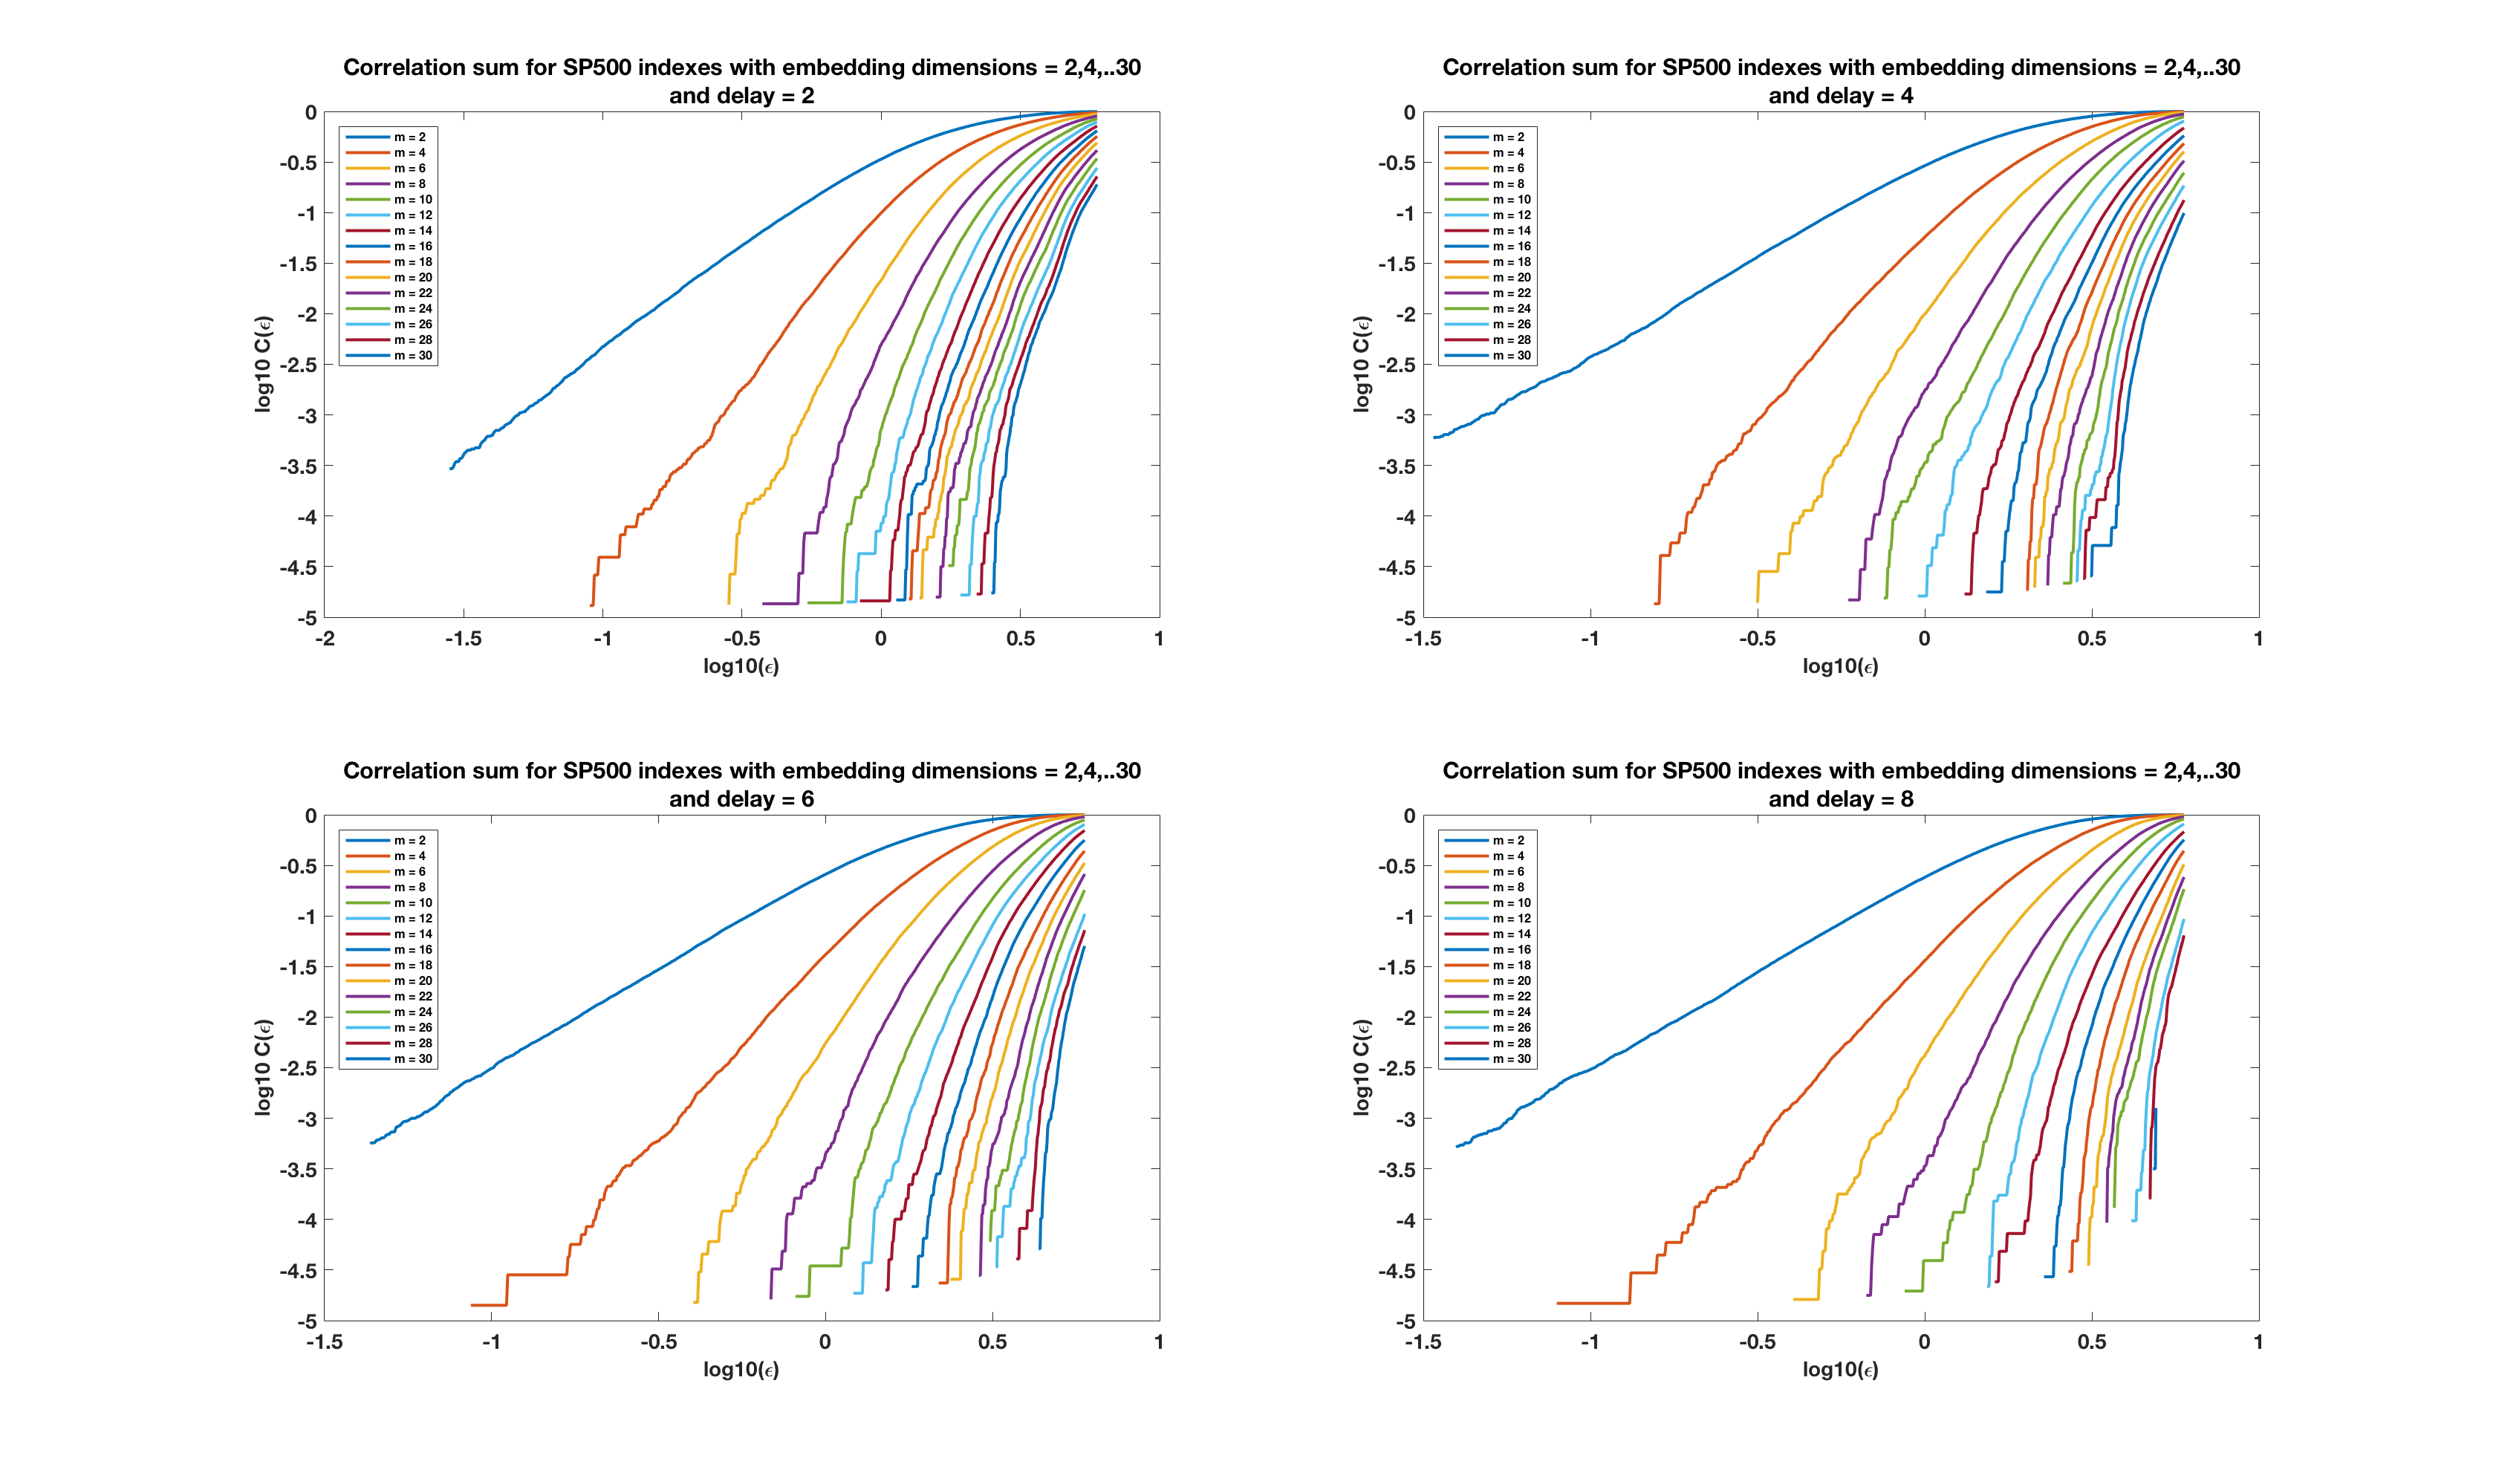
\includegraphics[scale=.15]{Images/SP500CD1}
\caption{Correlation Dimension for NASDAQ. The graph was created by using drawCorrDim.m and it is attached in the Appendix}
\label{fig:SP500CD1}
\end{figure}

\begin{figure}[!ht]
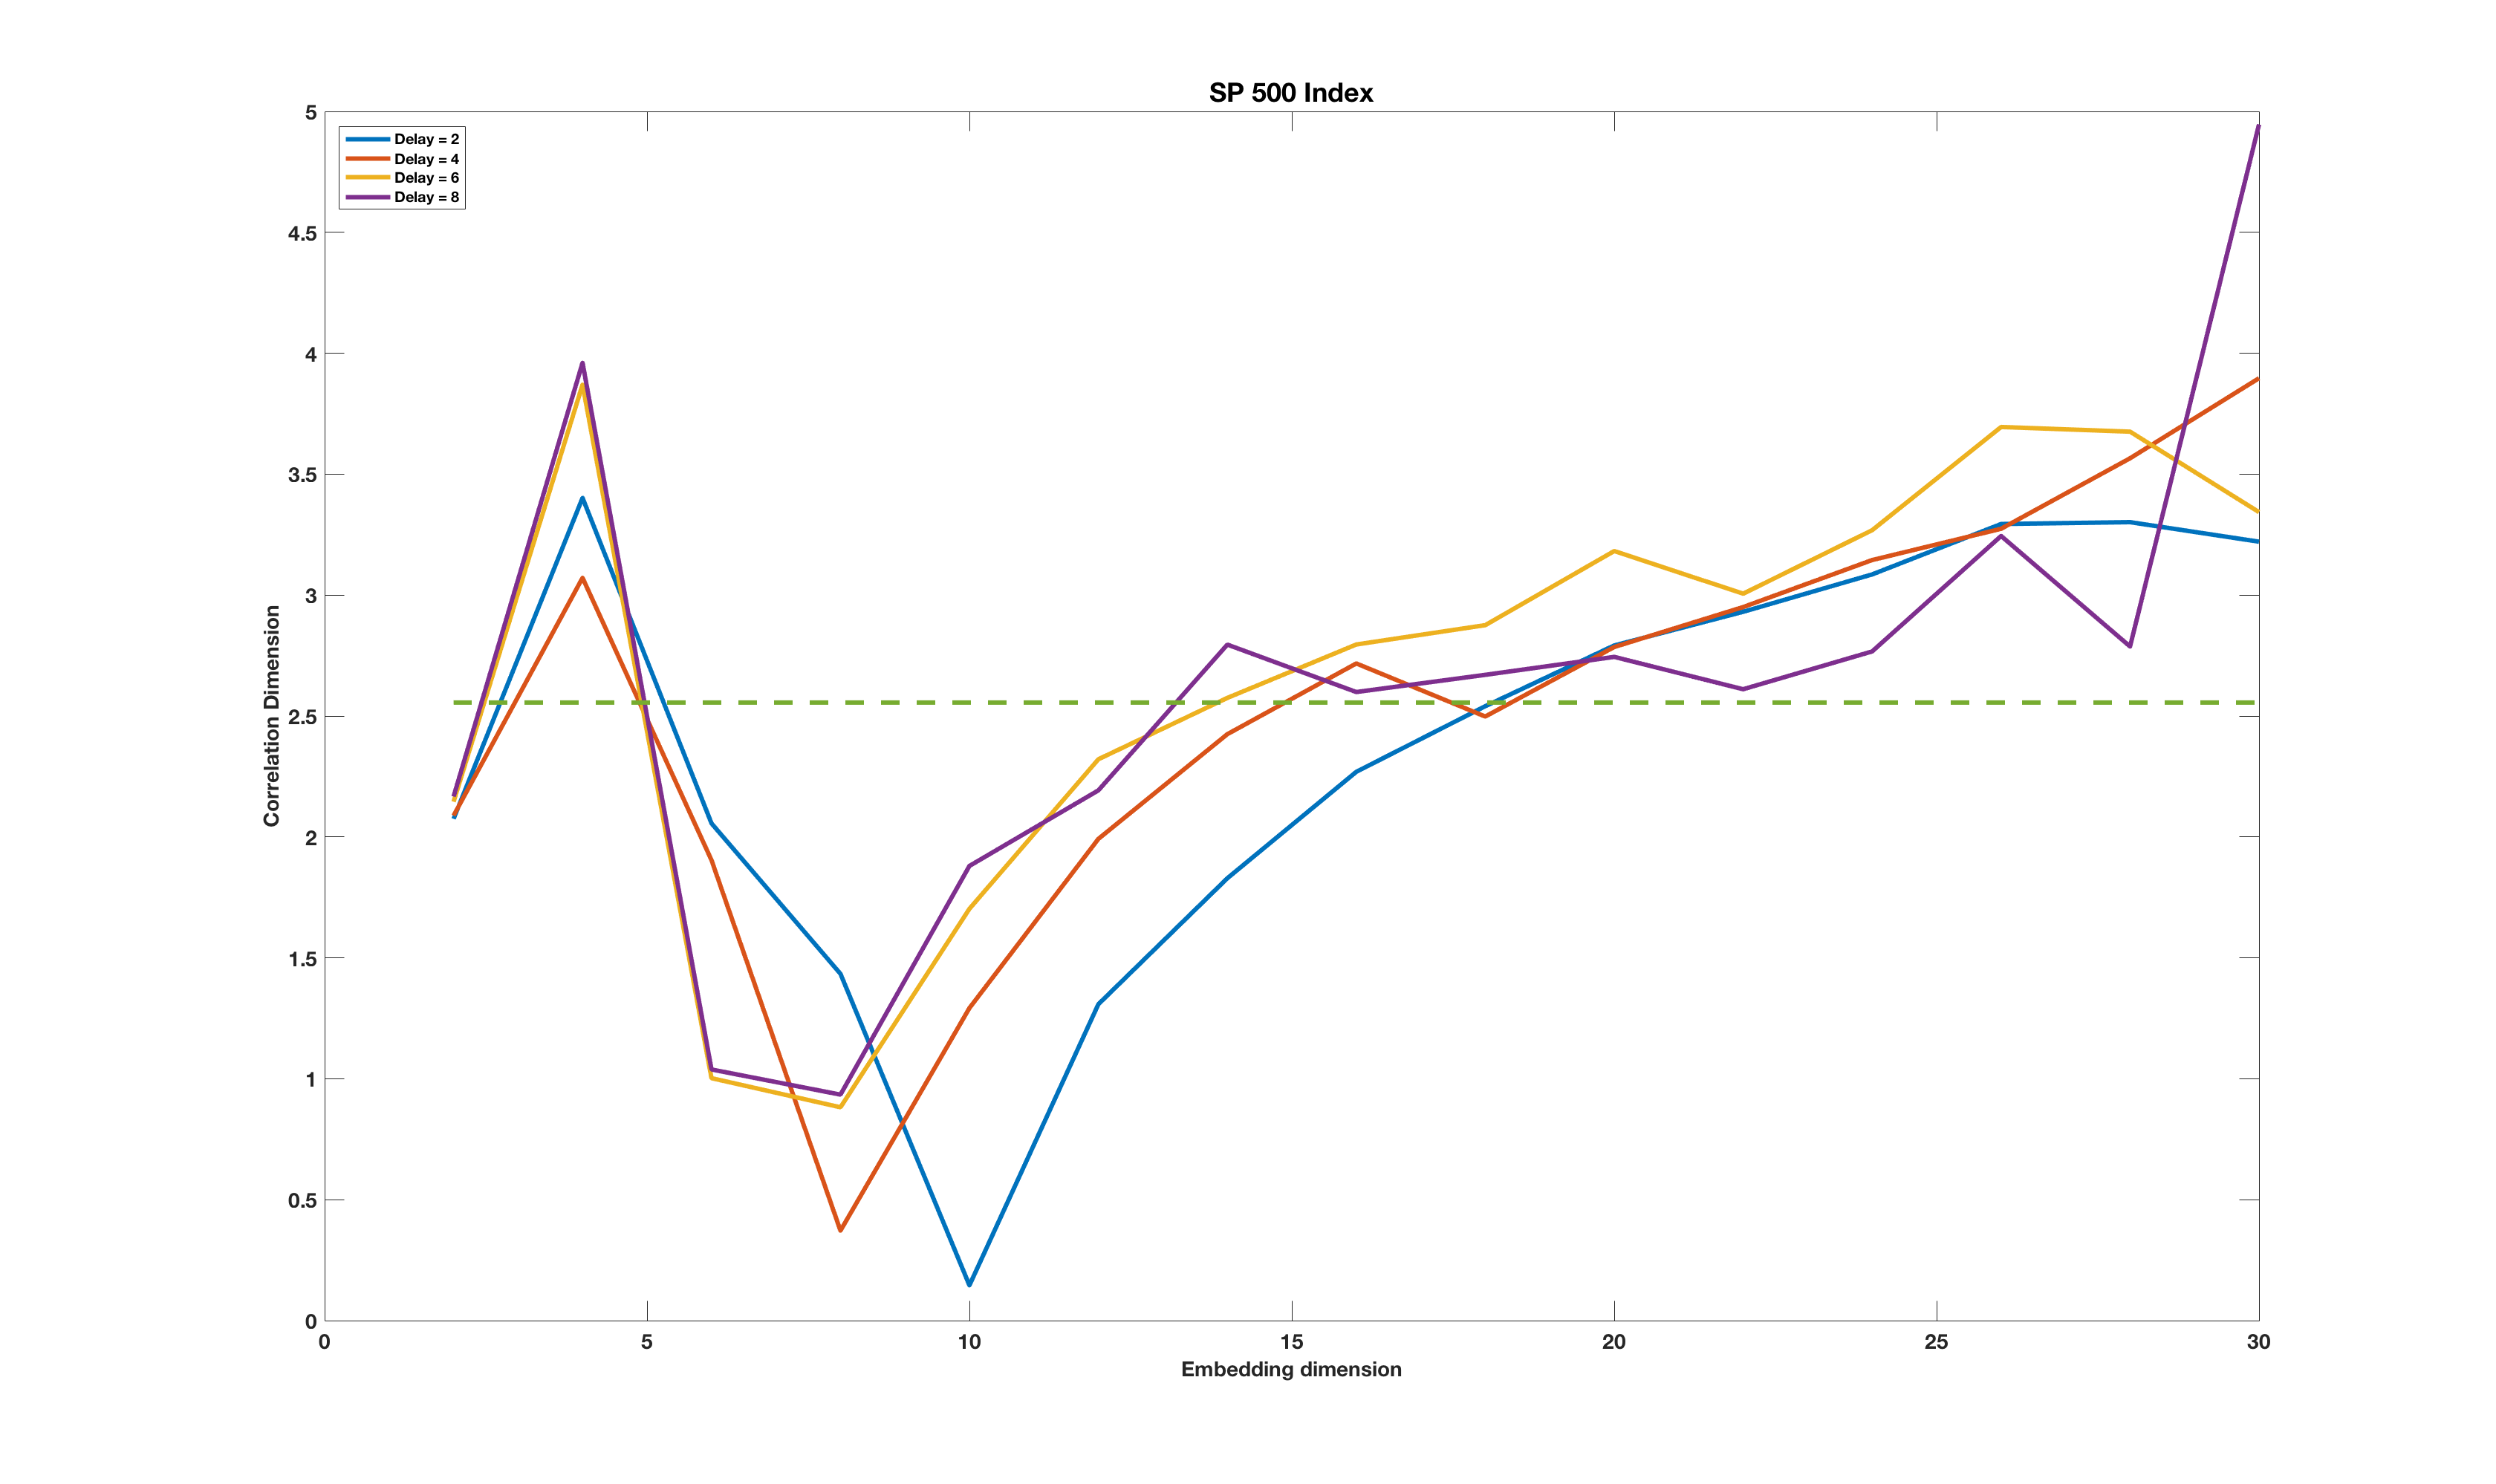
\includegraphics[scale=.15]{Images/SP500CD2}
\caption{Correlation Dimension for NASDAQ. The graph was created by using drawCorrDim.m and it is attached in the Appendix}
\label{fig:SP500CD2}
\end{figure}

\begin{figure}[!ht]
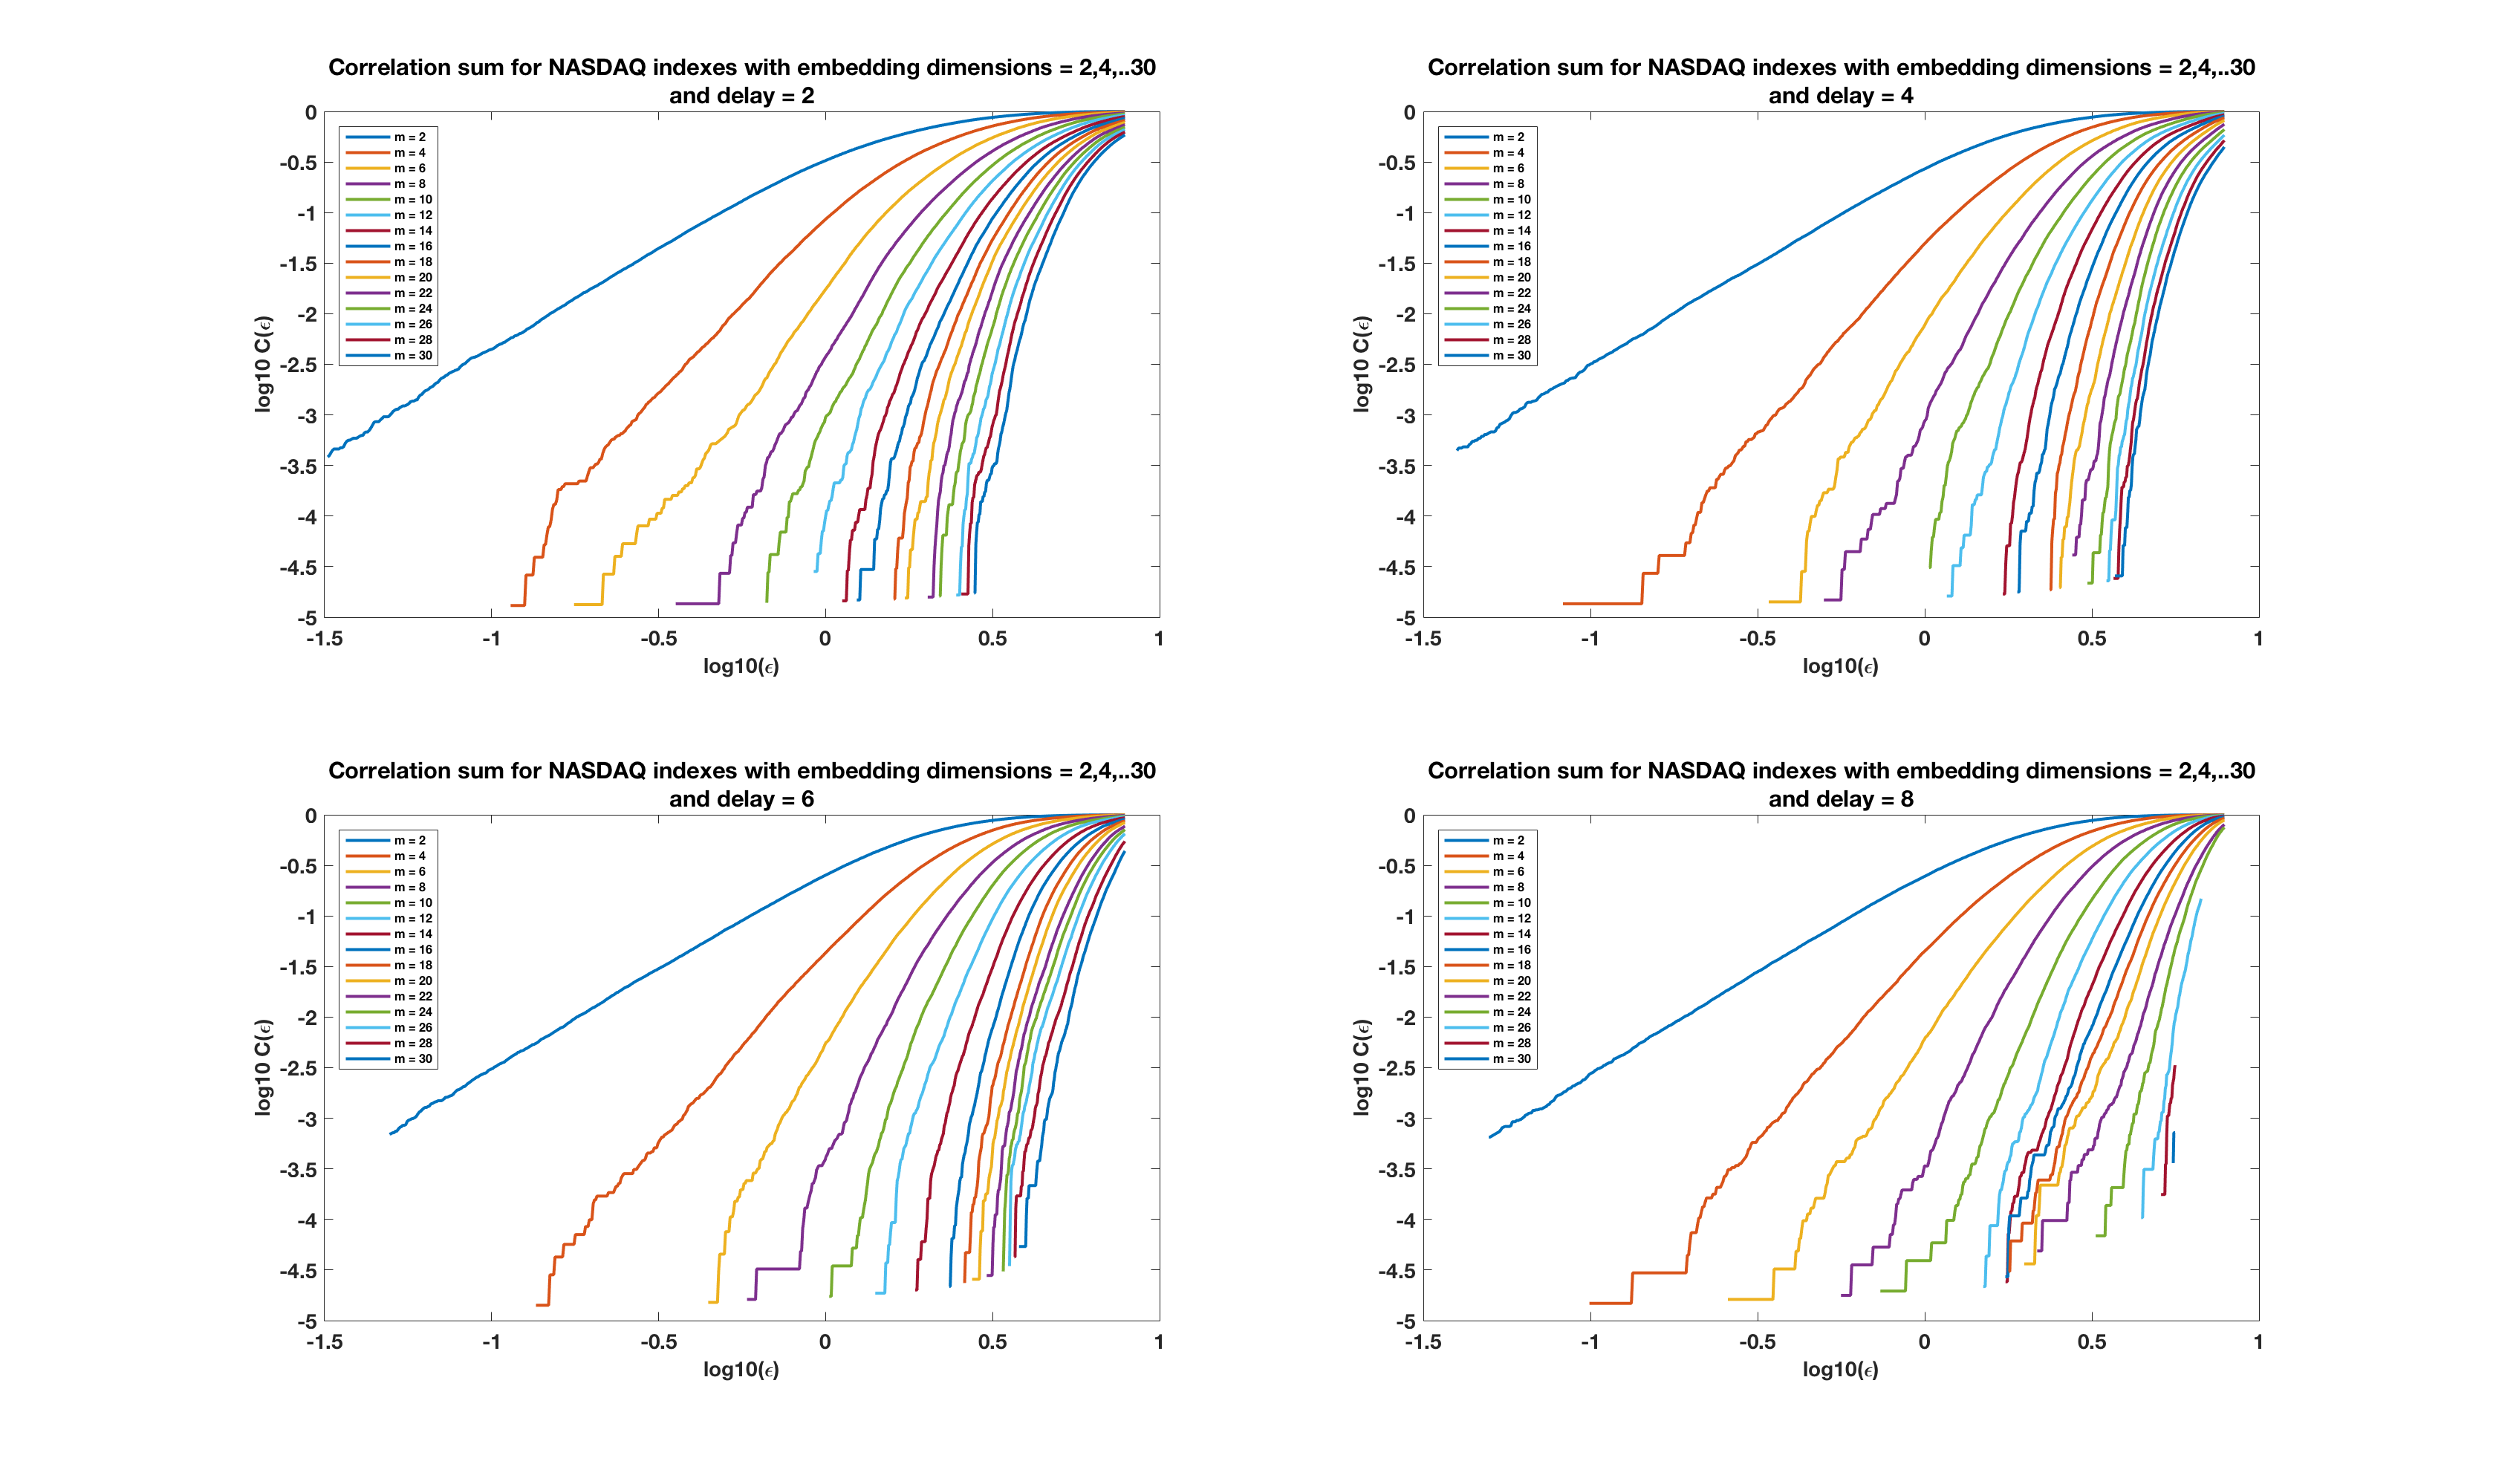
\includegraphics[scale=.15]{Images/NASDAQCD1}
\caption{Correlation Dimension for NASDAQ. The graph was created by using drawCorrDim.m and it is attached in the Appendix}
\label{fig:NASDAQCD1}
\end{figure}

\begin{figure}[!ht]
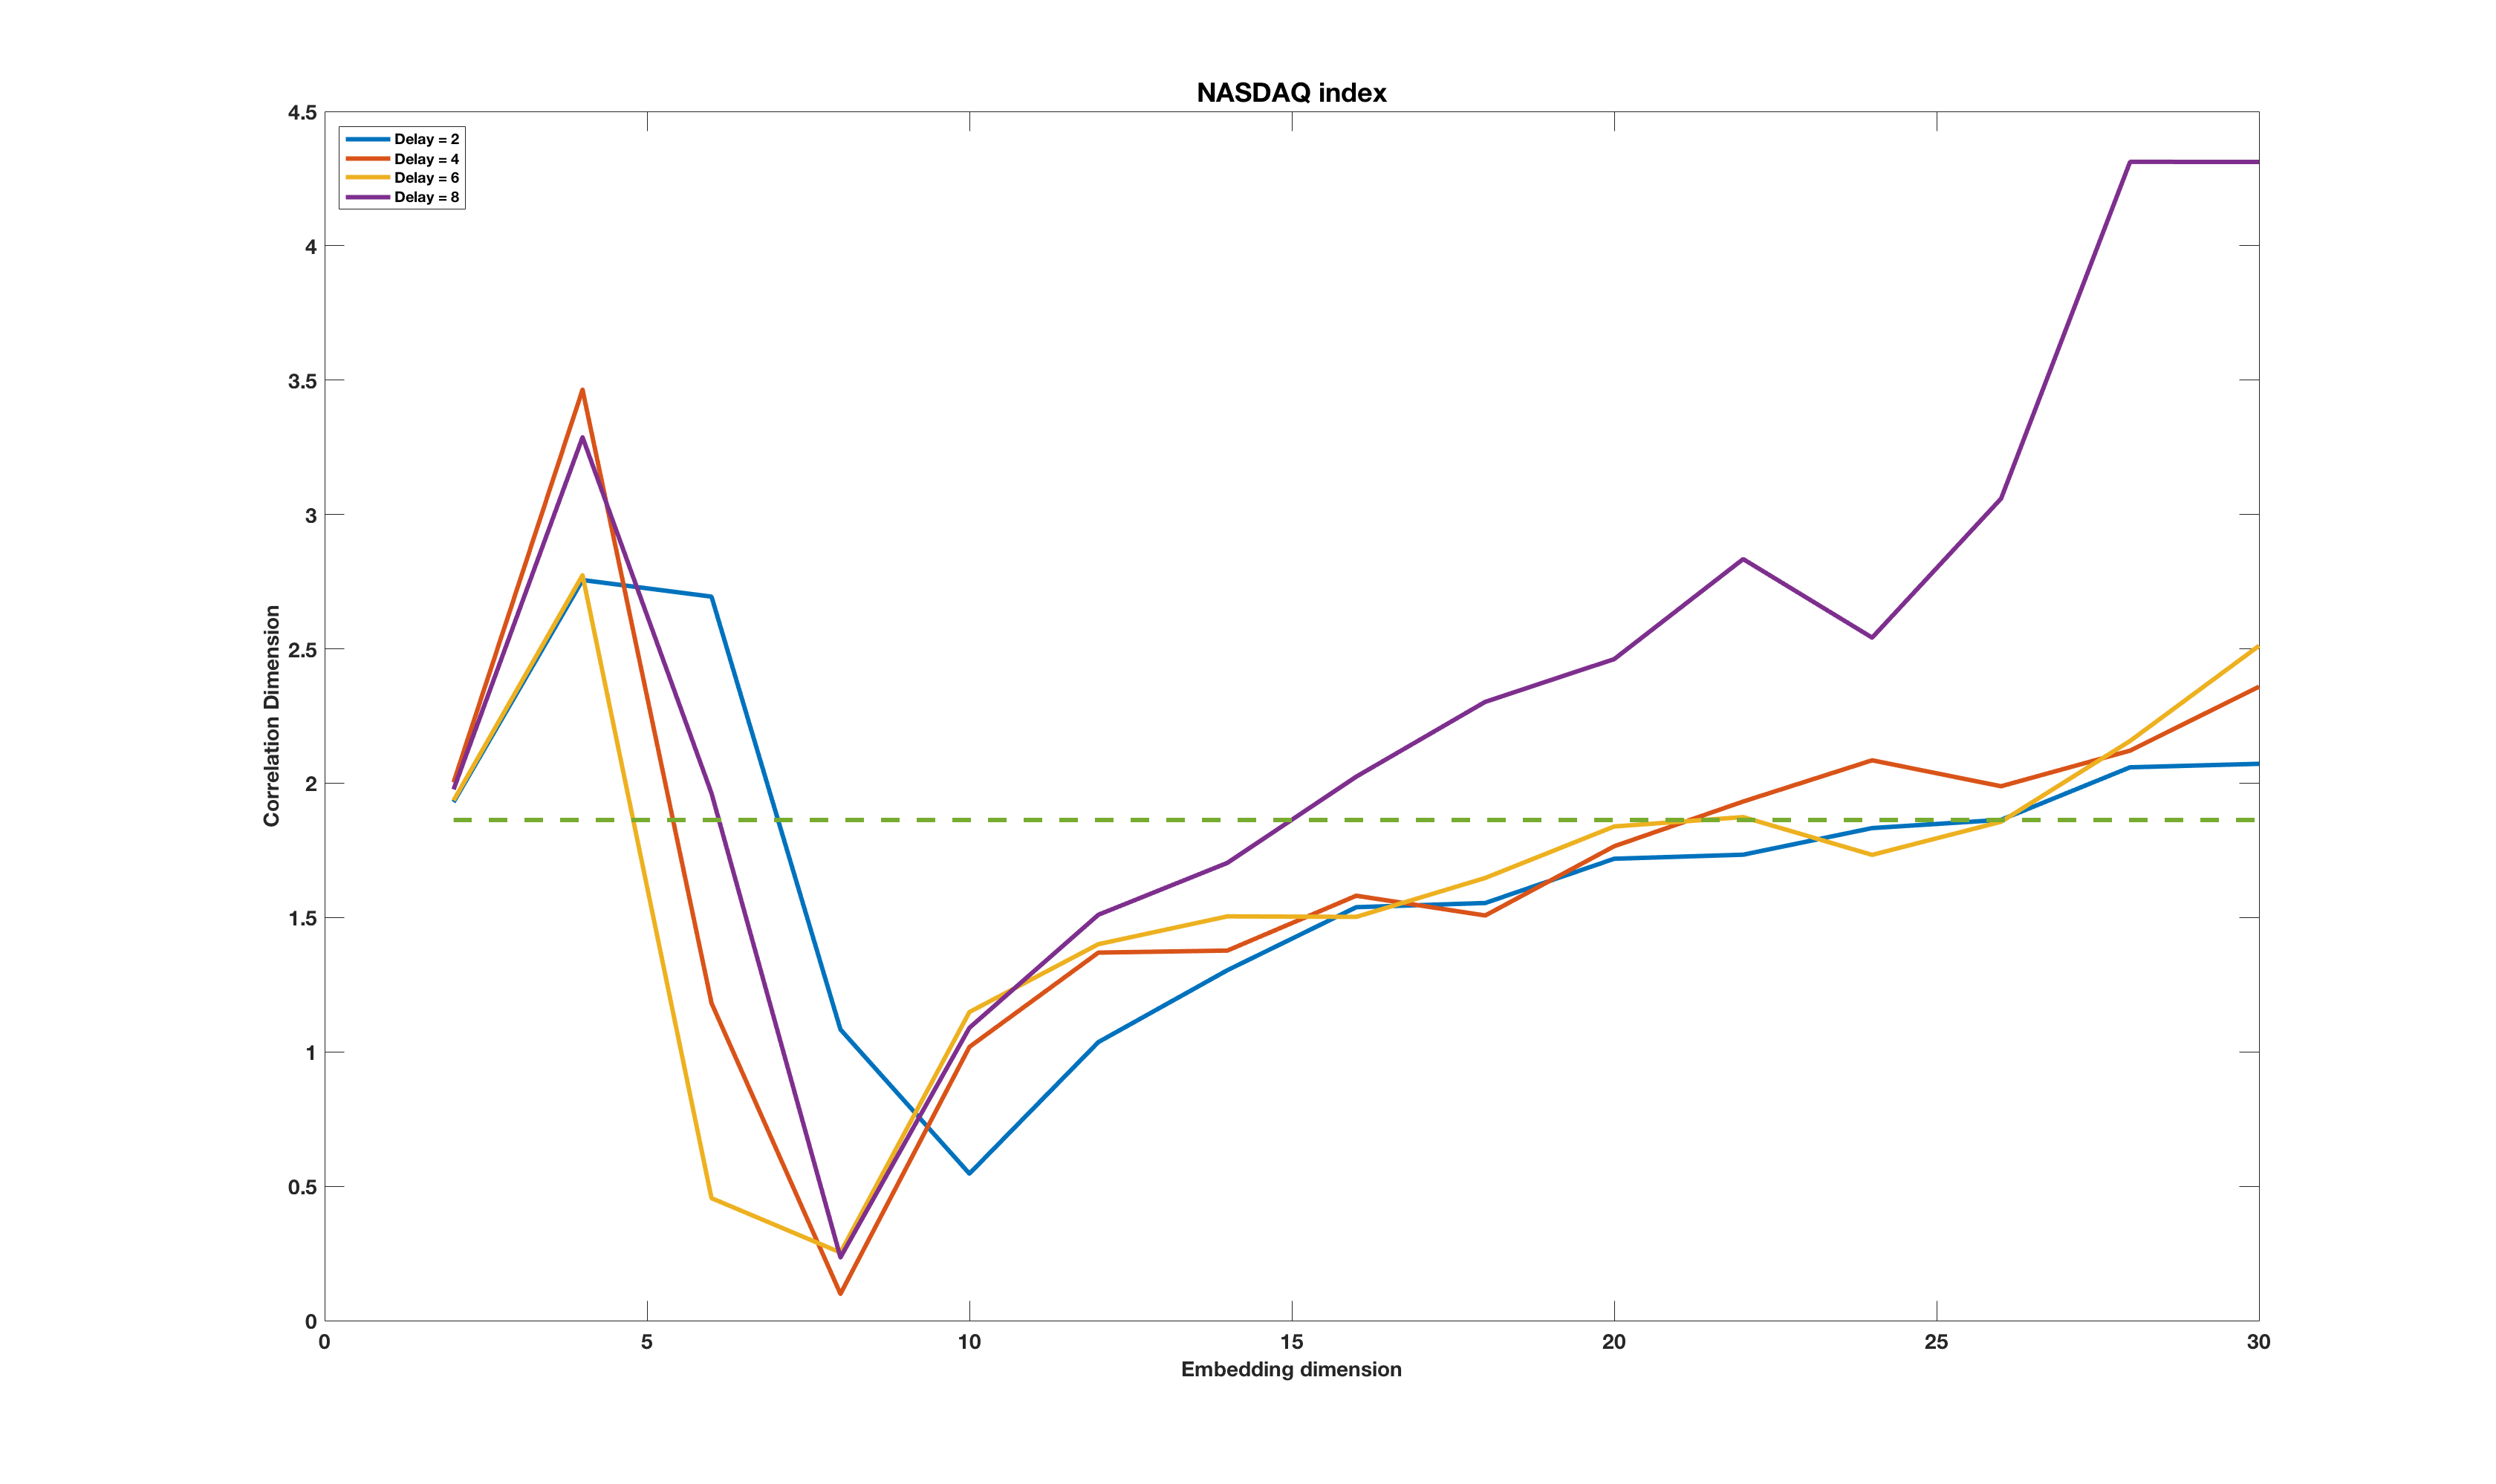
\includegraphics[scale=.15]{Images/NASDAQCD2}
\caption{Correlation Dimension for NASDAQ. The graph was created by using drawCorrDim.m and it is attached in the Appendix}
\label{fig:NASDAQCD2}
\end{figure}



\subsection{Lyapunov exponent}
The Lyapunov exponent is a quantity that describes the rate of separation of two neighbouring trajectories. The divergence of two trajectories at time $t$ with initial separation $\delta Z_0$ at $t=0$, is expressed as:

\begin{equation} \label{le:1}
|\delta Z(t)| \approx e^{\lambda t}|\delta Z_0|
\end{equation}
where $\lambda$ is the Lyapunov exponent. Different orientations of initial separation vectors would result in different rate of separation and thus, a whole spectrum of the Lyapunov exponents. The Largest $\lambda$ is called the Maximum Lyapunov Exponent: 

\begin{equation} \label{le:2}
%\lambda = lim_{t\to\infy} \frac{1}{t}
D_c = \lim_{\epsilon\to 0} \lim_{N\to\infty} \frac{\partial log_{10} C(\epsilon)}{\partial log_{10}(\epsilon)}
\end{equation}

%\lambda = lim_{t\to\infy} \frac{1}{t} ln \frac{|\delta Z(t)}|{\delta Z_0}

$\lambda gt 0$ is usually considered as indicator of chaos, $\lambda lt 0$ is usually considered an indicator of a mean reverting behavior and $\lambda = 0$ is a characteristic of cyclic behavior. 

\subsection{Instantaneous Autocorrelations and instantaneous frequency in Time-frequency representation}

The concepts of instantaneous autocorrelation and instantaneous frequency are important in developing generalized spectral analysis. A symmetric window in a localized time interval is introduced in the instantaneous autocorrelation function of the bilinear Wigner distribution (WD); the corresponding time-dependent frequency (or simply time frequency) can be defined by the Fourier spectrum of its autocorrelations. 

\begin{figure}[!ht]
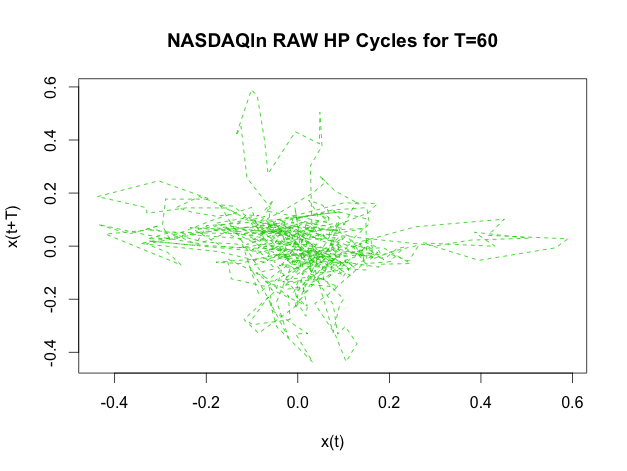
\includegraphics[scale=.7]{Images/NASDAQRawChaos}
\caption{Phase Portrait for log(NASDAQ) unfiltered series $T= 60$. The graph was created by using Attractor.R (R program) and it is attached in the Appendix A}
\label{fig:NASDAQRawChaos}
\end{figure}

\begin{figure}[!ht]
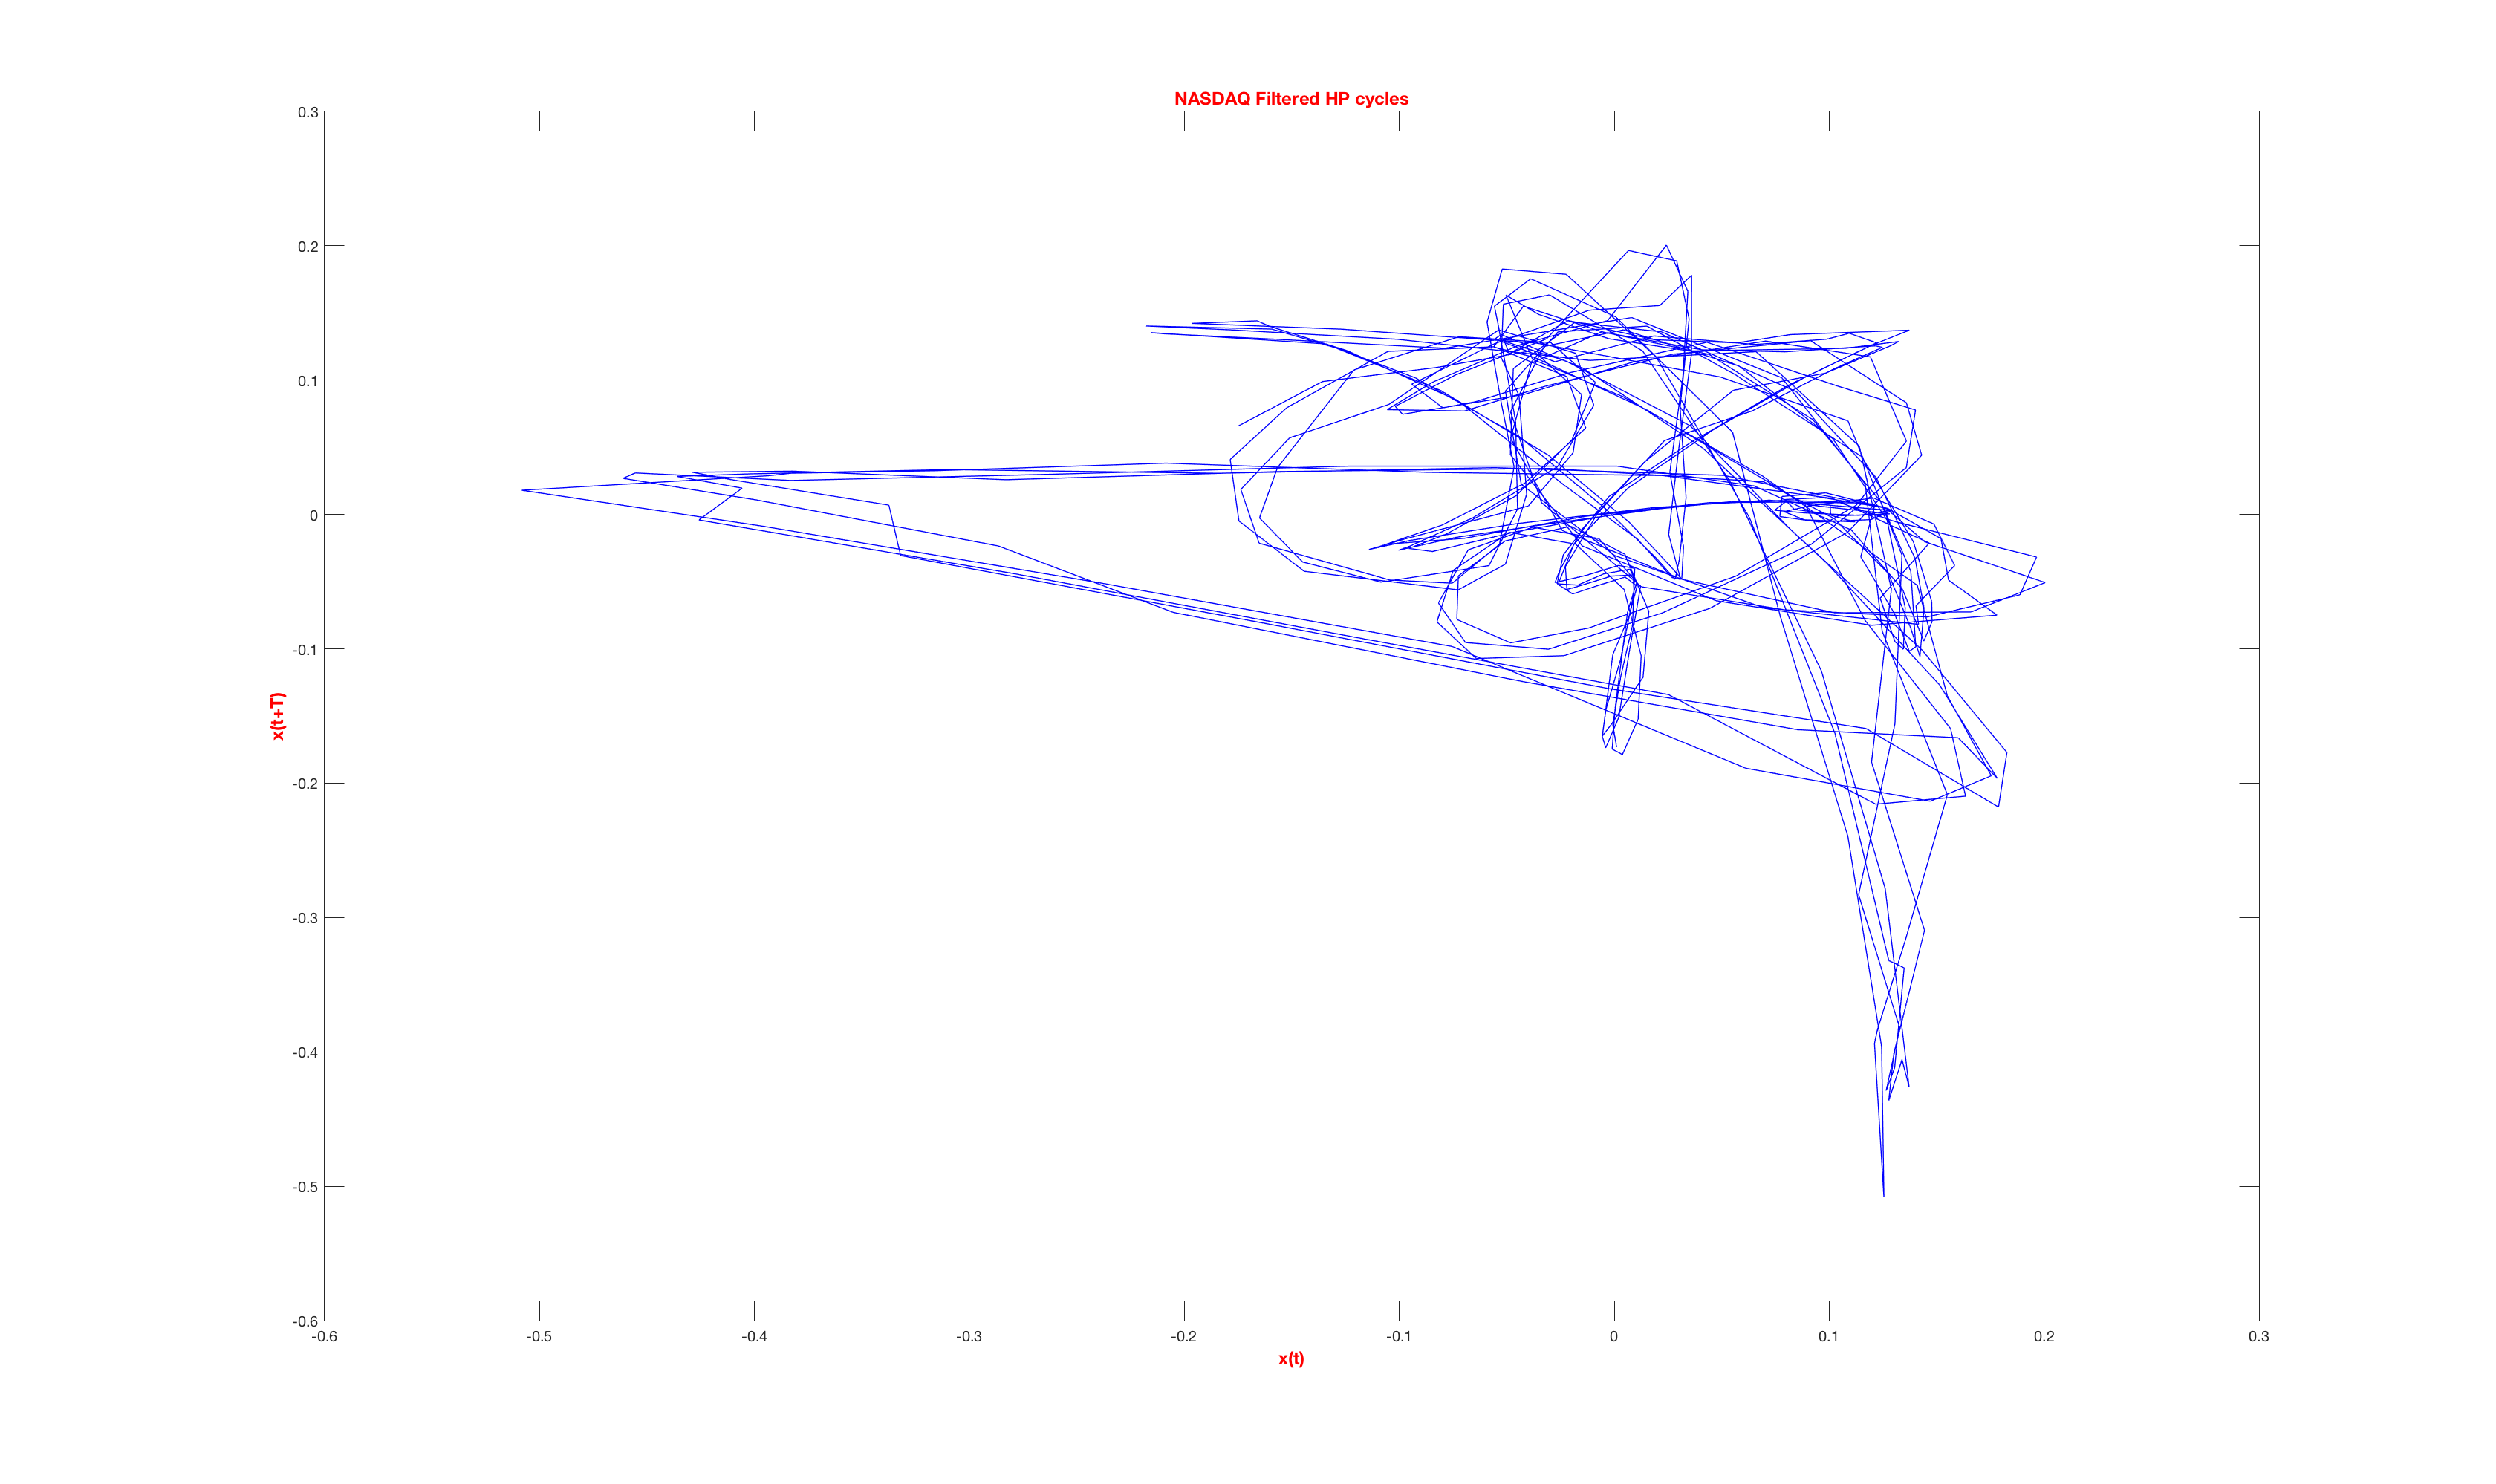
\includegraphics[scale=.15]{Images/NASFiltAttract}
\caption{Phase Portrait for log(NASDAQ) unfiltered series $T= 60$. A pattern of strange attractor can be observed in the graph. The threshold value that depends on $H$ $(H = 0.5)$ has less significant impact to the pattern emergence whereas the size of $m$, $n$ in $C(m,n)$, the Gabor Coefficient has significant impact to the pattern of strange attractor. The $16 x 16$ Gabor Coefficient was used. The graph was created by using myAttractor.m (Matlab program) and it is attached in the Appendix B.}
\label{fig:NASFiltAttract}
\end{figure}

\begin{figure}[!ht]
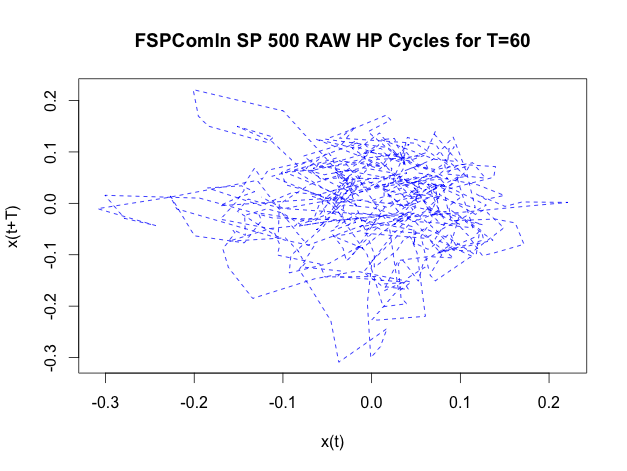
\includegraphics[scale=.7]{Images/SP500RawChaos}
\caption{Phase Portrait for log(SP500) unfiltered series $T= 60$. The graph was created by using Attractor.R (R program) and it is attached in the Appendix A.}
\label{fig:SP500RawChaos}
\end{figure}

\begin{figure}[!ht]
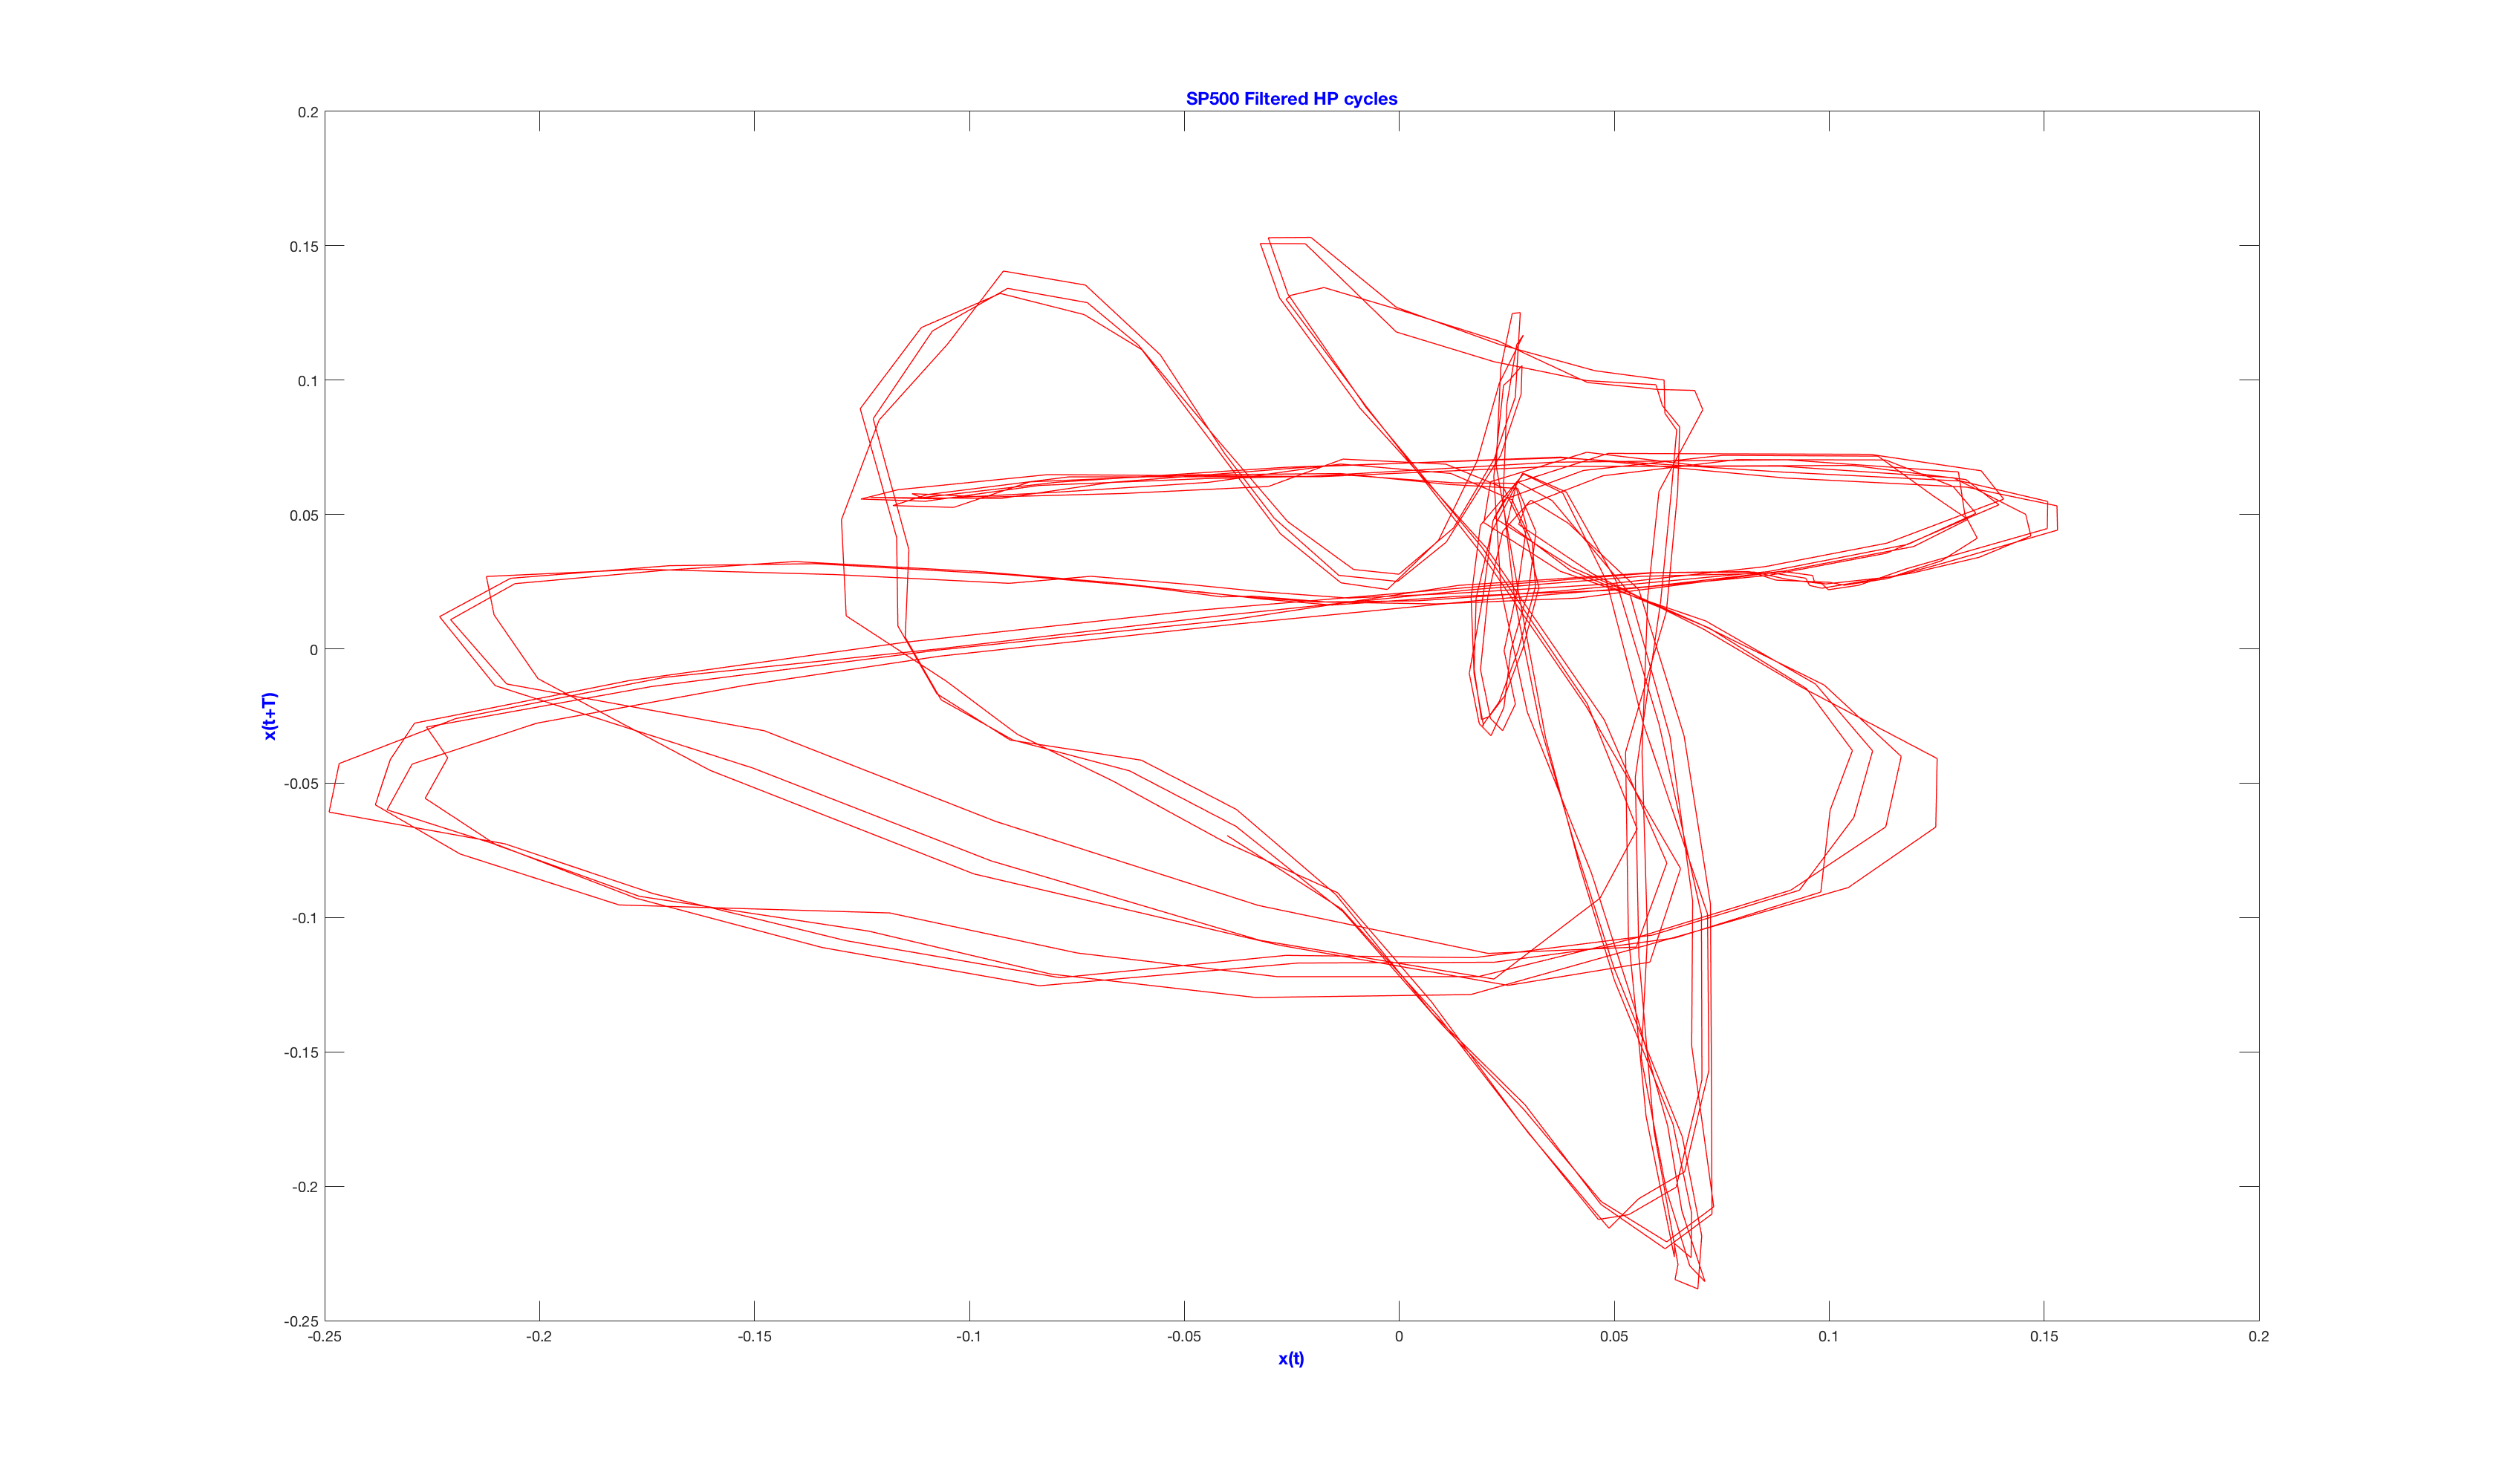
\includegraphics[scale=.15]{Images/SPFiltAttract}
\caption{Phase Portrait for log(SP500) unfiltered series $T= 60$. A pattern of strange attractor can be observed in the graph. The threshold value that depends on $H$ $(H = 0.5)$ has less significant impact to the pattern emergence whereas the size of $m$, $n$ in $C(m,n)$, the Gabor Coefficient has significant impact to the pattern of strange attractor. The $16 x 16$ Gabor Coefficient was used. The graph was created by using myAttractor.m (Matlab program) and it is attached in the Appendix B.}
\label{fig:SPFiltAttract}
\end{figure}

In the figure ~\ref{fig:SP500RawChaos} the chaos of the SP500 is shown and in the figure ~\ref{fig:NASDAQRawChaos} the chaos of the SP500 is shown.


\begin{figure}[!ht]
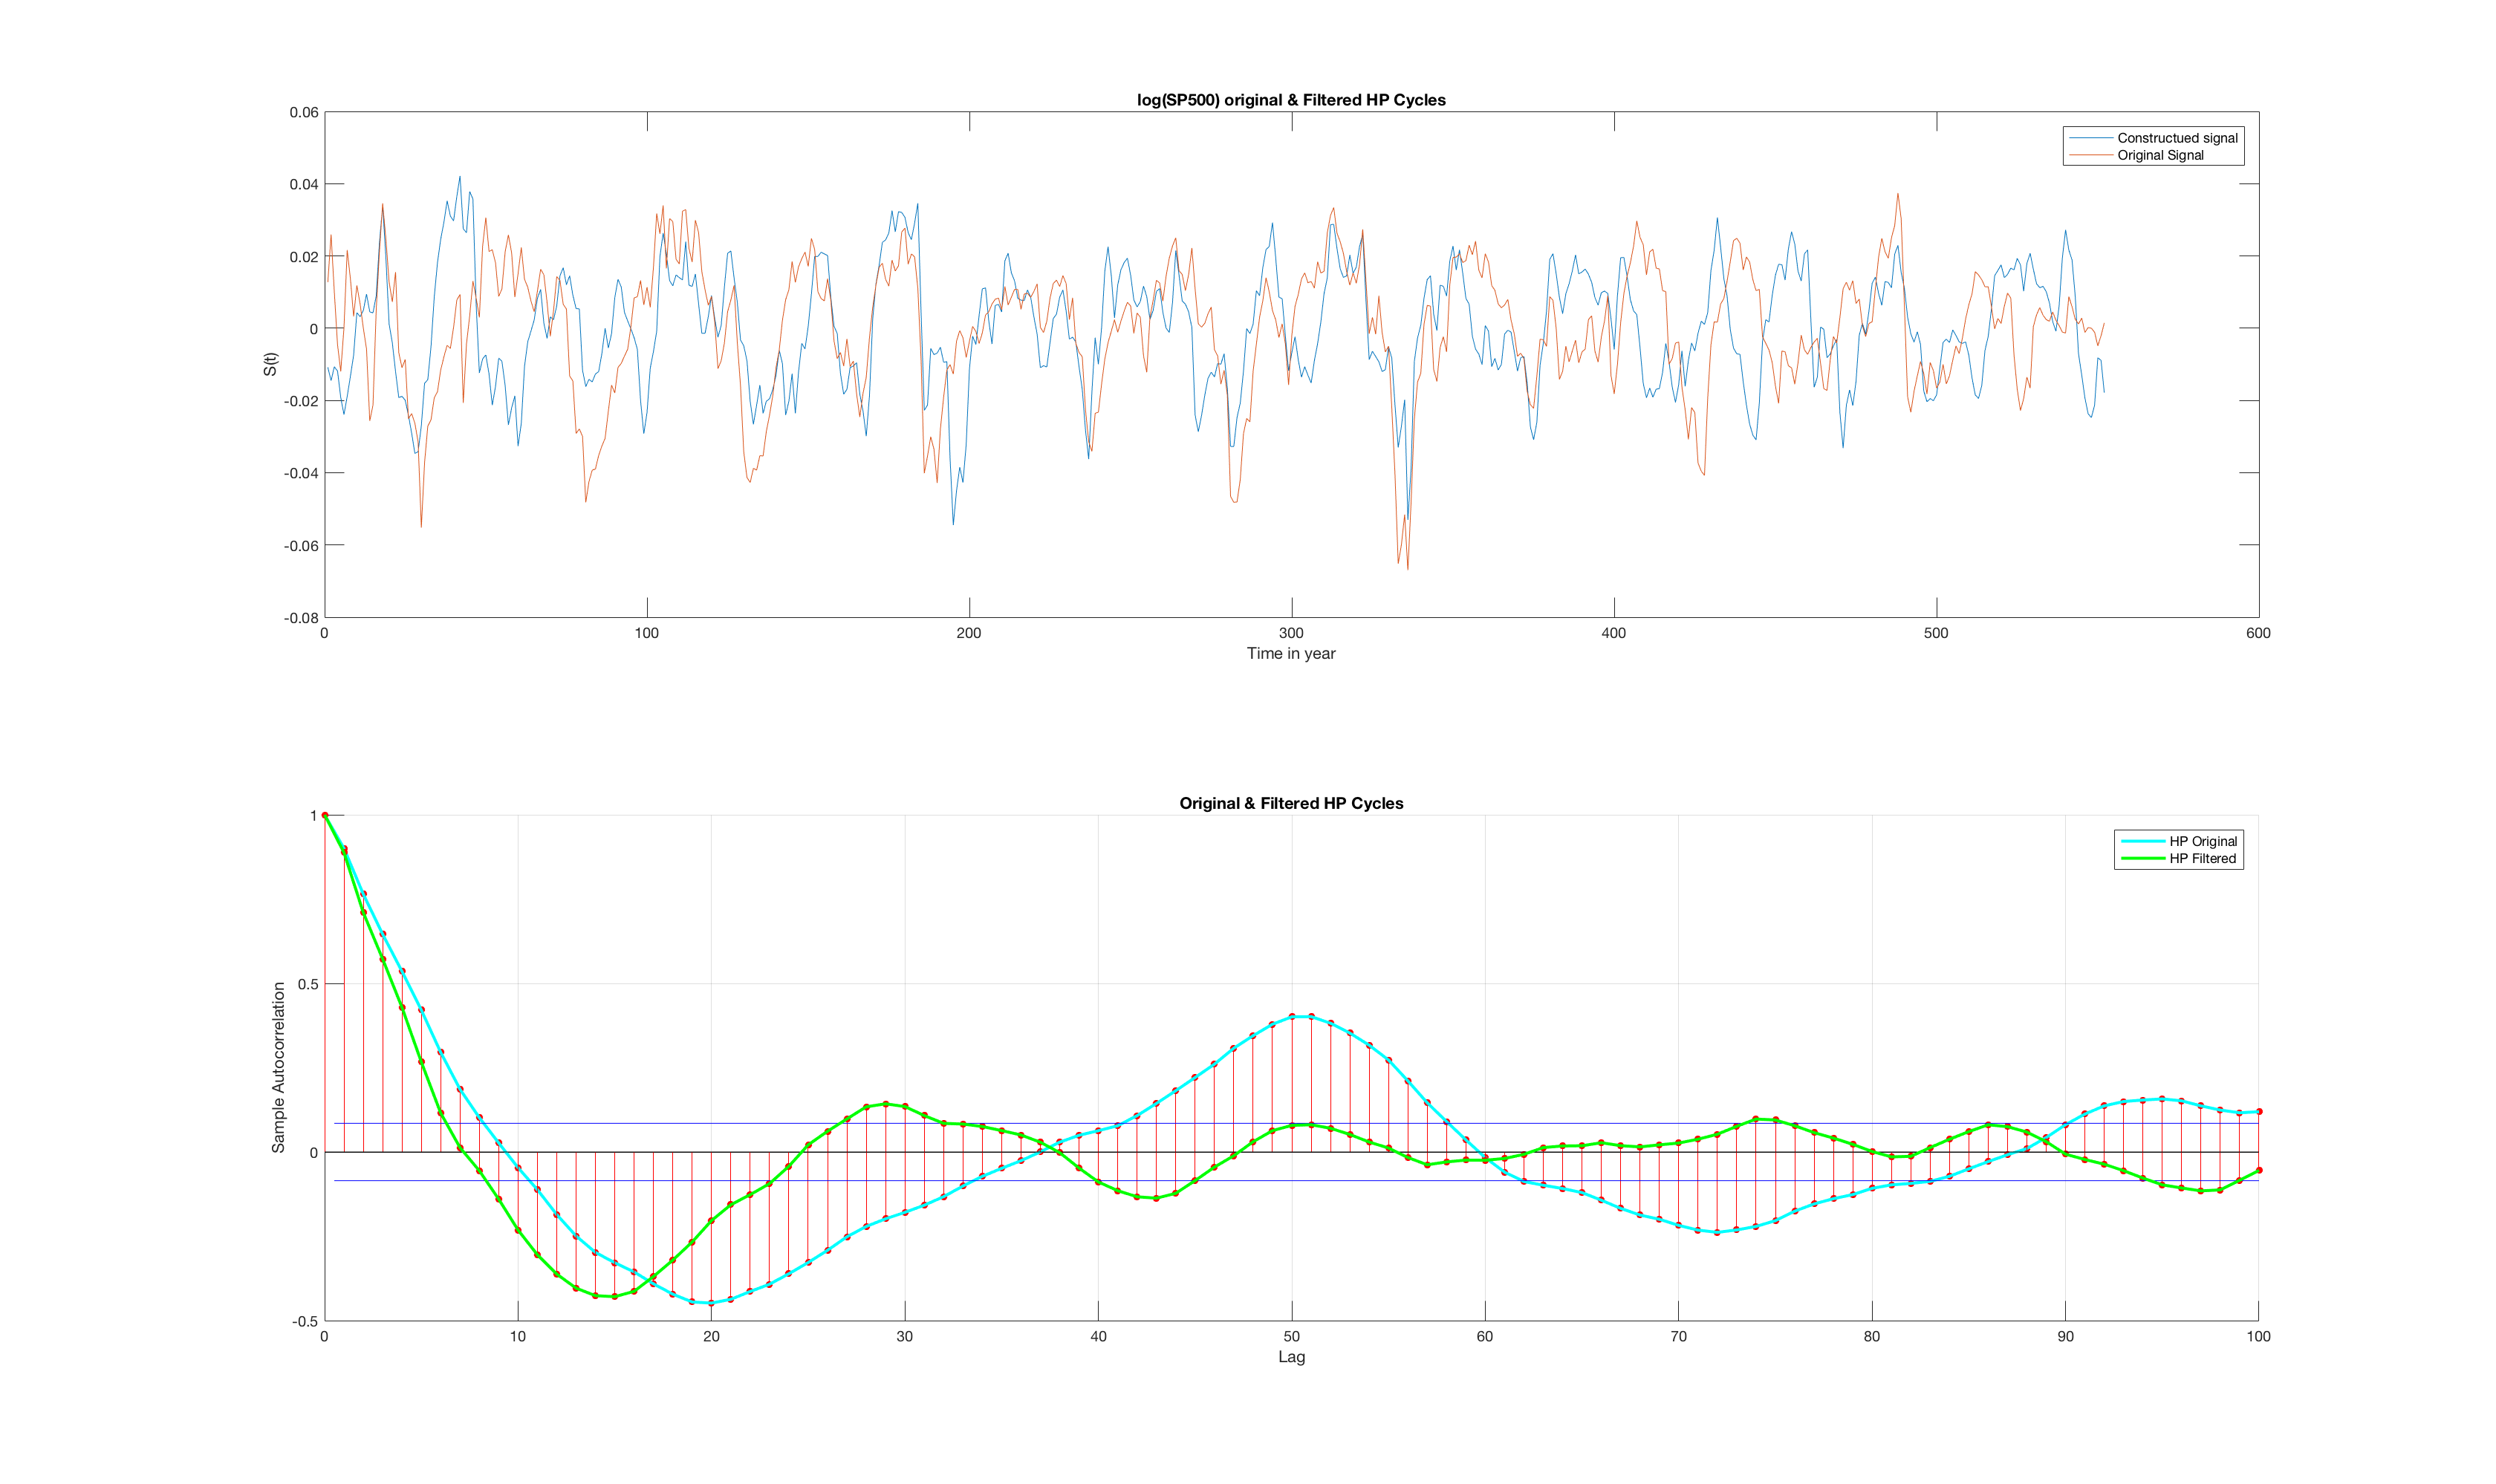
\includegraphics[scale=.15]{Images/SP500Recon}
\caption{Fig a) The original and reconstructed time series of log(SP500) HP Cycles. Gabor Coefficients are created using the parameters - .$\Delta M = 8; \Delta N = 4; m = 16; n = 16; \sigma = \sqrt{\frac{\Delta M L}{\Delta N 2\pi}}$. Fig b) Autocorelations of the original and reconstructed time series of log(SP500) HP cycle. The program used to create the graph is myreconstfromgabor.m and it is attached in the appendix B.}
\label{fig:SP500Recon}
\end{figure}

\begin{figure}[!ht]
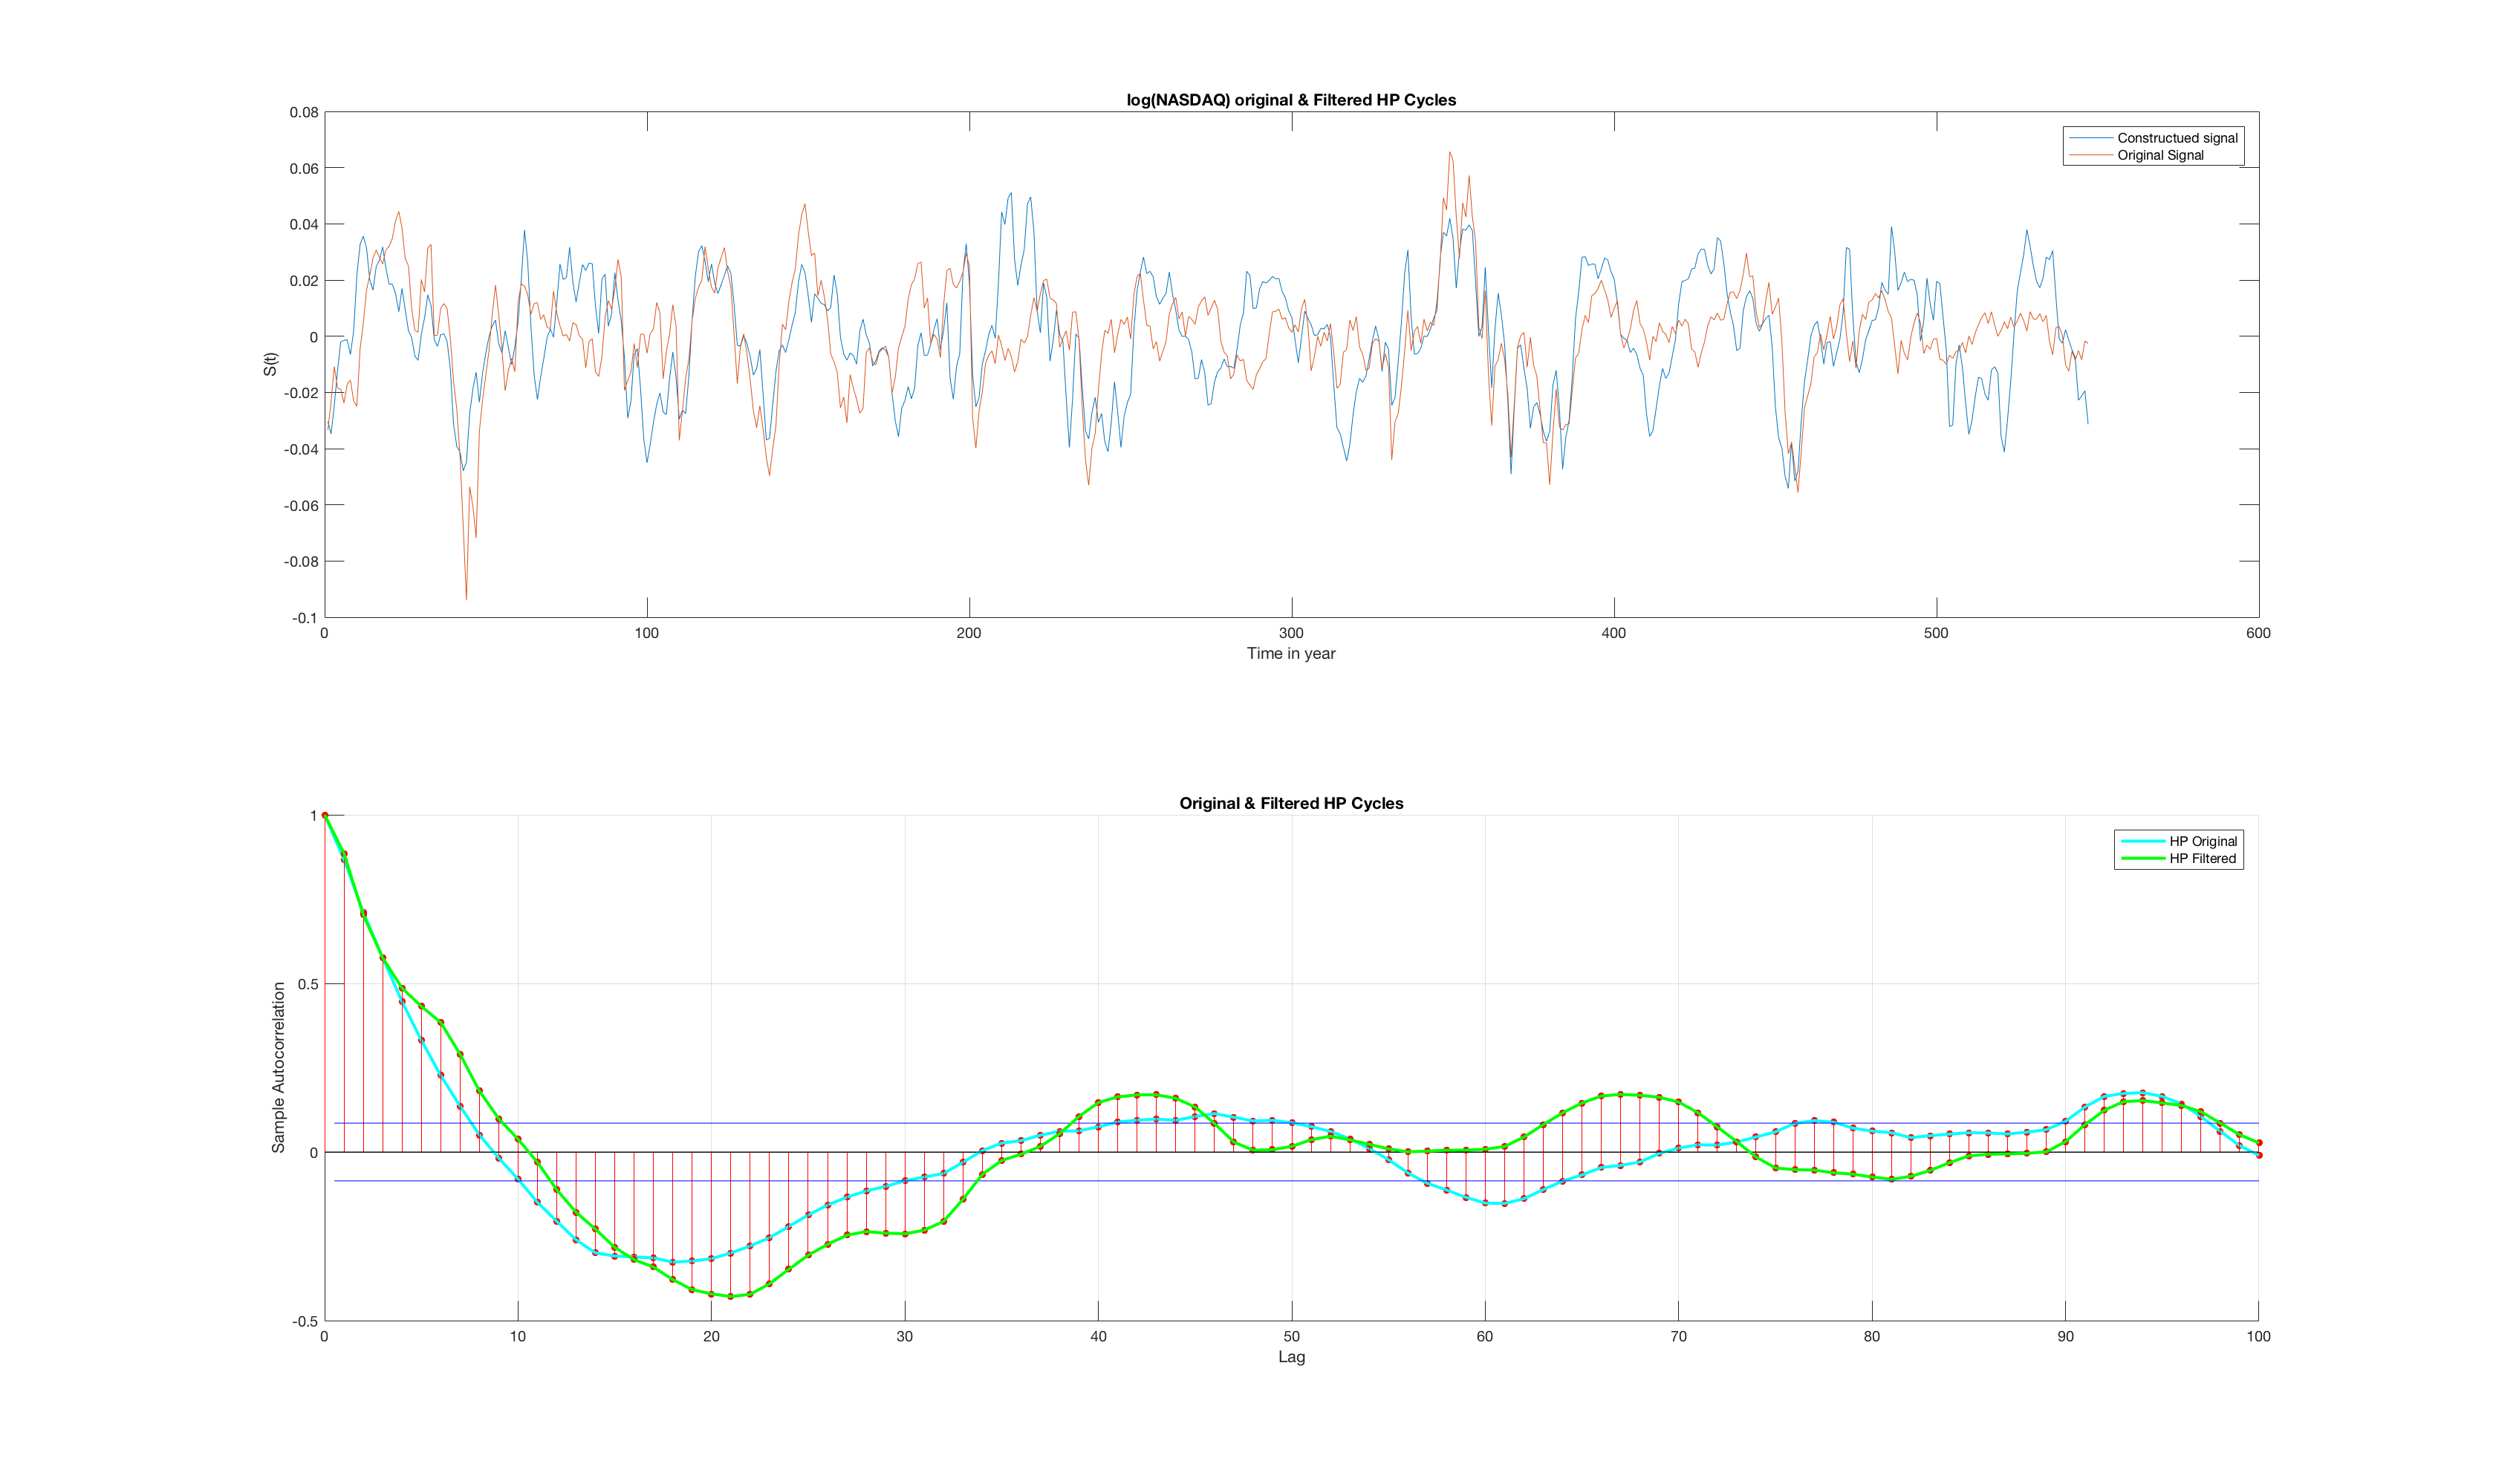
\includegraphics[scale=.15]{Images/NASRecon}
\caption{Fig a) The original and reconstructed time series of log(NASDAQ) HP Cycles. Gabor Coefficients are created using the parameters - .$\Delta M = 8; \Delta N = 4; m = 16; n = 16; \sigma = \sqrt{\frac{\Delta M L}{\Delta N 2\pi}}$. Fig b) Autocorelations of the original and reconstructed time series of log(NASDAQ) HP cycle. The program used to create the graph is myreconstfromgabor.m and it is attached in the appendix B.}
\label{fig:NASRecon}
\end{figure}

\begin{figure}[!ht]
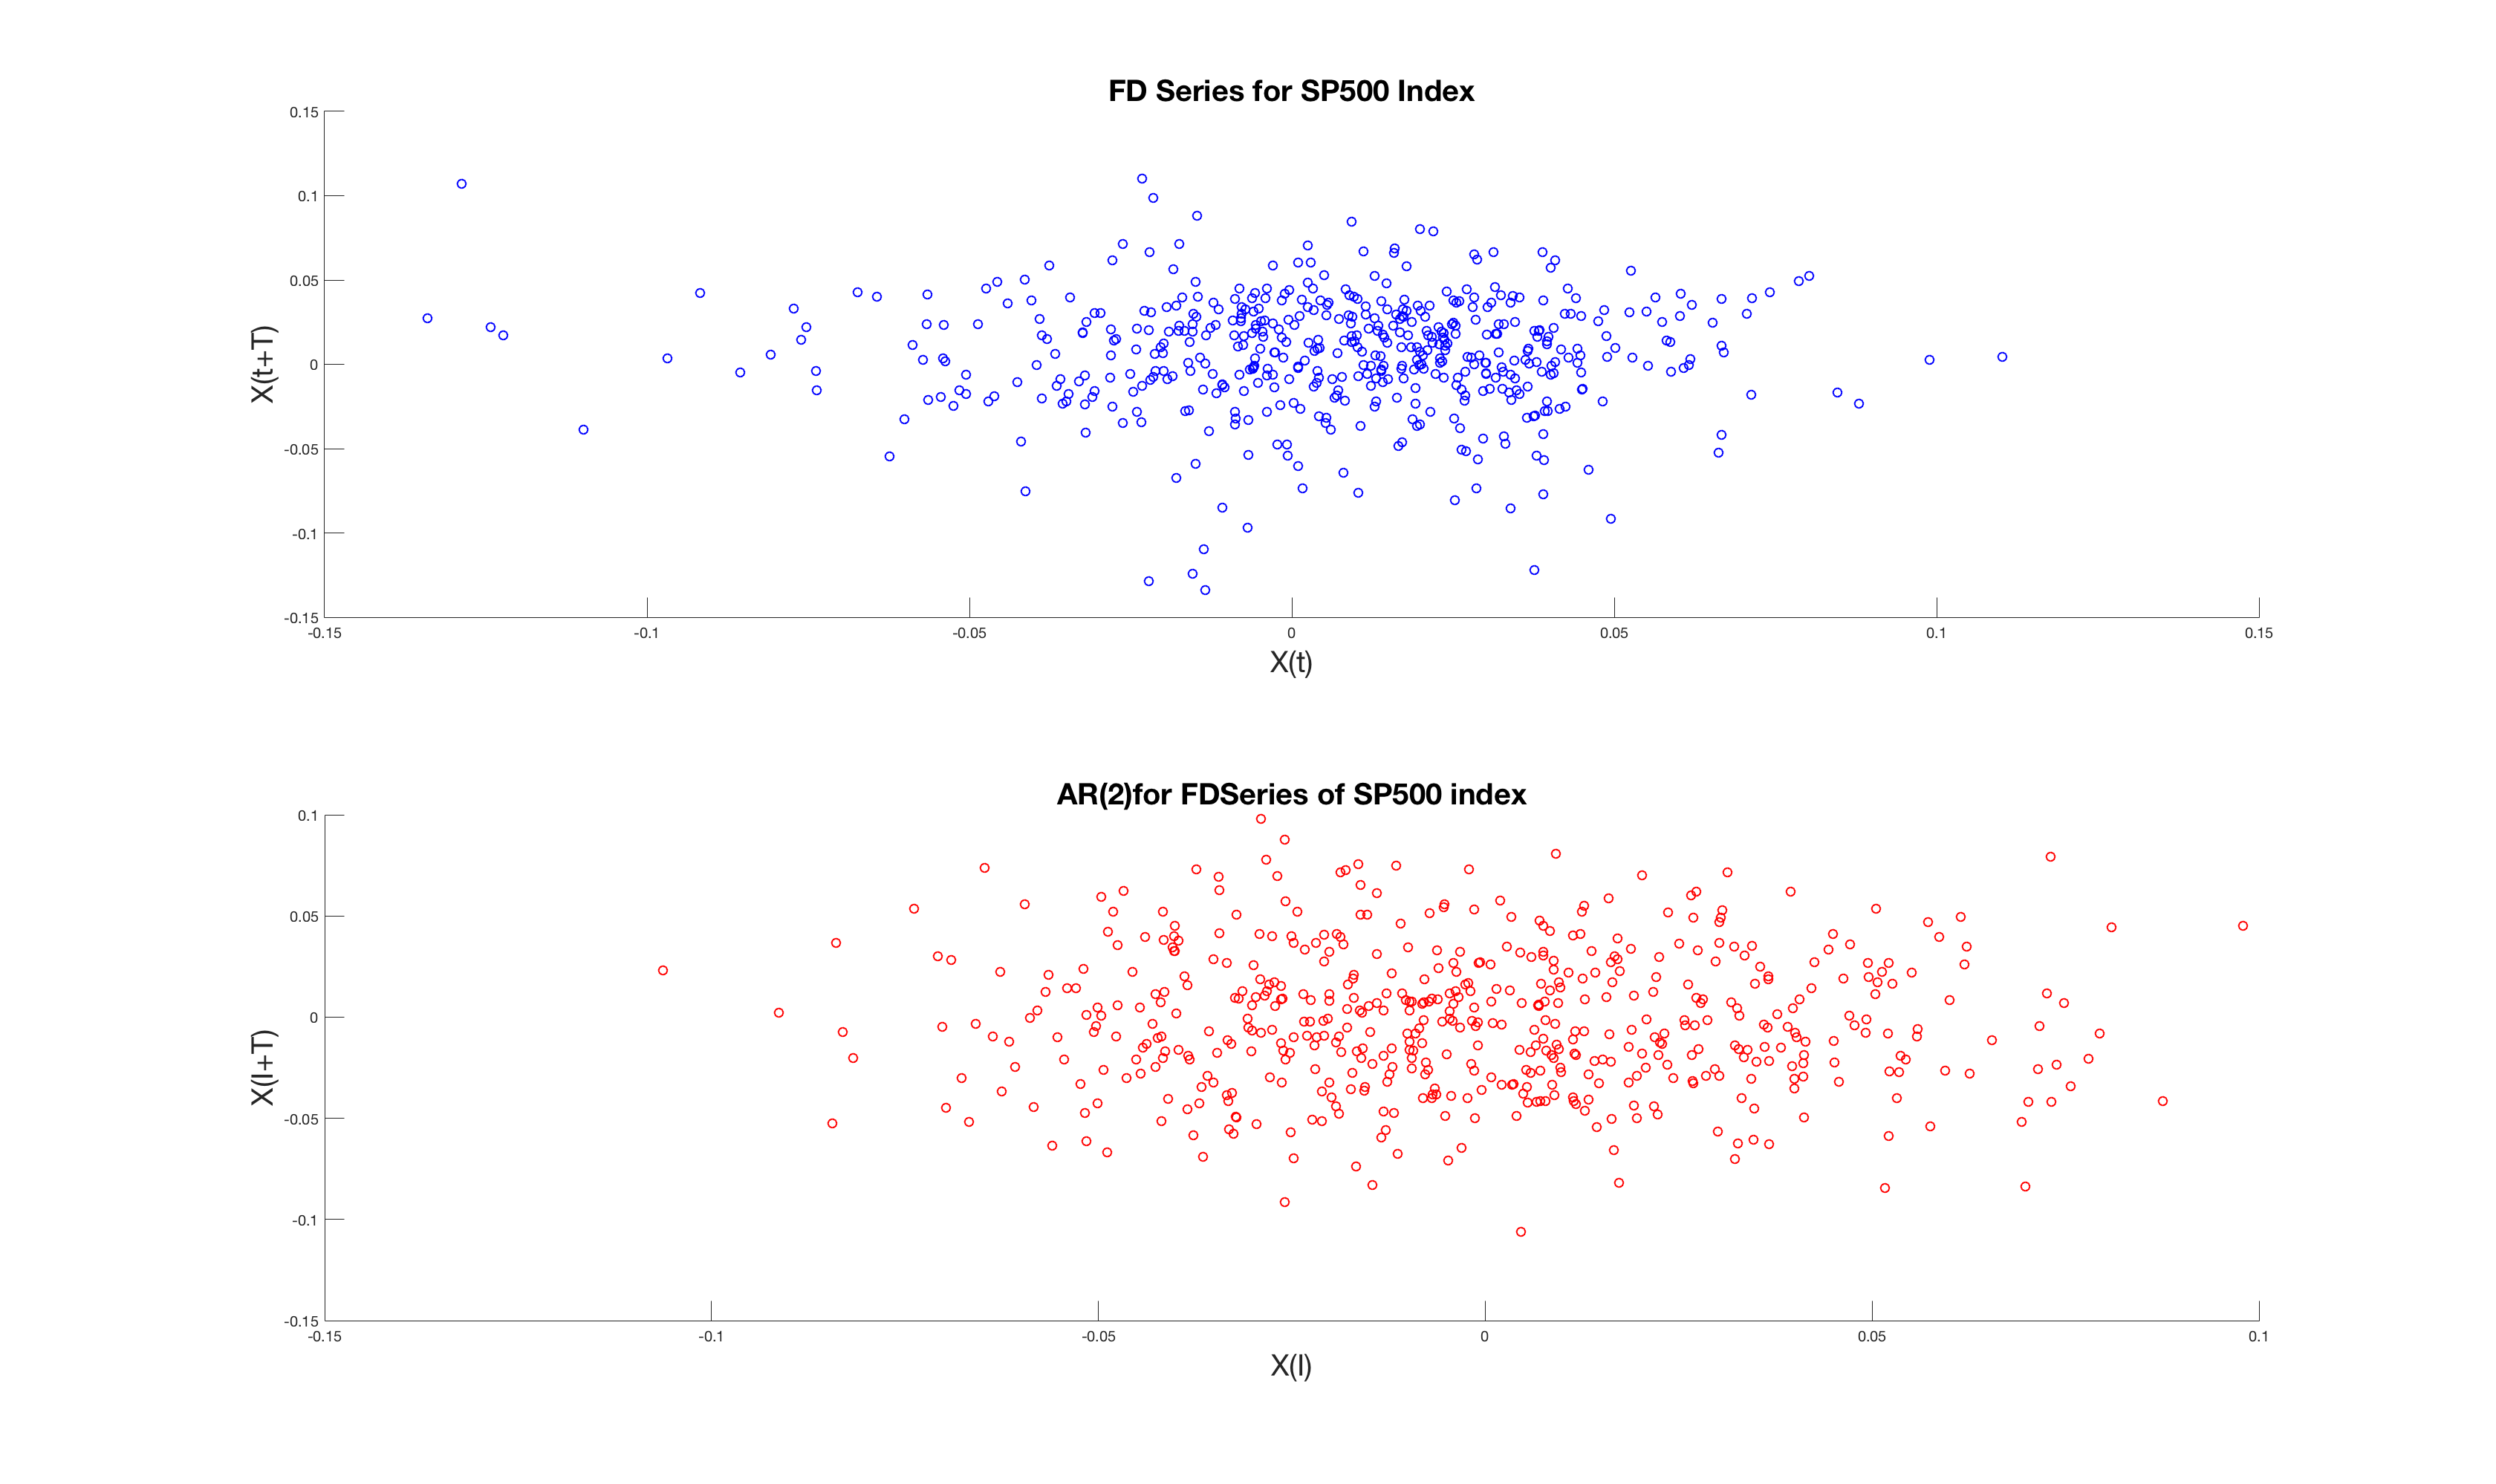
\includegraphics[scale=.15]{Images/FDAR2SP500}
\caption{Fig a) SP500 FD Series. T = 40. The pattern demonstrates the existence of dominant of high frequency noise. Fig b) AR(2) for the FD Series of SP500. T=5. The program used to create the graph is myFDFilter.m and it is attached in the appendix B.}
\label{fig:FDAR2SP500}
\end{figure}


\begin{figure}[!ht]
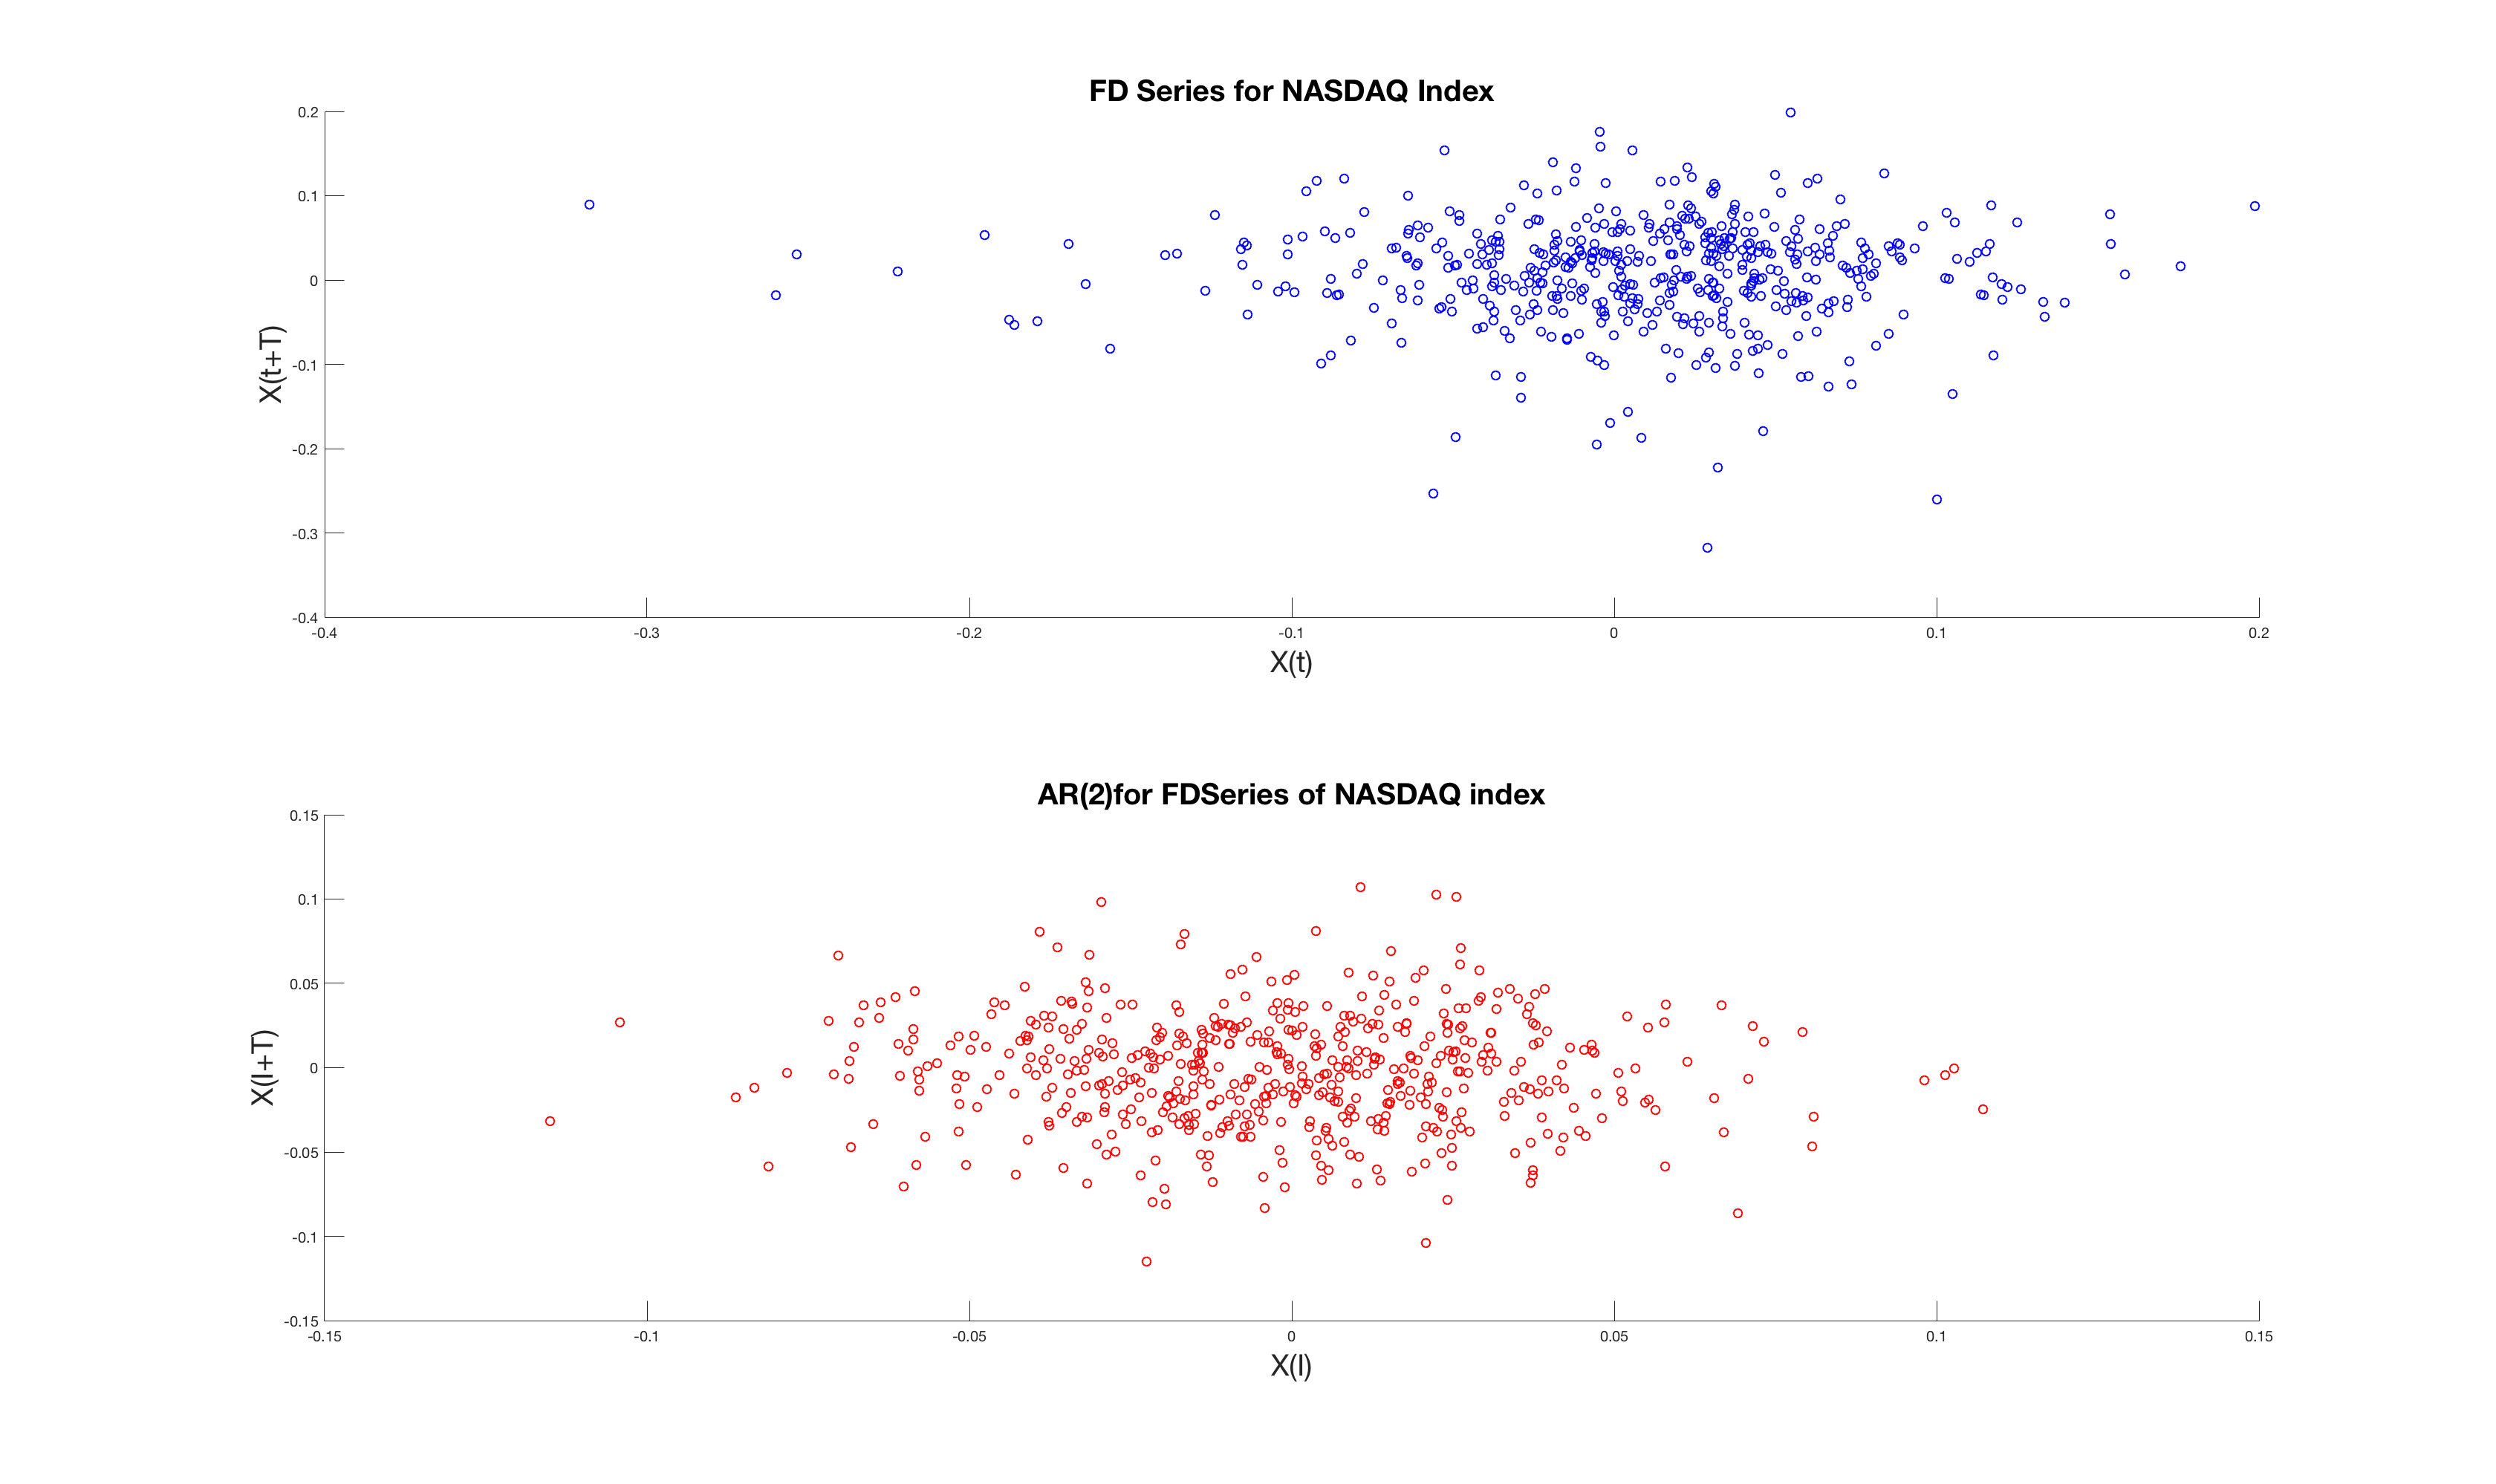
\includegraphics[scale=.15]{Images/FDAR2NASDAQ}
\caption{Fig a) NASDAQ FD Series. T = 40. The pattern demonstrates the existence of dominant of high frequency noise. Fig b) AR(2) for the FD Series of NASDAQ. T=5. The program used to create the graph is myFDFilter.m and it is attached in the appendix B.}
\label{fig:FDAR2NASDAQ}
\end{figure}

\begin{table}[h!]
\centering
\begin{tabular}{||c c c c c c c c c||}
 \hline
  Data & $\eta$ & $\nu(\%)$ & CCgo & $P_{c}$  & $\phi (\%)$ & $P_{dc}$ & $\lambda^{-1}$ &$\mu$ \\ [0.5ex]
   \hline\hline
    SP500 & 1.032 & 106.6 & 0.4141 & NA & NA & NA & NA\\
	 NASDAQ & 1.0116 & 102.33 & 0.4735 & NA & NA & NA & NA \\
	   \hline
	   \end{tabular}
	   \caption{Detrend Statistics on S\&P 500 }
	   \label{table:dectrendstat}
	   \end{table}
\subsection{Conclusion}
Color chaos model uncovers the business cycle in the stock market indices SP500 and NASDAQ and existence of persistent cycles reveals a new perspective of market. The study provides additional clarity on the opportunity in studying stock market movements using the joint time frequency analysis. A new study was performed by rearranging the indices value randomly instead of being time dependent, similar color chaos models was applied. The initial results of this new study revealed a similar cycles in the stock market. The results of this new study is not attached to this report but provides an opportunity to continue the study market behavior by converting the market indices value time independent. Further study may reveal more deeper understanding of the market behavior.



\startappendices
 \appendix{R code that are used to do analysis}
 %\begin{lstlisting}[basicstyle=\tiny,language=R]
hp_nasdaq <- function()
{
#Program used to create the HP filter for lambda 80 & 800 for NASDAQ index
#Load the file and invoke hp_nasdaq()
# Praba Siva;praba@umich.edu; @prabasiva
# R source
library(mFilter)
opar <- par(no.readonly=TRUE)
setwd("/Users/sivasp1/Documents/2016/Personal/Praba/MATH599/program")
dat <- read.csv(file="nasdaq_ready.csv",head=TRUE,sep=",")
year=dat[,1]+1/12*dat[,2]
dat=dat[,3]
ldat=log(dat)
dat=ldat
dat.hp1 <- hpfilter(dat, freq=80,type="frequency",drift=FALSE)
dat.hp2 <- hpfilter(dat, freq=800,type="frequency",drift=FALSE)
par(mfrow=c(3,1),mar=c(3,3,2,1),cex=.8)
plot(year,dat,  xlab="Year",ylab="log s(t)",ylim=range(dat),
     main="NASDAQ Index ",
     col=2, type='l')
plot(year,dat.hp1$trend,  xlab='Year', ylim=range(dat.hp1$trend),
     main="HP filter of NASDAQ Index: Trend,Lambda=80 ",
     col=4, type='l')
plot(year,dat.hp1$cycle,  ylim=range(dat.hp1$cycle), xlab="Year", 
     main="HP filter of NASDAQ Index: Cycle,Lambda=80 ",
     col=3, type='l')
par(mfrow=c(3,1),mar=c(3,3,2,1),cex=.8)
plot(year,dat,  ylim=range(dat),
     main="NASDAQ Index ",
     col=2, ylab="log s(t)",type='l')
plot(year,dat.hp2$trend,  ylim=range(dat.hp1$trend),
     main="HP filter of NASDAQ Index: Trend,Lambda=800 ",
     col=4, xlab='Year', ylab="log(s(t))",type='l')
plot(year,dat.hp1$cycle,  ylim=range(dat.hp2$cycle),
     main="HP filter of NASDAQ Index: Cycle,Lambda=800 ",
     col=3, ylab="",type='l')
par(opar)
}

hpfilt <- function()
{
#Program used to create the HP filter for lambda 80 & 800 for S&P 500 index
#Load the file and invoke hpfilt()
# Praba Siva;praba@umich.edu; @prabasiva
# R source
library(mFilter)
opar <- par(no.readonly=TRUE)
setwd("/Users/sivasp1/Documents/2016/Personal/Praba/MATH599/program")
fspcom=read.table('fspcom.dat')
dat = fspcom[,5]
year=fspcom[,2]+1/12*fspcom[,3]
ldat=log(dat)
dat=ldat
dat.hp1 <- hpfilter(dat, freq=80,type="frequency",drift=FALSE)
dat.hp2 <- hpfilter(dat, freq=800,type="frequency",drift=FALSE)
par(mfrow=c(3,1),mar=c(3,3,2,1),cex=.8)
plot(year,dat,  ylim=range(dat),
     main="S&P 500 Index ",
     col=2, ylab="",type='l')
plot(year,dat.hp1$trend,  ylim=range(dat.hp1$trend),
     main="HP filter of S&P 500 Index: Trend,Lambda=80 ",
     col=4, xlab='Year', ylab="log(s(t))",type='l')
plot(year,dat.hp1$cycle,  ylim=range(dat.hp1$cycle),
     main="HP filter of S&P 500 Index: Cycle,Lambda=80 ",
     col=3, ylab="",type='l')
par(mfrow=c(3,1),mar=c(3,3,2,1),cex=.8)
plot(year,dat,  ylim=range(dat),
     main="S&P 500 Index ",
     col=2, ylab="",type='l')
plot(year,dat.hp2$trend,  ylim=range(dat.hp1$trend),
     main="HP filter of S&P 500 Index: Trend,Lambda=800 ",
     col=4, xlab='Year', ylab="log(s(t))",type='l')
plot(year,dat.hp1$cycle,  ylim=range(dat.hp2$cycle),
     main="HP filter of S&P 500 Index: Cycle,Lambda=800 ",
     col=3, ylab="",type='l')
par(opar)

}
fdplot <-function()
{
  #Program used to create the Difference stationary for NASDAQ & SP500 indexes
  # Praba Siva
  # praba@umich.edu
  # @prabasiva
  setwd("/Users/sivasp1/Documents/2016/Personal/Praba/MATH599/program")
  fspcom=read.table('fspcom.dat')
  dat = log(fspcom[,5])
  year=fspcom[,2]+1/12*fspcom[,3]
  t1=dat[1:length(dat)-1]
  t2=dat[2:length(dat)]
  plot(year[1:length(year)-1],t2-t1,type='l',main="Difference stationary of first Differencing of log(x(t))\nx(t) = S&P 500", xlab="Year",ylab="FD",col=2,ylim=c(-.2,.2)) 
  
  setwd("/Users/sivasp1/Documents/2016/Personal/Praba/MATH599/program")
  dat <- read.csv(file="nasdaq_ready.csv",head=TRUE,sep=",")
  year=dat[,1]+1/12*dat[,2]
  dat=log(dat[,3])
  t1=dat[1:length(dat)-1]
  t2=dat[2:length(dat)]
  plot(year[1:length(year)-1],t2-t1,type='l',main="Difference stationary of first Differencing of log(x(t))\nx(t) = NASDAQ", xlab="Year",ylab="FD",col=3,ylim=c(-.2,.2)) 
  
}

llt<-function()
{
  #Program used to Log linear trend and cycles for SP500 & NASDAQ index
  # Praba Siva
  # praba@umich.edu
  # @prabasiva
setwd("/Users/sivasp1/Documents/2016/Personal/Praba/MATH599/program")
fspcom=read.table('fspcom.dat')
year=fspcom[,2]
tsfspcom=ts(log(fspcom[,5]),start=year[1],end=c(year[length(year)],12),frequency=12)
loglinear=stl(log(tsfspcom),s.window=5)
plot(loglinear,main="Log linear plot of S&P 500")

setwd("/Users/sivasp1/Documents/2016/Personal/Praba/MATH599/program")
dat <- read.csv(file="nasdaq_ready.csv",head=TRUE,sep=",")
year=dat[,1]
dat=dat[,3]
tsnasdaq=ts(dat,start=year[1],end=c(year[length(year)]-1,12),frequency=12)
nloglinear=stl(log(tsnasdaq),s.window=5)
plot(nloglinear,main="Log linear plot of NASDAQ")
}



\end{lstlisting}
\begin{lstlisting}[basicstyle=\tiny,language=MATLAB]


\end{lstlisting}

 \lstinputlisting[basicstyle=\tiny]{/Users/sivasp1/Documents/2016/Personal/Praba/Math599/program/fdplot.R}
\lstinputlisting[basicstyle=\tiny]{/Users/sivasp1/Documents/2016/Personal/Praba/Math599/program/llt.R}
\lstinputlisting[basicstyle=\tiny]{/Users/sivasp1/Documents/2016/Personal/Praba/Math599/program/hpfilter_slave.R}
\lstinputlisting[basicstyle=\tiny]{/Users/sivasp1/Documents/2016/Personal/Praba/Math599/program/loglinear.R}
\lstinputlisting[basicstyle=\tiny]{/Users/sivasp1/Documents/2016/Personal/Praba/Math599/program/AutoCorrelation.R}


 \appendix{Matlab code that are used to do analysis}
 \lstinputlisting[basicstyle=\tiny]{/Users/sivasp1/Documents/2017/Personal/program/DrawSinFourierGraph.m}
\lstinputlisting[basicstyle=\tiny]{/Users/sivasp1/Documents/2017/Personal/program/SPNASDAQFourier.m}
\lstinputlisting[basicstyle=\tiny]{/Users/sivasp1/Documents/2017/Personal/program/ghamwin.m}
\lstinputlisting[basicstyle=\tiny]{/Users/sivasp1/Documents/2017/Personal/program/drawSpecEg.m}
\lstinputlisting[basicstyle=\tiny]{/Users/sivasp1/Documents/2017/Personal/program/drawSpecEco.m}
\lstinputlisting[basicstyle=\tiny]{/Users/sivasp1/Documents/2017/Personal/program/drawSTFTECo3D.m}
\lstinputlisting[basicstyle=\tiny]{/Users/sivasp1/Documents/2017/Personal/program/stft2.m}
\lstinputlisting[basicstyle=\tiny]{/Users/sivasp1/Documents/2017/Personal/program/getData.m}
\lstinputlisting[basicstyle=\tiny]{/Users/sivasp1/Documents/2017/Personal/program/mywvd.m}
\lstinputlisting[basicstyle=\tiny]{/Users/sivasp1/Documents/2017/Personal/program/mywvdgauss.m}
\lstinputlisting[basicstyle=\tiny]{/Users/sivasp1/Documents/2017/Personal/program/mygabor.m}
\lstinputlisting[basicstyle=\tiny]{/Users/sivasp1/Documents/2017/Personal/program/myfiltgabor.m}
\lstinputlisting[basicstyle=\tiny]{/Users/sivasp1/Documents/2017/Personal/program/myreconsfromgabor.m}
\lstinputlisting[basicstyle=\tiny]{/Users/sivasp1/Documents/2017/Personal/program/myAttractor.m}
\lstinputlisting[basicstyle=\tiny]{/Users/sivasp1/Documents/2017/Personal/program/myFDfilter.m}
\lstinputlisting[basicstyle=\tiny]{/Users/sivasp1/Documents/2017/Personal/program/mydft.m}
\lstinputlisting[basicstyle=\tiny]{/Users/sivasp1/Documents/2017/Personal/program/drawCorrDim.m}
\lstinputlisting[basicstyle=\tiny]{/Users/sivasp1/Documents/2017/Personal/program/spectrumAnalysis5.m}
\lstinputlisting[basicstyle=\tiny]{/Users/sivasp1/Documents/2017/Personal/program/drawDataGraph.m}

 \appendix{Mathematical Proof}
 \section{Gabor Elementary function}
\begin{equation}
\psi(t) = \underbrace{e^{-\alpha ^2(t-t_0)^2}}_v\overbrace{e^{j2\pi f_0 t+\phi}}^w
\end{equation}

$v$ represents the probability function and $w$ represents simple harmonic oscillator.
$\Psi(f)$ is the GEF in the frequency domain. The GEF in the frequency domain is attained by taking the Fourier transform of the GEF.
\begin{equation*}
\Psi(f) = {\int_{-\infty}^{\infty}{\psi(t) e^{-j2\pi ft}dt}};
\Psi(f) = {\int_{-\infty}^{\infty}{e^{-\alpha ^2(t-t_0)^2}e^{j2\pi f_0 t+\phi} e^{-j2\pi ft}dt}}\\
\end{equation*}

\begin{equation*}
\Psi(f) = {\int_{-\infty}^{\infty}{e^{-\alpha ^2(t-t_0)^2}e^{j2\pi t(f_0-f) +\phi}dt}}
\end{equation*}

\begin{equation*}
\Psi(f) = e^\phi{\int_{-\infty}^{\infty}{e^{-\alpha ^2(t-t_0)^2}e^{j2\pi t(f_0-f) }dt}}
\end{equation*}

when $t_0$ is 0, then

\begin{equation}
\Psi(f) = e^\phi{\int_{-\infty}^{\infty}{e^{-\alpha ^2 t^2}e^{j2\pi t(f_0-f) }dt}}
\end{equation}


This is of the form.
\begin{equation*}
\int_{-\infty}^{\infty}e^{2bx - ax^2 }dx = \sqrt{\frac{\pi}{a}} e^\frac{b^2}{a}
\end{equation*}
where $b = j \pi(f_0-f)$ and $a = \alpha ^ 2$

\begin{equation*}
\Psi(f) = \sqrt{\frac{\pi}{\alpha ^2}} e^\frac{{(j\pi (f_0-f))}^2}{\alpha ^2}e^\phi
\end{equation*}
\begin{equation*}
\Psi(f) = \sqrt{\frac{\pi}{\alpha ^2}} e^{-{(\frac{\pi} {\alpha}})^2 ({f_0-f})^2+\phi}
\end{equation*}
$\alpha$ is connecting the GEF between time and frequency domain. $\psi(t)$ and $\Psi(f)$ occupies the minimum uncertainty in time and frequency domain.


\subsection{Proof: GEF has minimum uncertainty in the time-frequency domain}

I believe, we will better understand physical or mathematical concept by performing a step wise derivation. Let me do a step wise derivation to prove that GEF has a minimum uncertainty for a special case. Let me simplify the GEF by taking GEF at zero frequency, $t_0 = 0$ and $\phi = 0$,the Gabor elementary function and Fourier transform of GEF are given by
\begin{equation*}
\psi(t) = e^{-\alpha ^2 t^2}
\end{equation*}

\begin{equation*}
\Psi(f) = \sqrt{\frac{\pi}{\alpha ^2}} e^{-{(\frac{\pi} {\alpha}})^2 f^2}
\end{equation*}

Effective duration $\Delta t$ is given by:

\begin{equation*}
\Delta t = \sqrt{\frac{\int_{-\infty}^{\infty}{e^{-\alpha ^2 t^2} t^2  e^{-\alpha ^2 t^2} dt}}{\int_{-\infty}^{\infty}{e^{-\alpha ^2 t^2} e^{-\alpha ^2 t^2}dt}}} ;
\end{equation*}

Let me take the denominator first

\begin{equation*}
\int_{-\infty}^{\infty}{e^{-\alpha ^2 t^2} e^{-\alpha ^2 t^2}dt} =\int_{-\infty}^{\infty}{e^{-2\alpha ^2 t^2} dt}
\end{equation*}

The above equation is of the form and it only applies when $a > 0$

\begin{equation*}
\int_{-\infty}^{\infty}e^{-ax^2 }dx = \sqrt{\frac{\pi}{a}}
\end{equation*}

where $a = 2\alpha ^ 2$

\begin{equation*}
\int_{-\infty}^{\infty}{e^{-2\alpha ^2 t^2} dt} = \sqrt{\frac{\pi}{2\alpha ^ 2}}
\end{equation*}

Let me take the numerator now,

\begin{equation*}
\int_{-\infty}^{\infty}{e^{-\alpha ^2 t^2} t^2 e^{-\alpha ^2 t^2}dt} =\int_{-\infty}^{\infty}{t^2 e^{-2\alpha ^2 t^2} dt}
\end{equation*}

The above equation is of the form.
\begin{equation*}
\int_{-\infty}^{\infty}x^2 e^{- ax^2 }dx = \frac{1}{2}\sqrt{\frac{\pi}{a^3}}
\end{equation*}
where $a = 2\alpha ^ 2$
\begin{equation*}
\int_{-\infty}^{\infty}{t^2 e^{-2\alpha ^2 t^2} dt} = \frac{1}{2} \sqrt{\frac{\pi}{({2\alpha ^2})^3}} = \frac{\sqrt{\pi}}{4 \sqrt{2}\alpha ^3}
\end{equation*}

Let me apply both numerator and denominator value to get the effective duration $\Delta t$

\begin{equation*}
\Delta t = \sqrt{\frac{\frac{\sqrt{\pi}}{4 \sqrt{2}\alpha ^3}}{\sqrt{\frac{\pi}{2\alpha ^ 2}}}} ;
\end{equation*}

Straight forward steps to simply the value of $\Delta t$

\begin{equation*}
\Delta t =  \sqrt{\frac{\sqrt{\pi}}{4 \sqrt{2}\alpha ^3}{\sqrt{\frac{2\alpha ^ 2}{\pi}}}} ;
\end{equation*}

\begin{equation*}
\Delta t =  \sqrt{\frac{\sqrt{\pi}}{4 \sqrt{2}\alpha ^3}{\sqrt{\frac{2\alpha ^ 2}{\pi}}}} ;
\end{equation*}

\begin{equation*}
\Delta t =  \sqrt{\frac{1}{4 \alpha ^2}};
\end{equation*}


\begin{equation}
\Delta t =  \frac{1}{2 \alpha }
\end{equation}

Let me do the similar steps to calculate the effective frequency $\Delta f$. The frequency representation of the GEF is given by,

\begin{equation*}
\Psi(f) = \sqrt{\frac{\pi}{\alpha ^2}} e^{-{(\frac{\pi} {\alpha}})^2 f^2}
\end{equation*}

Effective frequency $\Delta f$ is given by,

\begin{equation*}
\Delta f = \sqrt{\frac{\int_{-\infty}^{\infty}{\sqrt{\frac{\pi}{\alpha ^2}} e^{-{(\frac{\pi} {\alpha}})^2 f^2} f^2 \sqrt{\frac{\pi}{\alpha ^2}} e^{-{(\frac{\pi} {\alpha}})^2 f^2} df}}{\int_{-\infty}^{\infty}{\sqrt{\frac{\pi}{\alpha ^2}} e^{-{(\frac{\pi} {\alpha}})^2 f^2}  \sqrt{\frac{\pi}{\alpha ^2}} e^{-{(\frac{\pi} {\alpha}})^2 f^2} df}}} ;
\end{equation*}

Let me take the denominator first.


\begin{equation*}
\int_{-\infty}^{\infty}{\sqrt{\frac{\pi}{\alpha ^2}} e^{-{(\frac{\pi} {\alpha}})^2 f^2}  \sqrt{\frac{\pi}{\alpha ^2}} e^{-{(\frac{\pi} {\alpha}})^2 f^2} df} = \frac{\pi}{\alpha ^2} \int_{-\infty}^{\infty}{ e^{-2{(\frac{\pi} {\alpha}})^2 f^2}df}
\end{equation*}



The above equation is of the form and it only applies when $a > 0$

\begin{equation*}
\int_{-\infty}^{\infty}e^{-ax^2 }dx = \sqrt{\frac{\pi}{a}}
\end{equation*}

where $a = 2(\frac{\pi}{\alpha})^ 2$

\begin{equation*}
\frac{\pi}{\alpha ^2} \int_{-\infty}^{\infty}{ e^{-2{(\frac{\pi} {\alpha}})^2 f^2}df} = \frac{\pi}{\alpha ^2} \sqrt{\frac{\pi}{2(\frac{\pi}{\alpha})^ 2}}
\end{equation*}

Let $\beta = \frac{\pi}{\alpha}$
\begin{equation*}
\frac{\pi}{\alpha ^2} \int_{-\infty}^{\infty}{ e^{-2{(\frac{\pi} {\alpha}})^2 f^2}df} = \frac{\beta}{\alpha} \sqrt{\frac{\pi}{2 \beta^ 2}} = \frac{1}{\alpha} \sqrt{\frac{\pi}{2 }}
\end{equation*}
Let me take the numerator now.
\begin{equation*}
\int_{-\infty}^{\infty}{\sqrt{\frac{\pi}{\alpha ^2}} e^{-{(\frac{\pi} {\alpha}})^2 f^2} f^2  \sqrt{\frac{\pi}{\alpha ^2}} e^{-{(\frac{\pi} {\alpha}})^2 f^2} df}
\end{equation*}

\begin{equation*}
=\frac{\pi}{\alpha ^2}\int_{-\infty}^{\infty}{ f^2 e^{-2{(\frac{\pi} {\alpha}})^2 f^2}  df}
\end{equation*}

Substitute $\beta$ in above equation.

\begin{equation*}
=\frac{\beta}{\alpha }\int_{-\infty}^{\infty}{ f^2 e^{-2 \beta ^2 f^2}  df}
\end{equation*}


The above equation is of the form.
\begin{equation*}
\int_{-\infty}^{\infty}x^2 e^{- ax^2 }dx = \frac{1}{2}\sqrt{\frac{\pi}{a^3}}
\end{equation*}
where $a = 2\beta ^ 2$
\begin{equation*}
 = \frac{\beta}{\alpha}\frac{1}{2}\sqrt\frac{\pi}{8\beta ^6 }
\end{equation*}

\begin{equation*}
 = \frac{\beta}{\alpha }\frac{\sqrt{\pi}}{4 \sqrt{2}\beta ^3}
\end{equation*}

Substitute the value of $\beta$

\begin{equation*}
 = \frac{1}{\alpha }\frac{\sqrt{\pi}}{4 \sqrt{2}\beta ^2}  = \frac{1}{\alpha }\frac{\sqrt{\pi} \alpha^2}{4 \sqrt{2}\pi ^2} = \frac{\sqrt{\pi} \alpha}{4 \sqrt{2}\pi ^2}
\end{equation*}

Apply the value of numerator and denominator of $\Delta f$

\begin{equation*}
\Delta f = \sqrt{\frac{\frac{\sqrt{\pi} \alpha}{4 \sqrt{2}\pi ^2}}{\frac{1}{\alpha} \sqrt{\frac{\pi}{2 }}}} = \sqrt{\frac{\sqrt{\pi} \alpha^2}{4 \sqrt{2}\pi ^2} \sqrt{\frac{2}{\pi }}}
\end{equation*}

Step wise simplification steps to get the value of $\Delta f$

\begin{equation*}
\Delta f =  \sqrt{\frac{\alpha ^2}{4 \pi ^2}}
\end{equation*}


\begin{equation}
\Delta f =  \frac{\alpha}{2 \pi}
\end{equation}

Apply both the value of $\Delta f$ and $\Delta t$ from equation (8) and equation (9)

\begin{equation*}
\Delta t \Delta f =  \frac{\alpha}{2 \pi} \frac{1}{2 \alpha }
\end{equation*}

\begin{equation*}
\boxed{\Delta t \Delta f =  \frac{1}{4 \pi}}
\end{equation*}

Hence the proof.

 \label{app:CN Scheme}
 
\startbibliography
 \begin{singlespace} % Bibliography must be single spaced
  \bibliography{References}   % Use the BibTeX file ``References.bib''.
 \end{singlespace}

% An external Abstract that can be printed at the end of the document, 
% for separate submission to Rackham. Comment it out when not needed. - jg
%\startextabstractpage
%{The Title of Your Dissertation}{Prabaharn Sivashanmugam}{Advisor: Professsor Frank Massey}
%\input{Abstract/Abstract}
%\label{ExtAbstract}

\end{document}
